% encoding: utf8
% !TEX encoding = utf8
% !TeX spellcheck = pl_PL

\chapter{Działanie systemu\label{chap:weryfikacja_systemu}}
\graphicspath{{../../velma/przerobione_testy/out/}{./images}}

W symulacji uruchomiono testowy program  nakazujący robotowi manipulowanie chwytakiem w~trybie sterowania impedancyjnego w~przestrzeni operacyjnej.  Modyfikacja prawa sterowania impedancyjnego została wykonana w~komponencie \textit{cart\_imp}.  

W trakcie wszystkich eksperymentów wszystkie parametry algorytmu sterowania były takie same. Macierze sprężystości i~sztywności miały niskie wartości.  Wszystkie eksperymenty wykazywały, że przy odpowiednio długim czasie eksperymentu uchyb końcówki dąży do zera. Do obliczeń przyjęto krótsze obserwacje przebiegów, w~celu pokazania zachowania systemu w~realnych warunkach.  Eksperymenty opisane są w~bazowym układzie odniesienia (rys. \ref{fig:velma2}).  Ocena jakości sterowania następuje poprzez porównanie przebiegów trajektorii realizowanych w~opisanych wcześniej wersjach.

W pracy zamieszczono wyniki eksperymentów o~tych samych trajektoriach zadanych w~czterech wersjach:
\begin{itemize}
	\item bez algorytmu kompensacji, bez narzędzia
	\item z~algorytmem kompensacji, bez narzędzia
	\item z~algorytmem kompensacji, z~chwyconą puszką o~kształcie walca, masie 1 kg i~jednolitym rozkładzie mas
	\item z~algorytmem kompensacji, z~chwyconą wiertarką o~nierównomiernym kształcie i~masie 1,5 kg
\end{itemize}
 W~pracy nie zamieszczono wyników działania algorytmu sterowania bez kompensacji i~z chwyconymi przedmiotami. Takie trajektorie nie były  w~żadnym stopniu wykonywane. 
 
Określenie jakości algorytmu możliwe jest dzięki modyfikacji komponentu \textit{TfPublisher}. Po modyfikacji udostępnia on dane o~pozycji zadanej z~interpolatora trajektorii oraz o~pozycji osiągniętej. 


\section{Podnoszenie przedmiotu}

Eksperyment ma przetestować zachowanie algorytmu kompensacji przy podnoszeniu przedmiotu o~nieznanych parametrach ruchach (rys. \ref{fig:podn_a}, \ref{fig:podn_rot}). Ruch widoczny jest głównie w~osi $Z$.

Trajektoria ruchu w~rzucie na wprost ruchu została zaprezentowana na rys. \ref{fig:podn_porow_komp} i~\ref{fig:podn_porow_przedm}. Trajektoria widoczna z~boku (w osiach $X$ oraz $Z$) została zaprezentowana na rys. \ref{fig:podn_porow_komp_bok},i \ref{fig:podn_porow_przedm_bok}.


\begin{figure}[H]
	\centering
	\subfigure[Oś $X$]{
		\label{fig:podn_ax}
		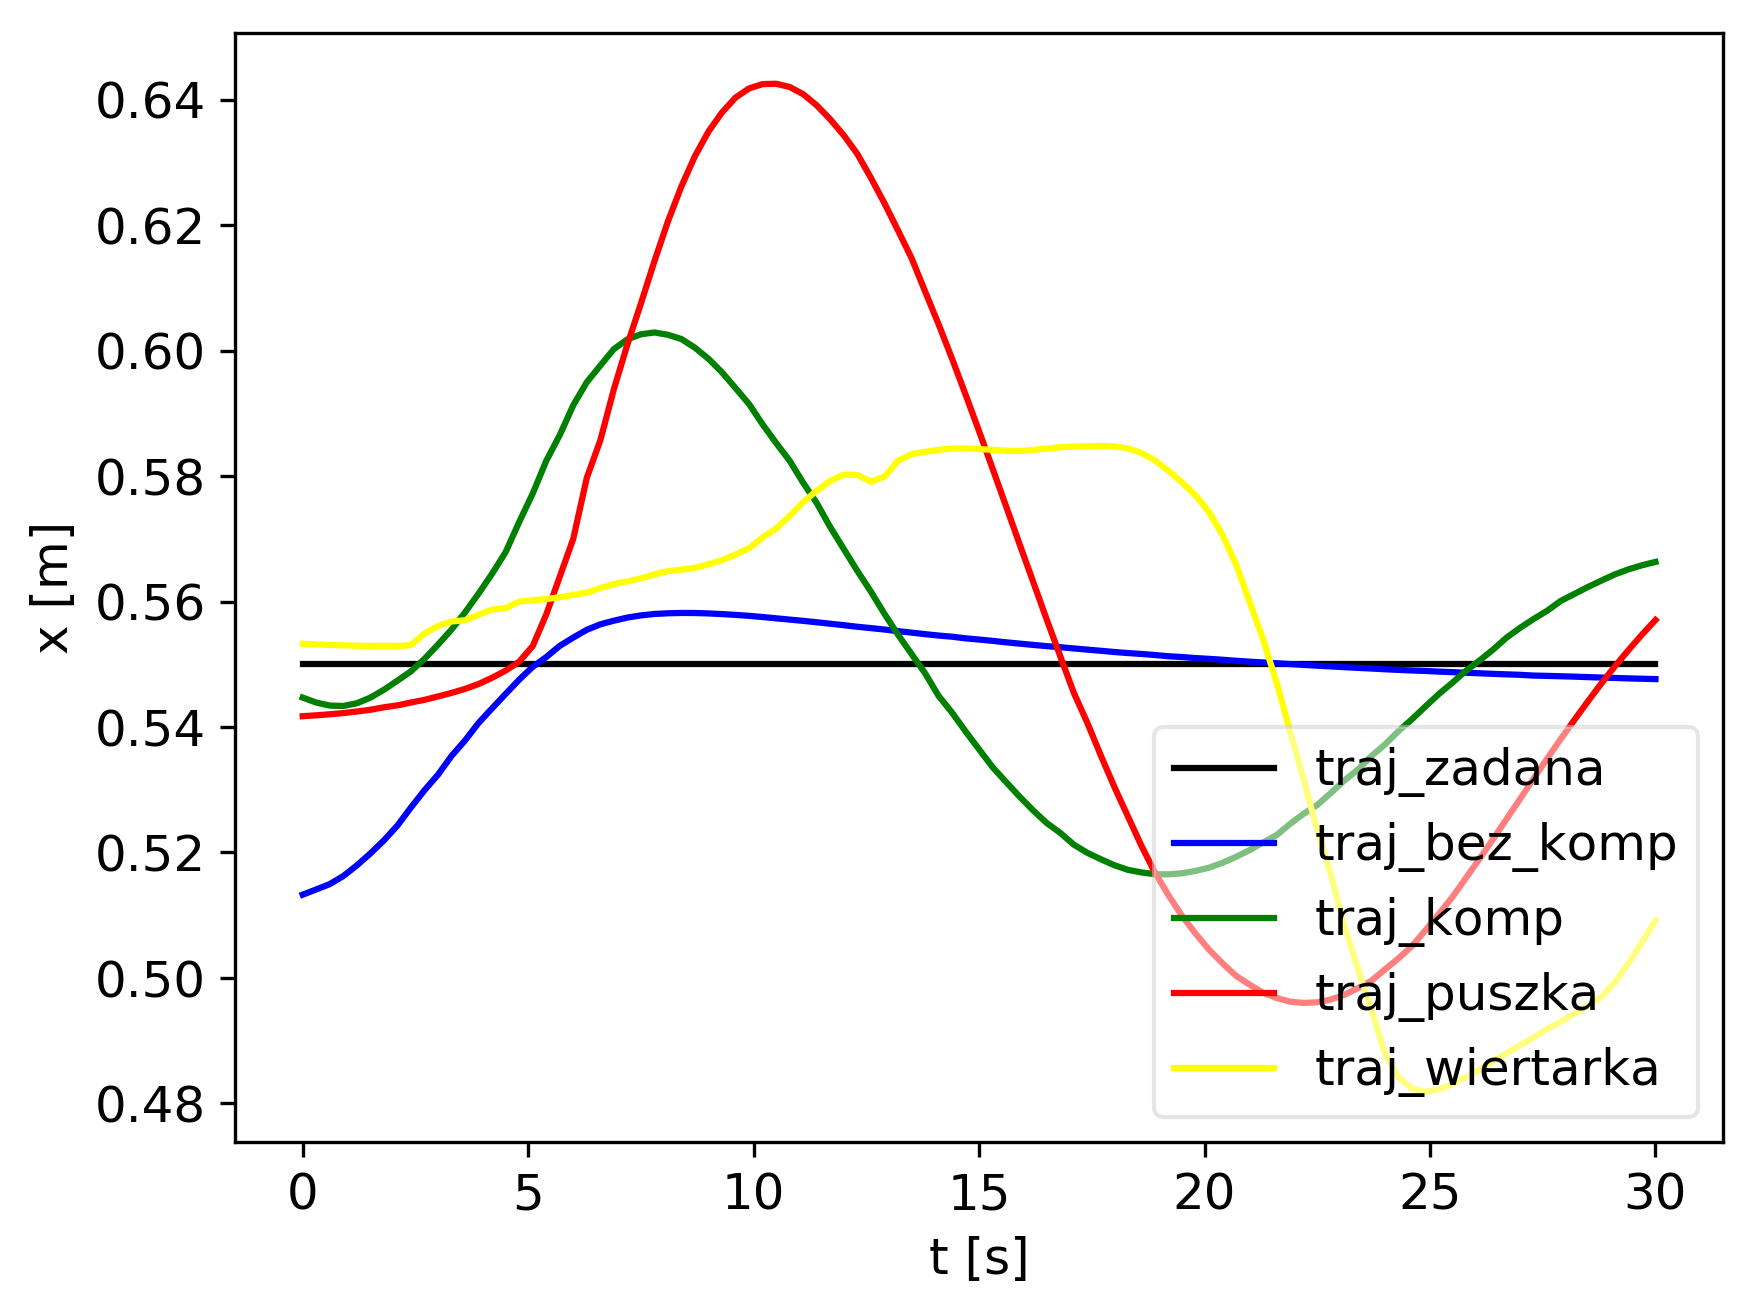
\includegraphics[width=.45\textwidth]{../../velma/przerobione_testy/out/podn/common_ax.png}
	}
	\hfill
	\subfigure[Oś $Y$]{
		\label{fig:podn_ay}
		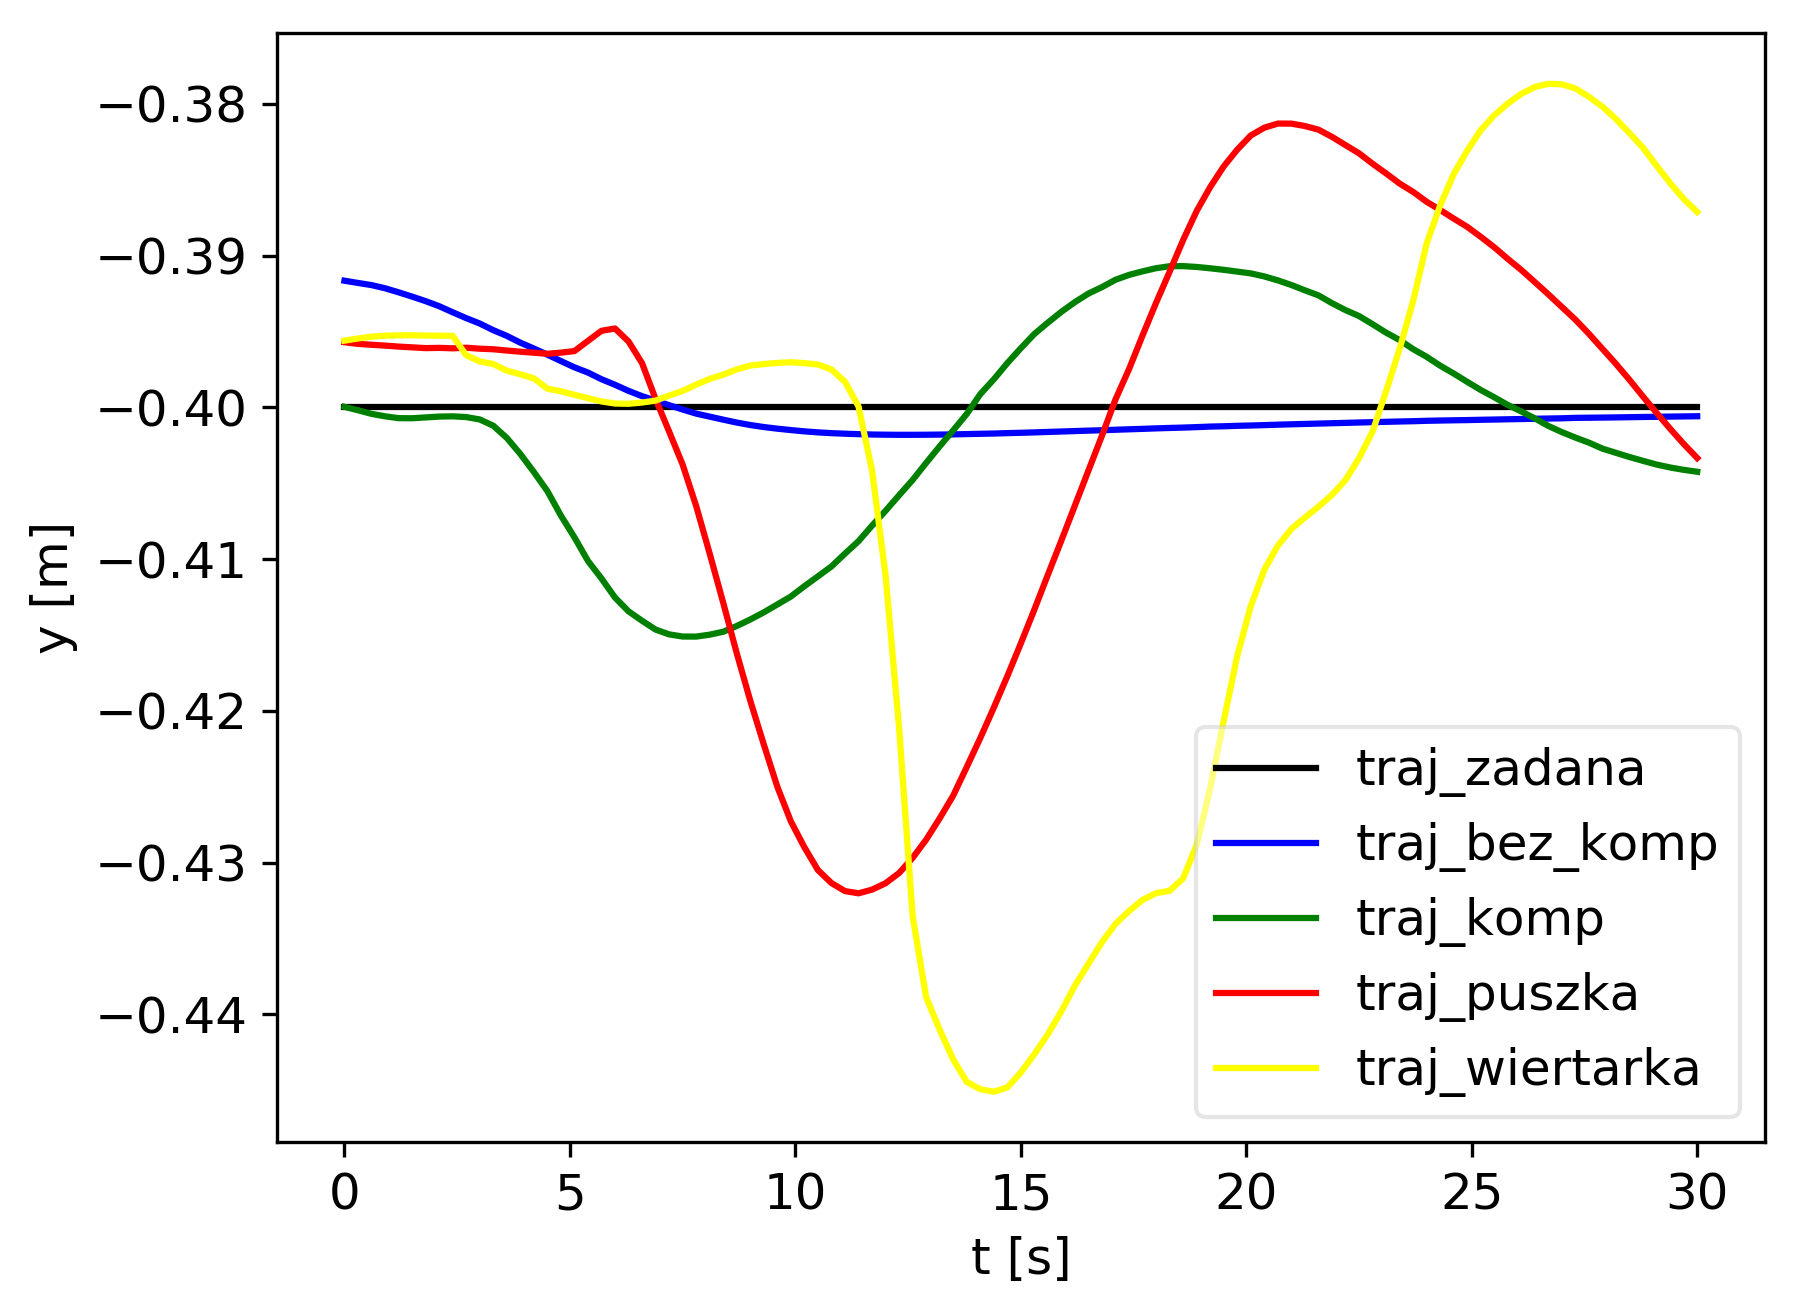
\includegraphics[width=.45\textwidth]{../../velma/przerobione_testy/out/podn/common_ay.png}
	}
	
	\subfigure[Oś $Z$]{
		\label{fig:podn_az}
		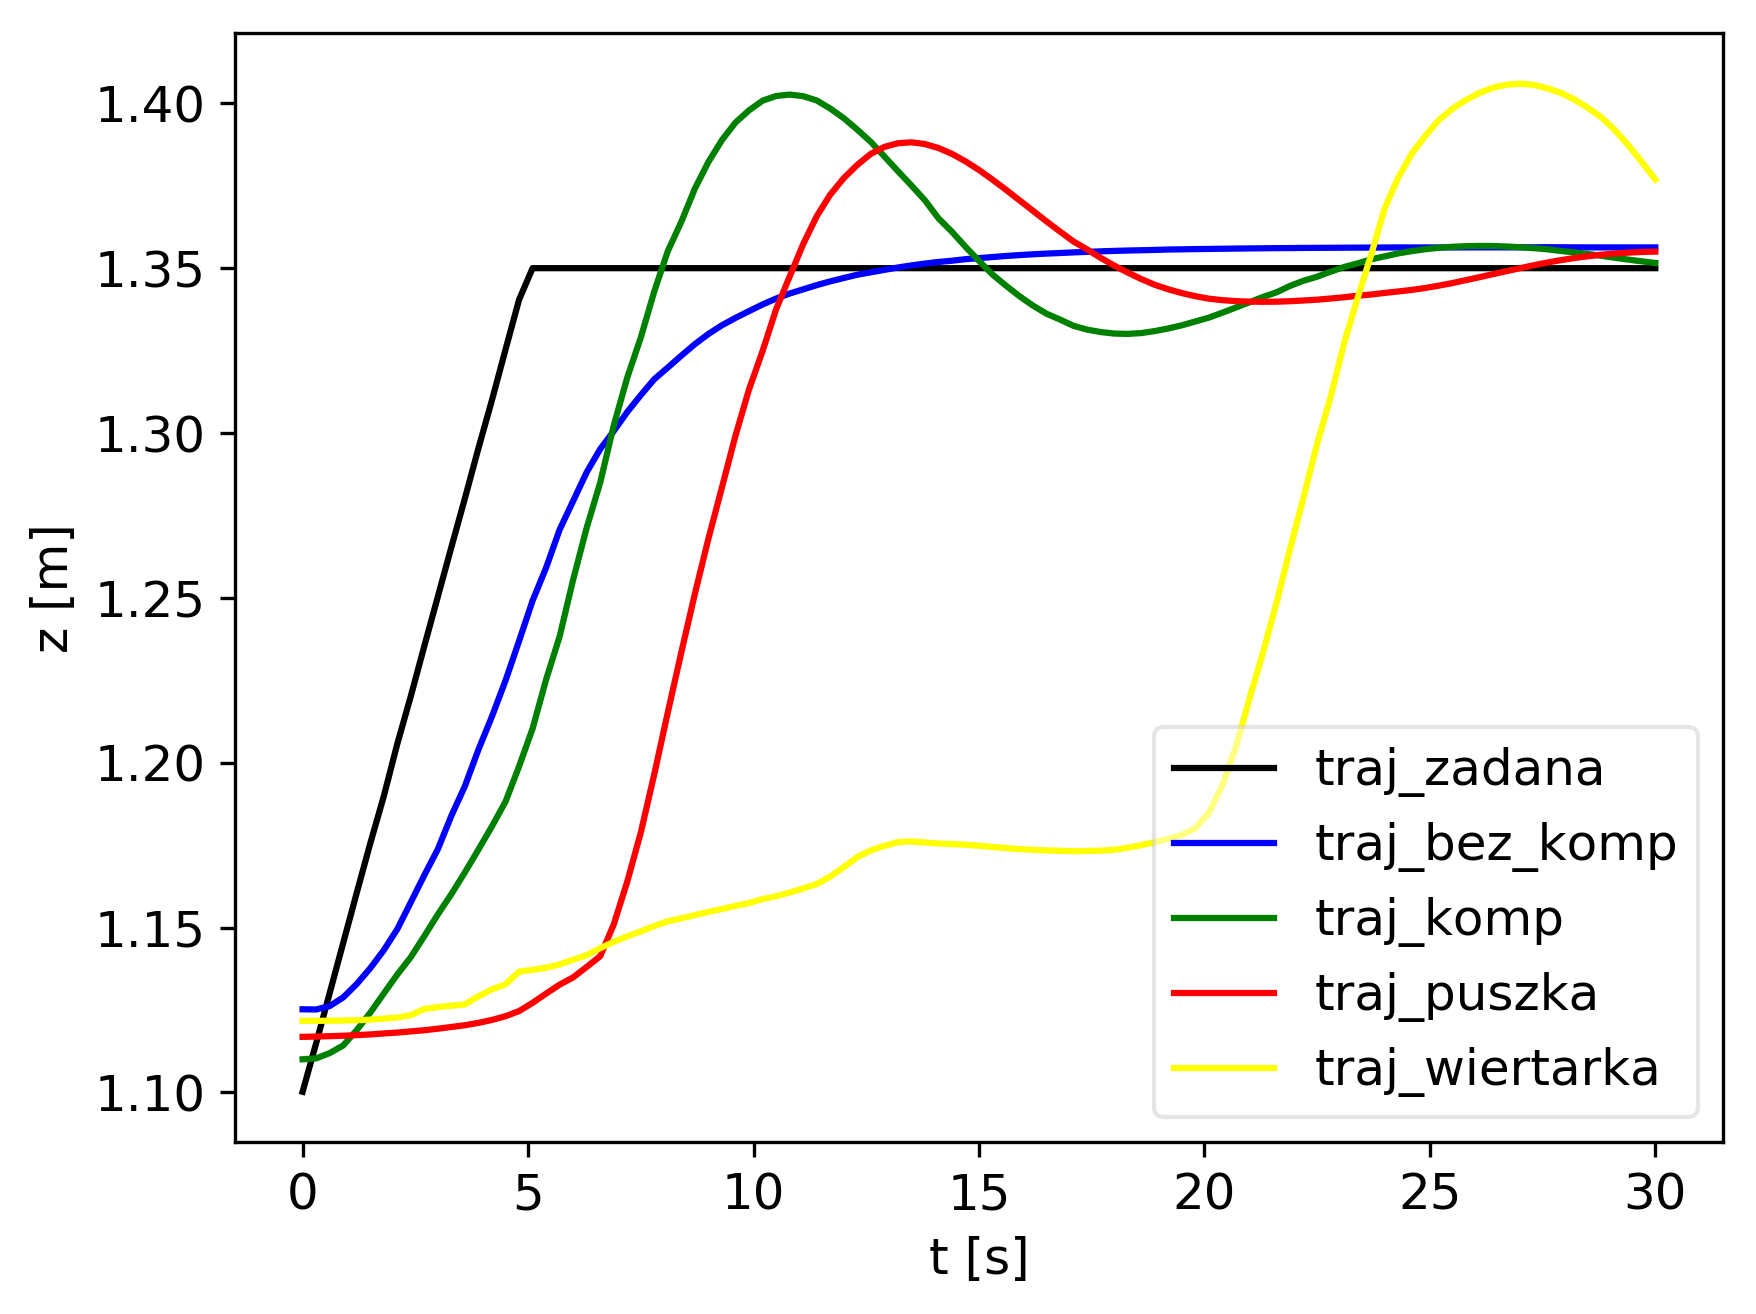
\includegraphics[width=.45\textwidth]{../../velma/przerobione_testy/out/podn/common_az.png}
	}

	\caption{Podnoszenie przedmiotu. Porównanie trajektorii pozycji w~zależności od czasu.}
	\label{fig:podn_a}

\end{figure}

\begin{figure}[H]
	\centering
	\subfigure[Brak algorytmu kompensacji]{
		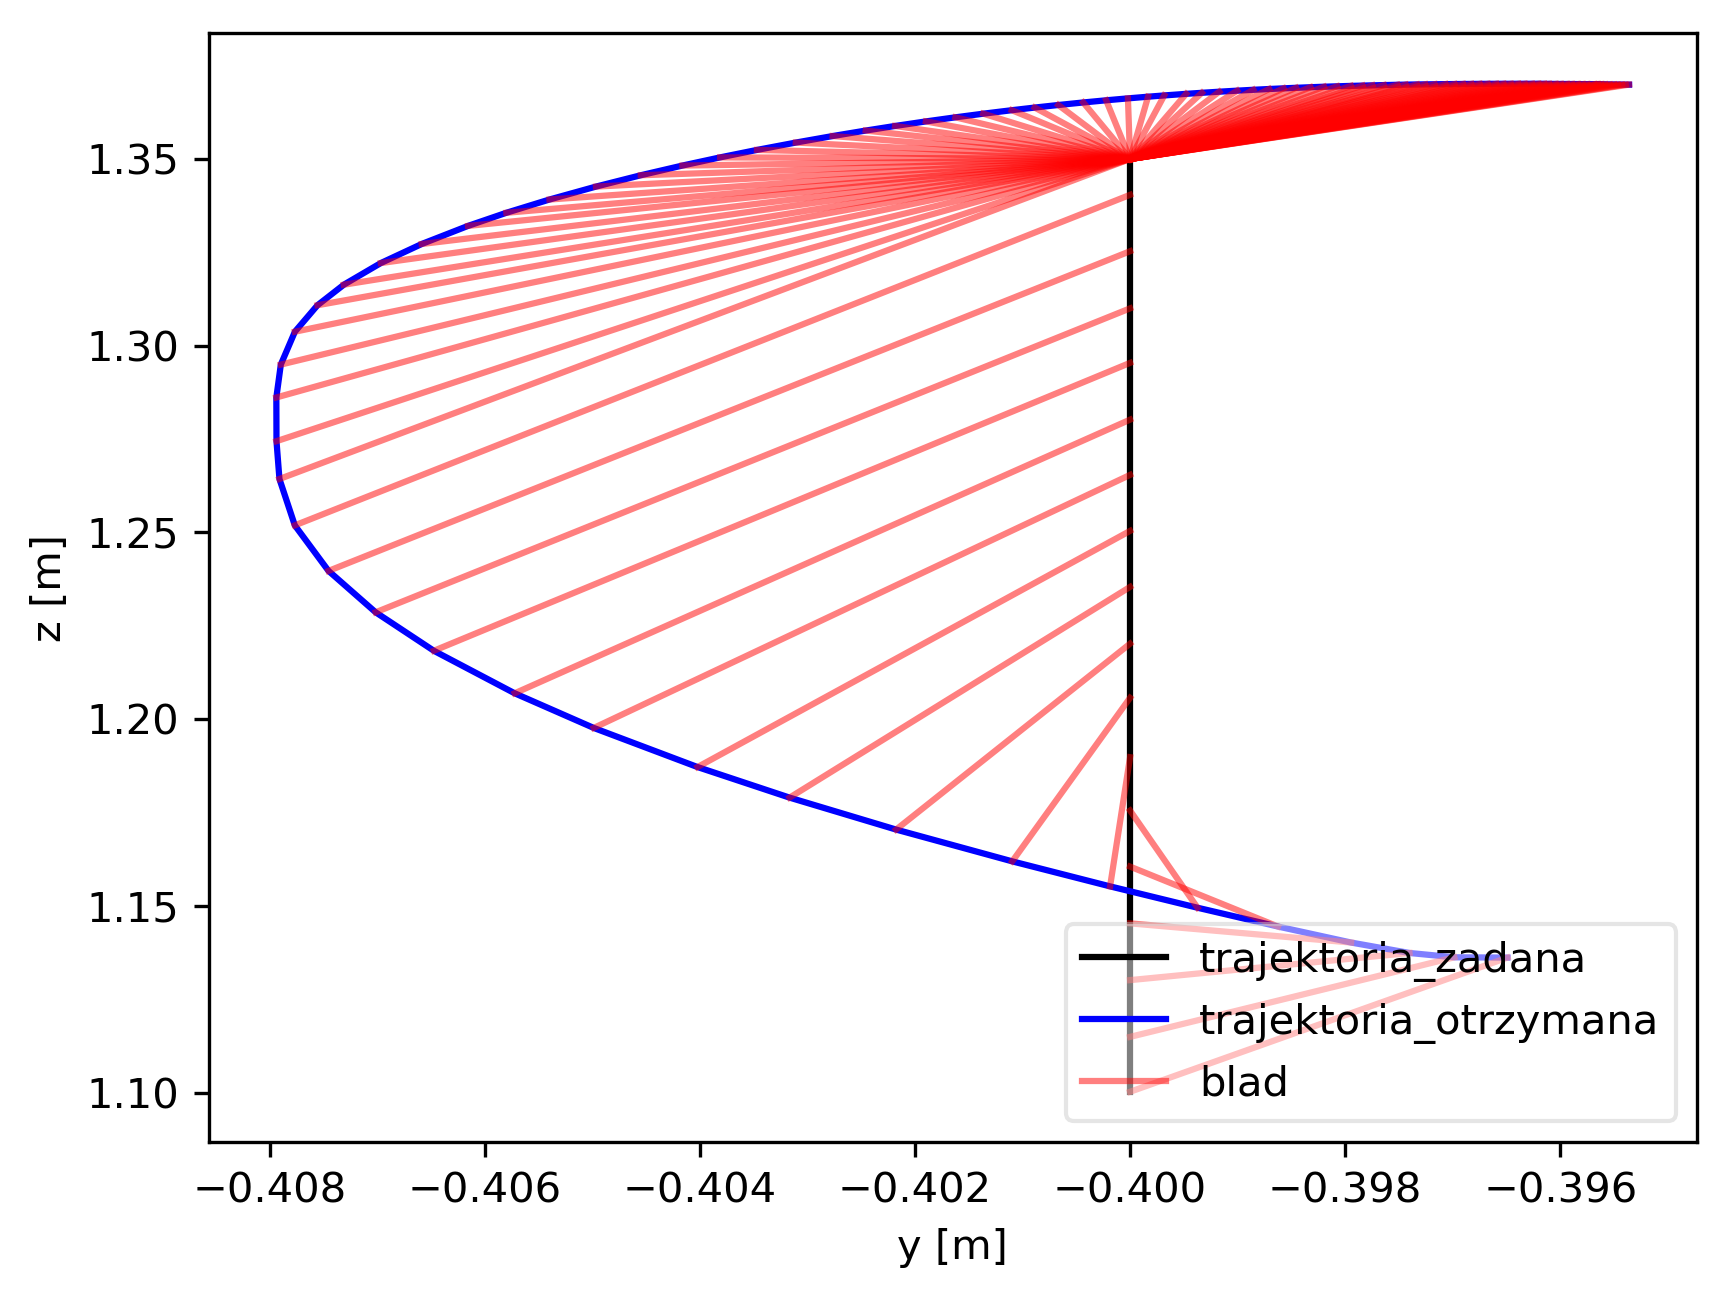
\includegraphics[width=.45\textwidth]{../../velma/przerobione_testy/out/podn/yz_ate_plot_podnoszenie_miekki_bez_brak.png}
	}
	\hfill
	\subfigure[Zalaczony algorytm kompnesacji]{
		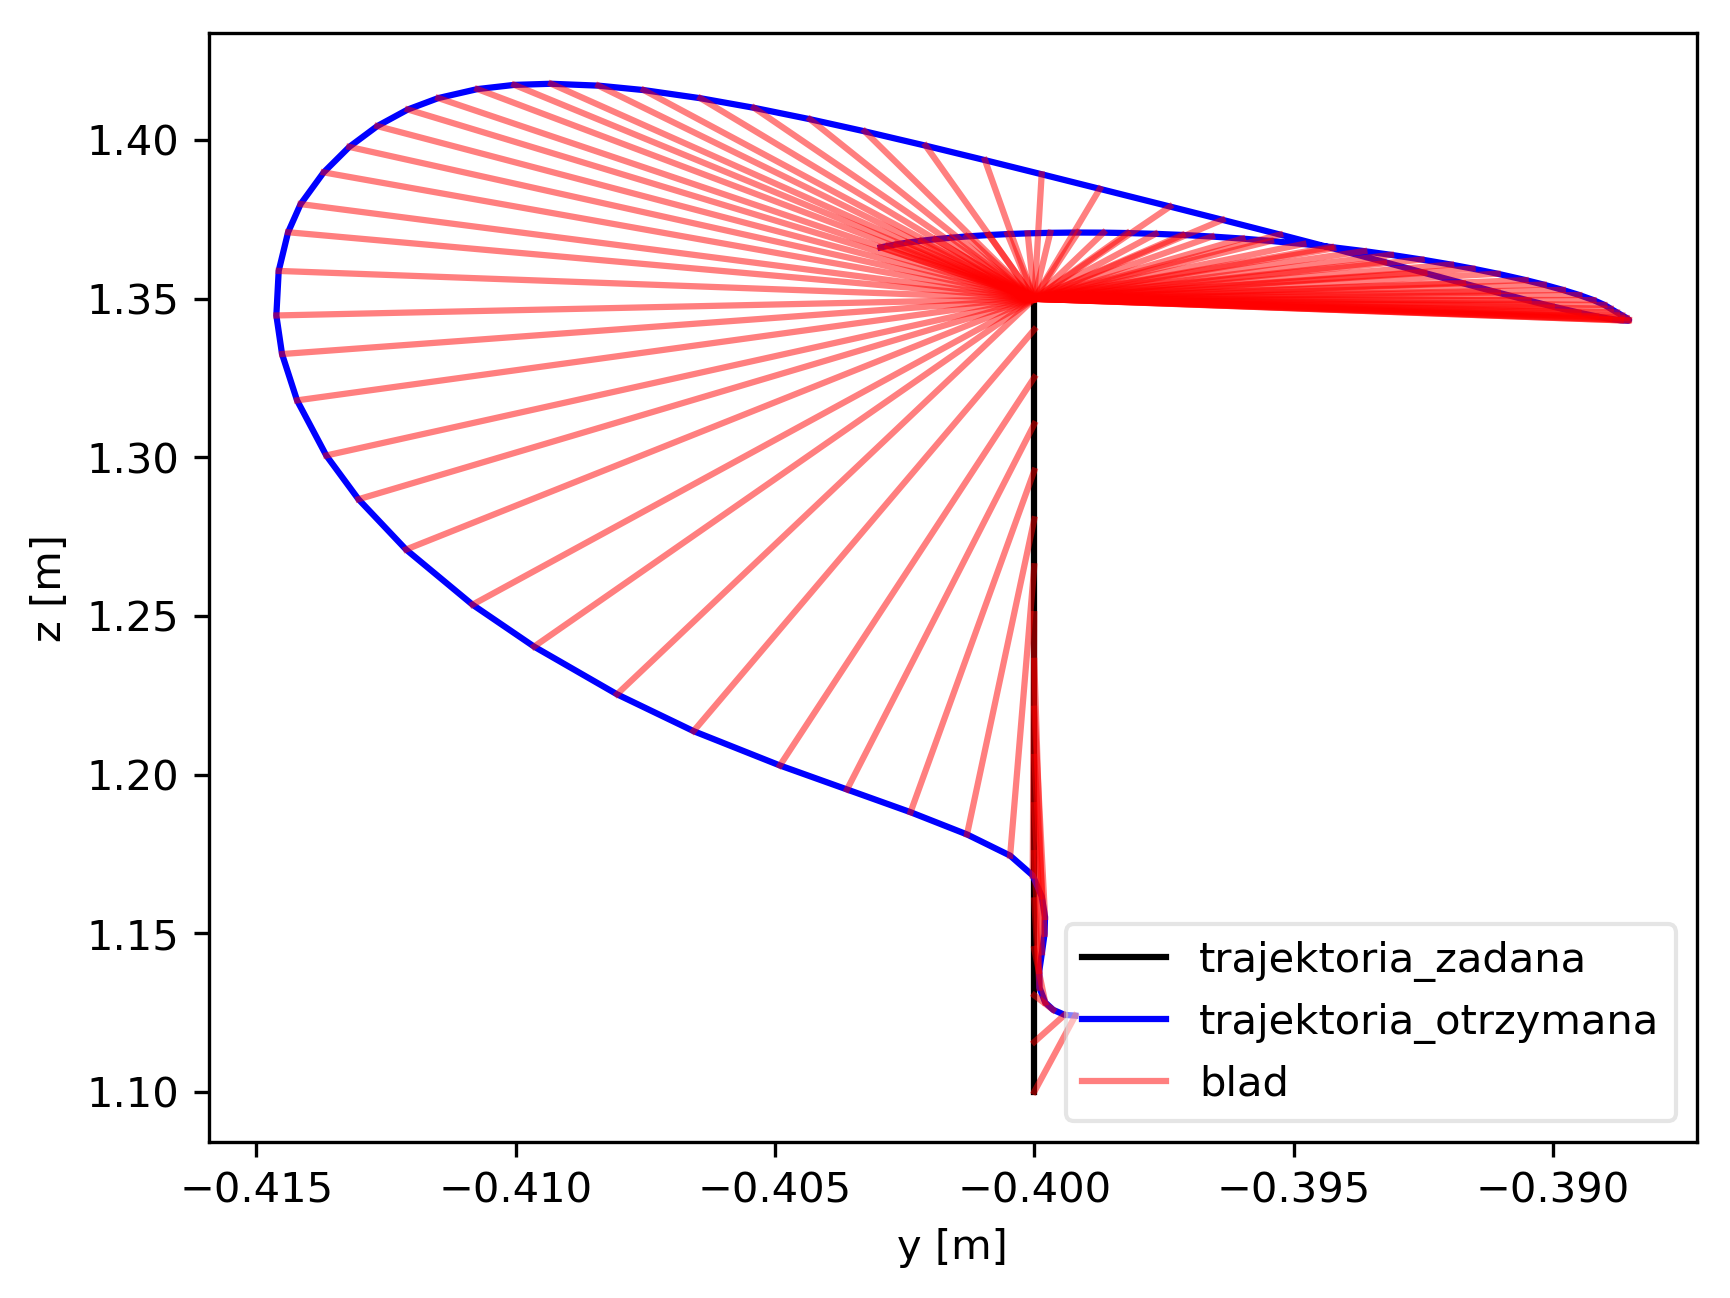
\includegraphics[width=.45\textwidth]{../../velma/przerobione_testy/out/podn/yz_ate_plot_podnoszenie_miekki_komp_brak.png}
	}
	\caption{Podnoszenie przedmiotu. Porównanie trajektorii chwytaka w~osiach $Y$ i~$Z$}
	\label{fig:podn_porow_komp}
\end{figure}

\begin{figure}[H]
	\centering
	\subfigure[Kąt osi $X$]{
		\label{fig:podn_rotx}
		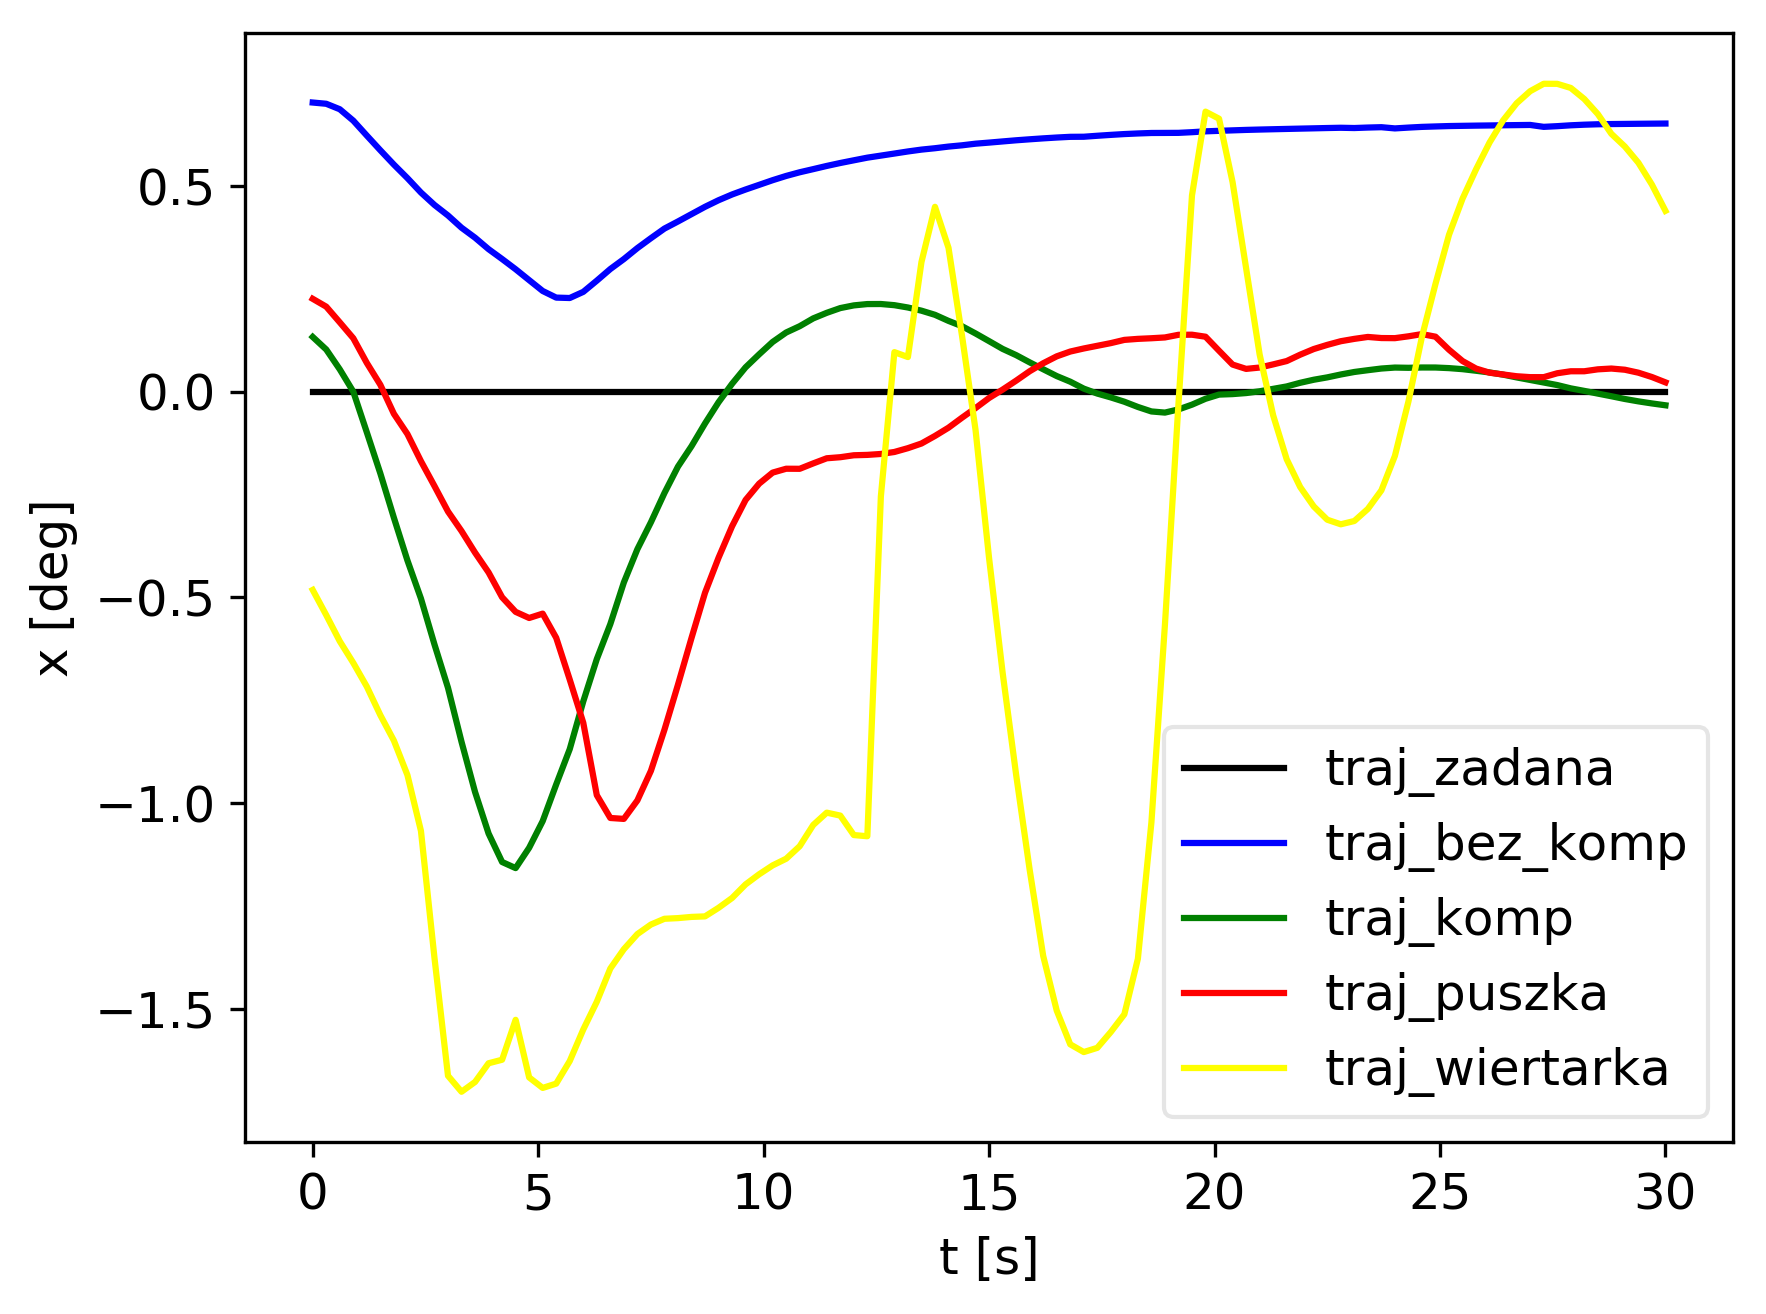
\includegraphics[width=.45\textwidth]{../../velma/przerobione_testy/out/podn/common_rotx.png}
	}
	\hfill
	\subfigure[Kąt osi $Y$]{
		\label{fig:do_gory_roty}
		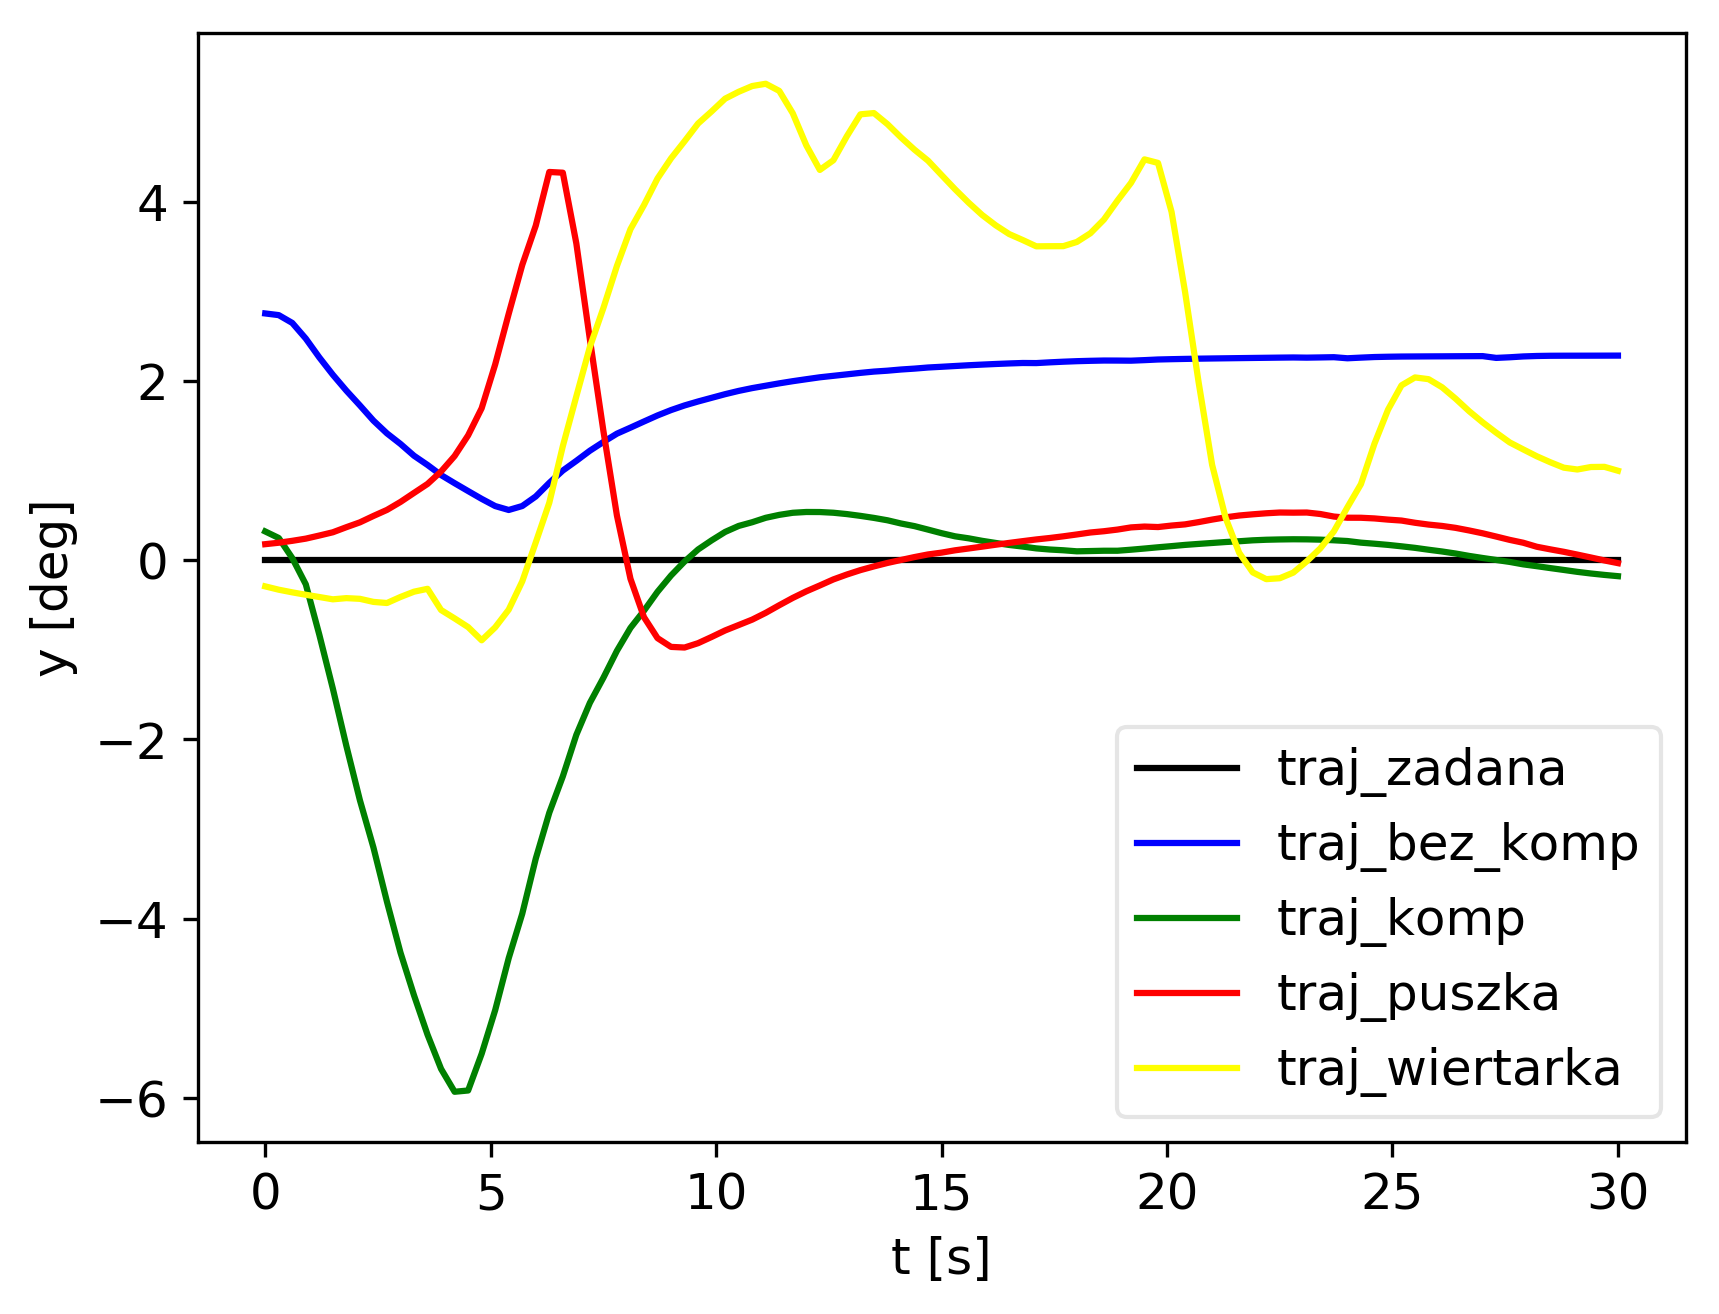
\includegraphics[width=.45\textwidth]{../../velma/przerobione_testy/out/podn/common_roty.png}
	}
	

	\subfigure[Kąt osi $Z$]{
		\label{fig:podn_rotz}
		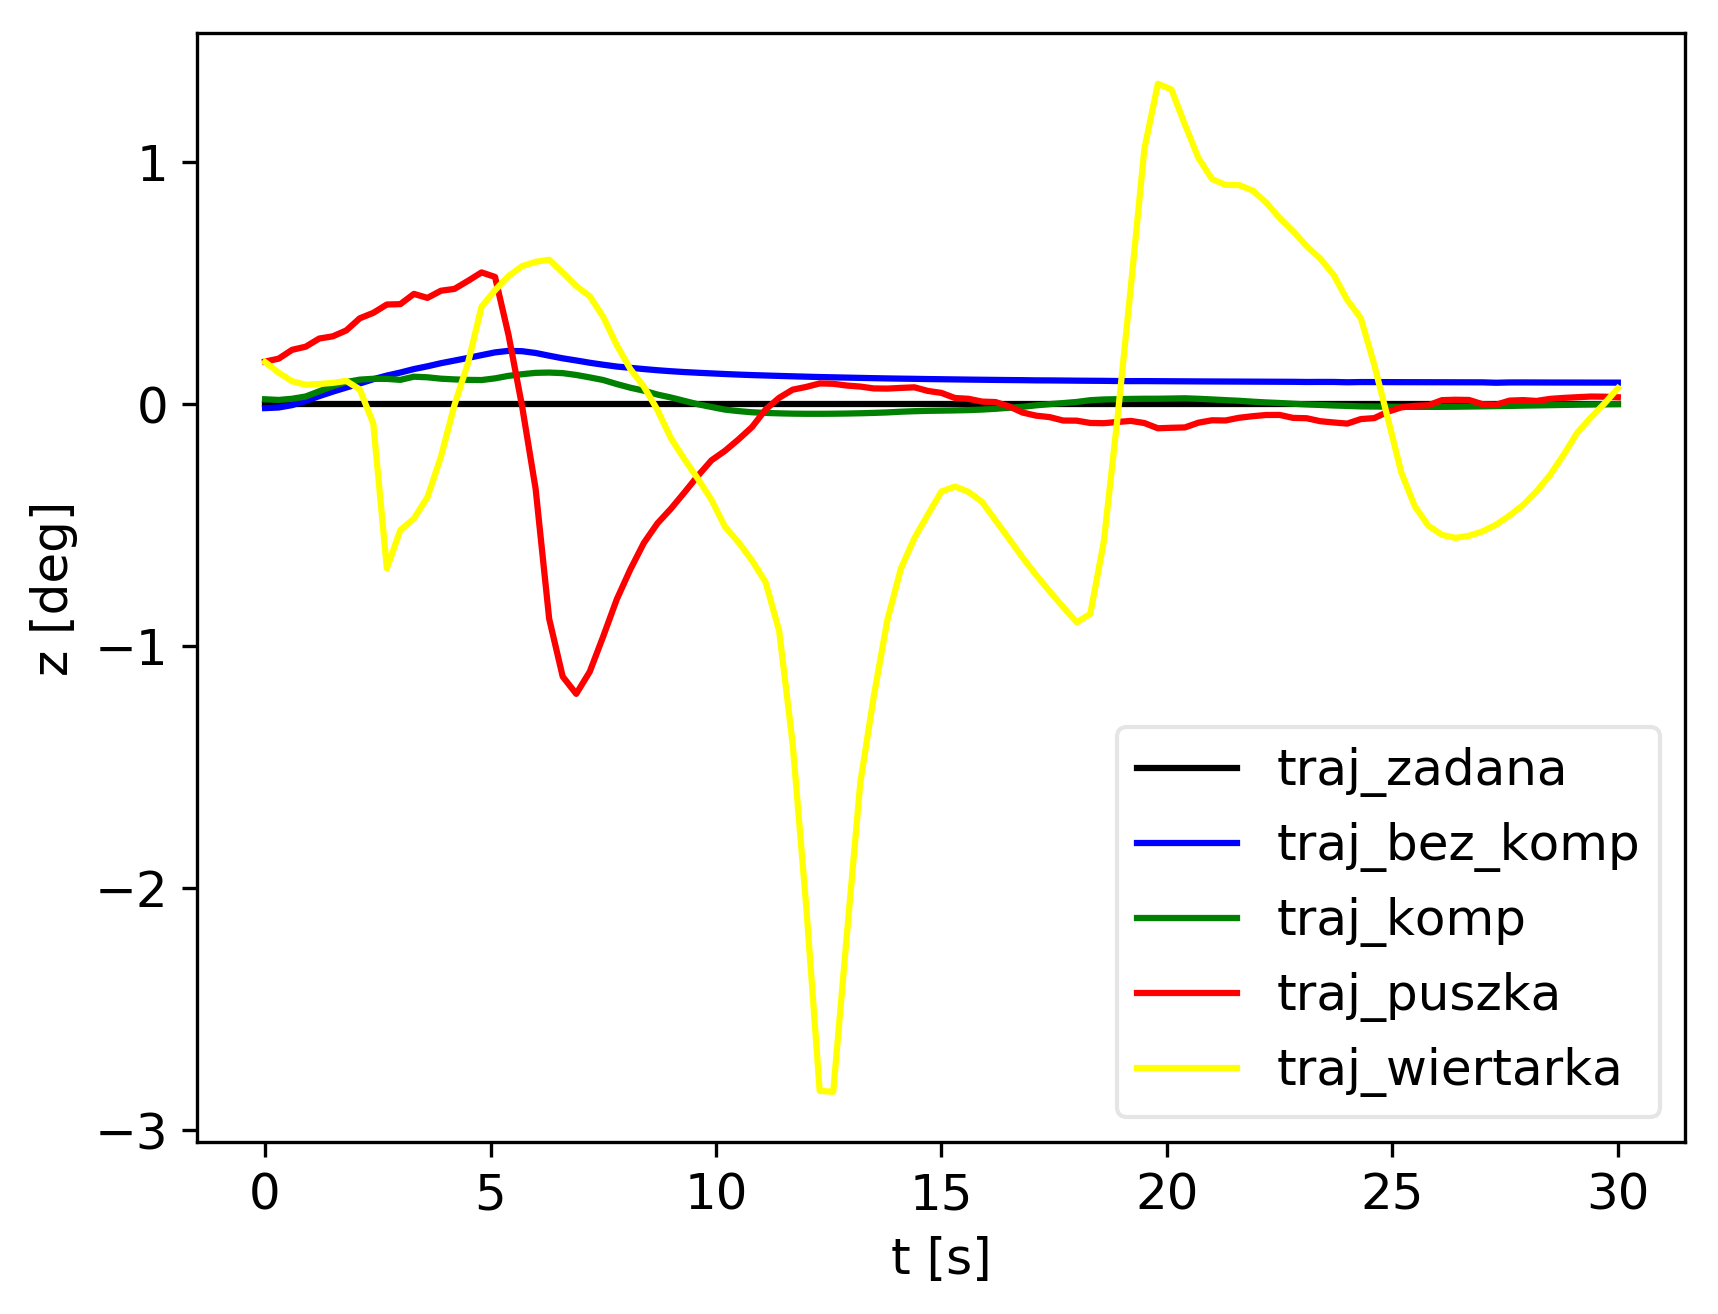
\includegraphics[width=.45\textwidth]{../../velma/przerobione_testy/out/podn/common_rotz.png}
	}

	\caption{Podnoszenie przedmiotu. Porównanie trajektorii kątów w~notacji Eulera w~zależności od czasu.}
	\label{fig:podn_rot}

\end{figure}



\begin{figure}
	\centering
	\subfigure[Trajektoria z~chwycona puszka]{
		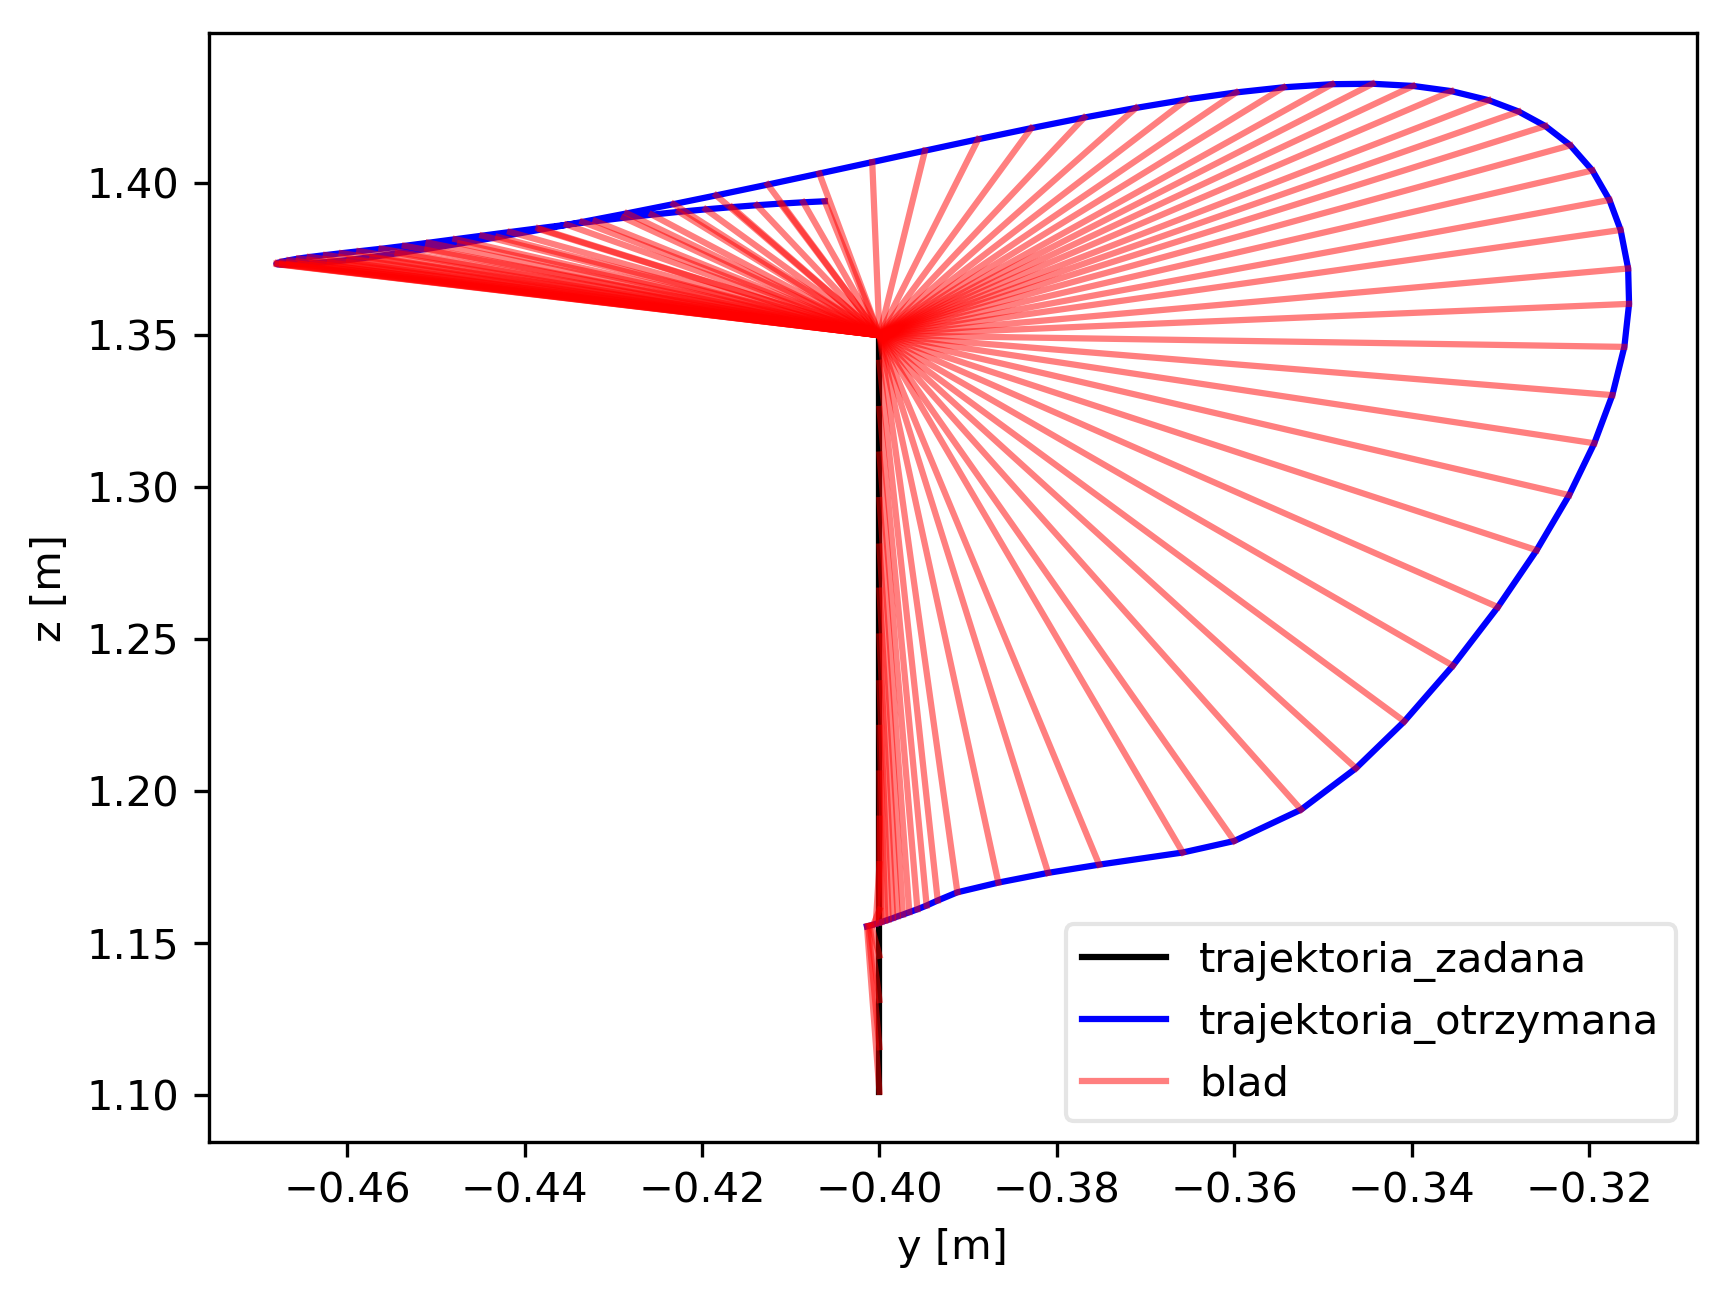
\includegraphics[width=.45\textwidth]{../../velma/przerobione_testy/out/podn/yz_ate_plot_podnoszenie_miekki_komp_piwo.png}
	}
	\hfill
	\subfigure[Trajektoria z~chwycona wiertarka]{
		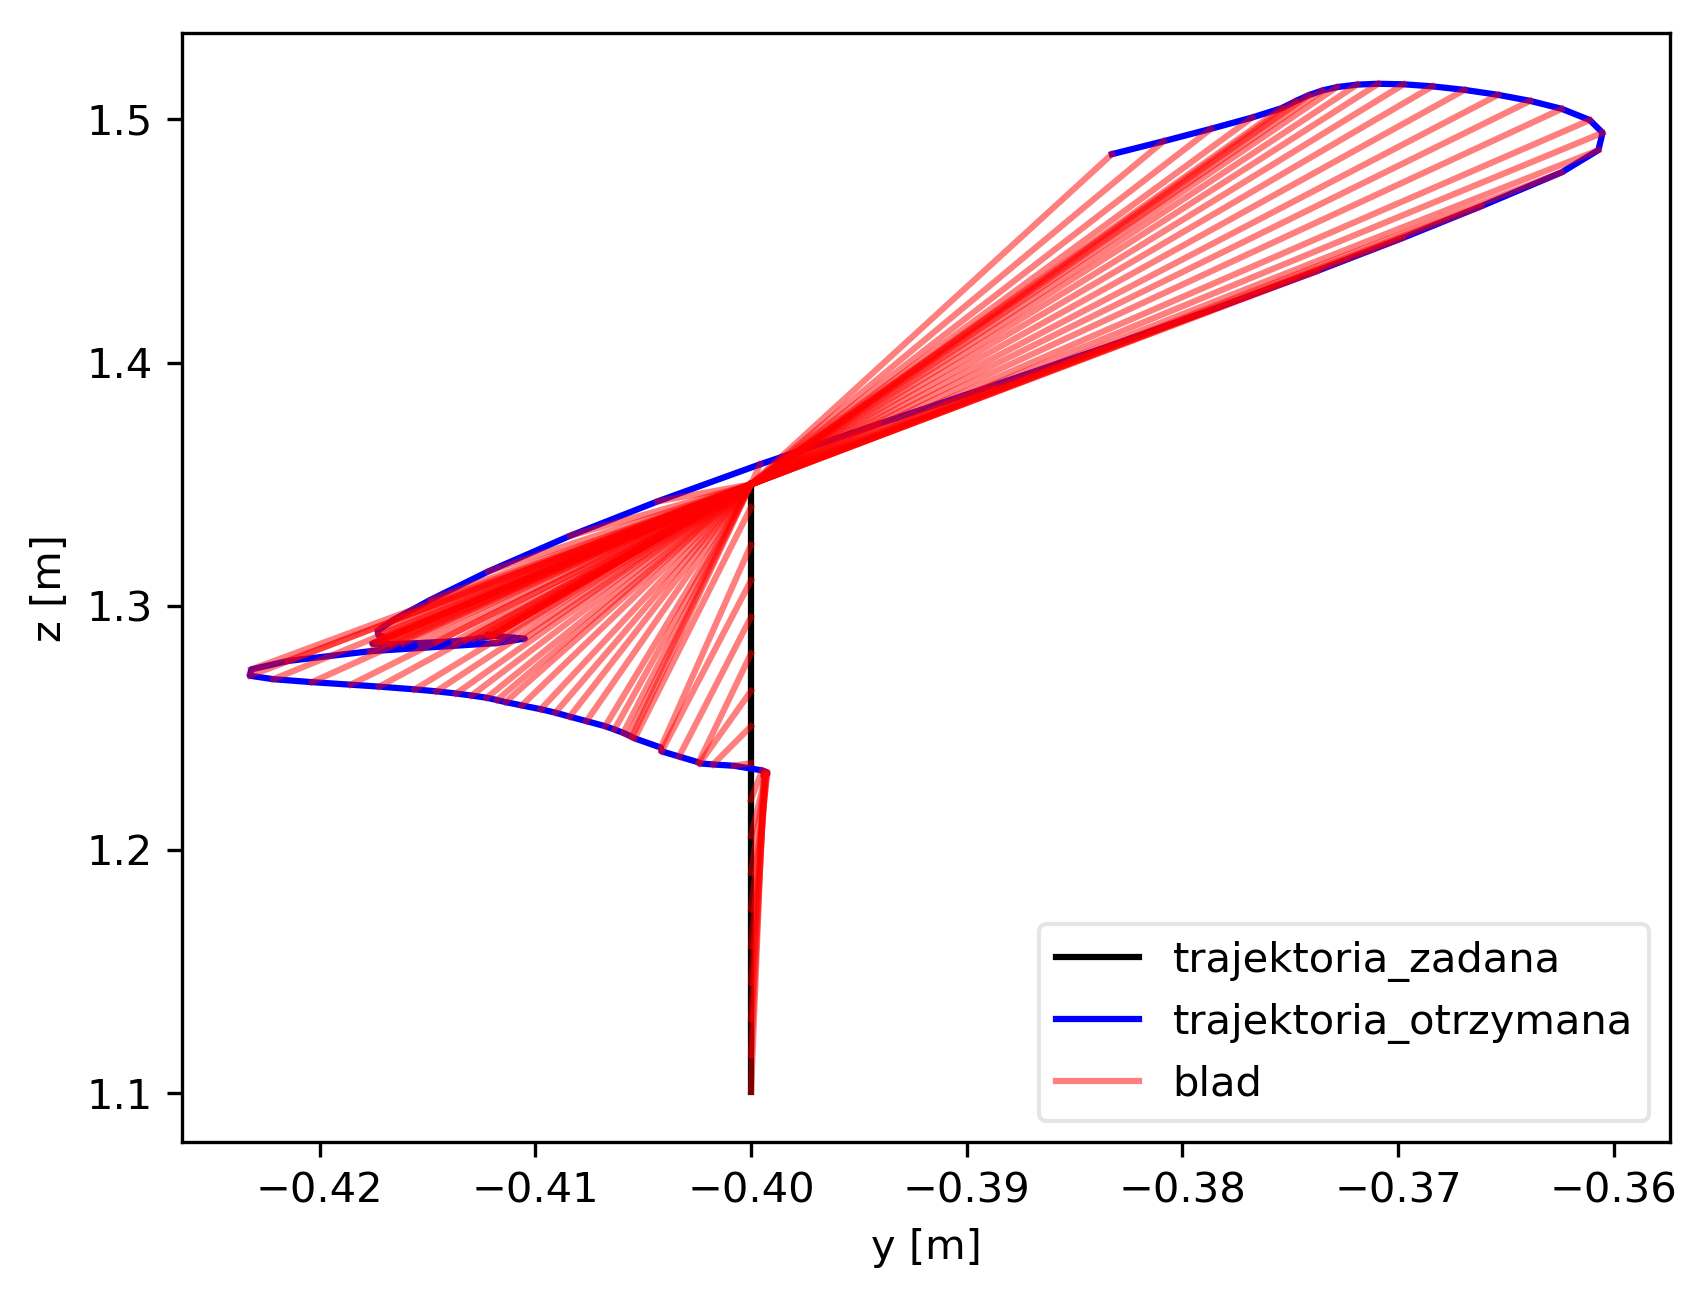
\includegraphics[width=.45\textwidth]{../../velma/przerobione_testy/out/podn/yz_ate_plot_podnoszenie_miekki_komp_wiertarka.png}
	}
	\caption{Podnoszenie przedmiotu. Porównanie trajektorii chwytaka w~osiach $Y$ i~$Z$}
	\label{fig:podn_porow_przedm}
\end{figure}


\begin{figure}[H]
	\centering
	\subfigure[Brak algorytmu kompensacji]{
		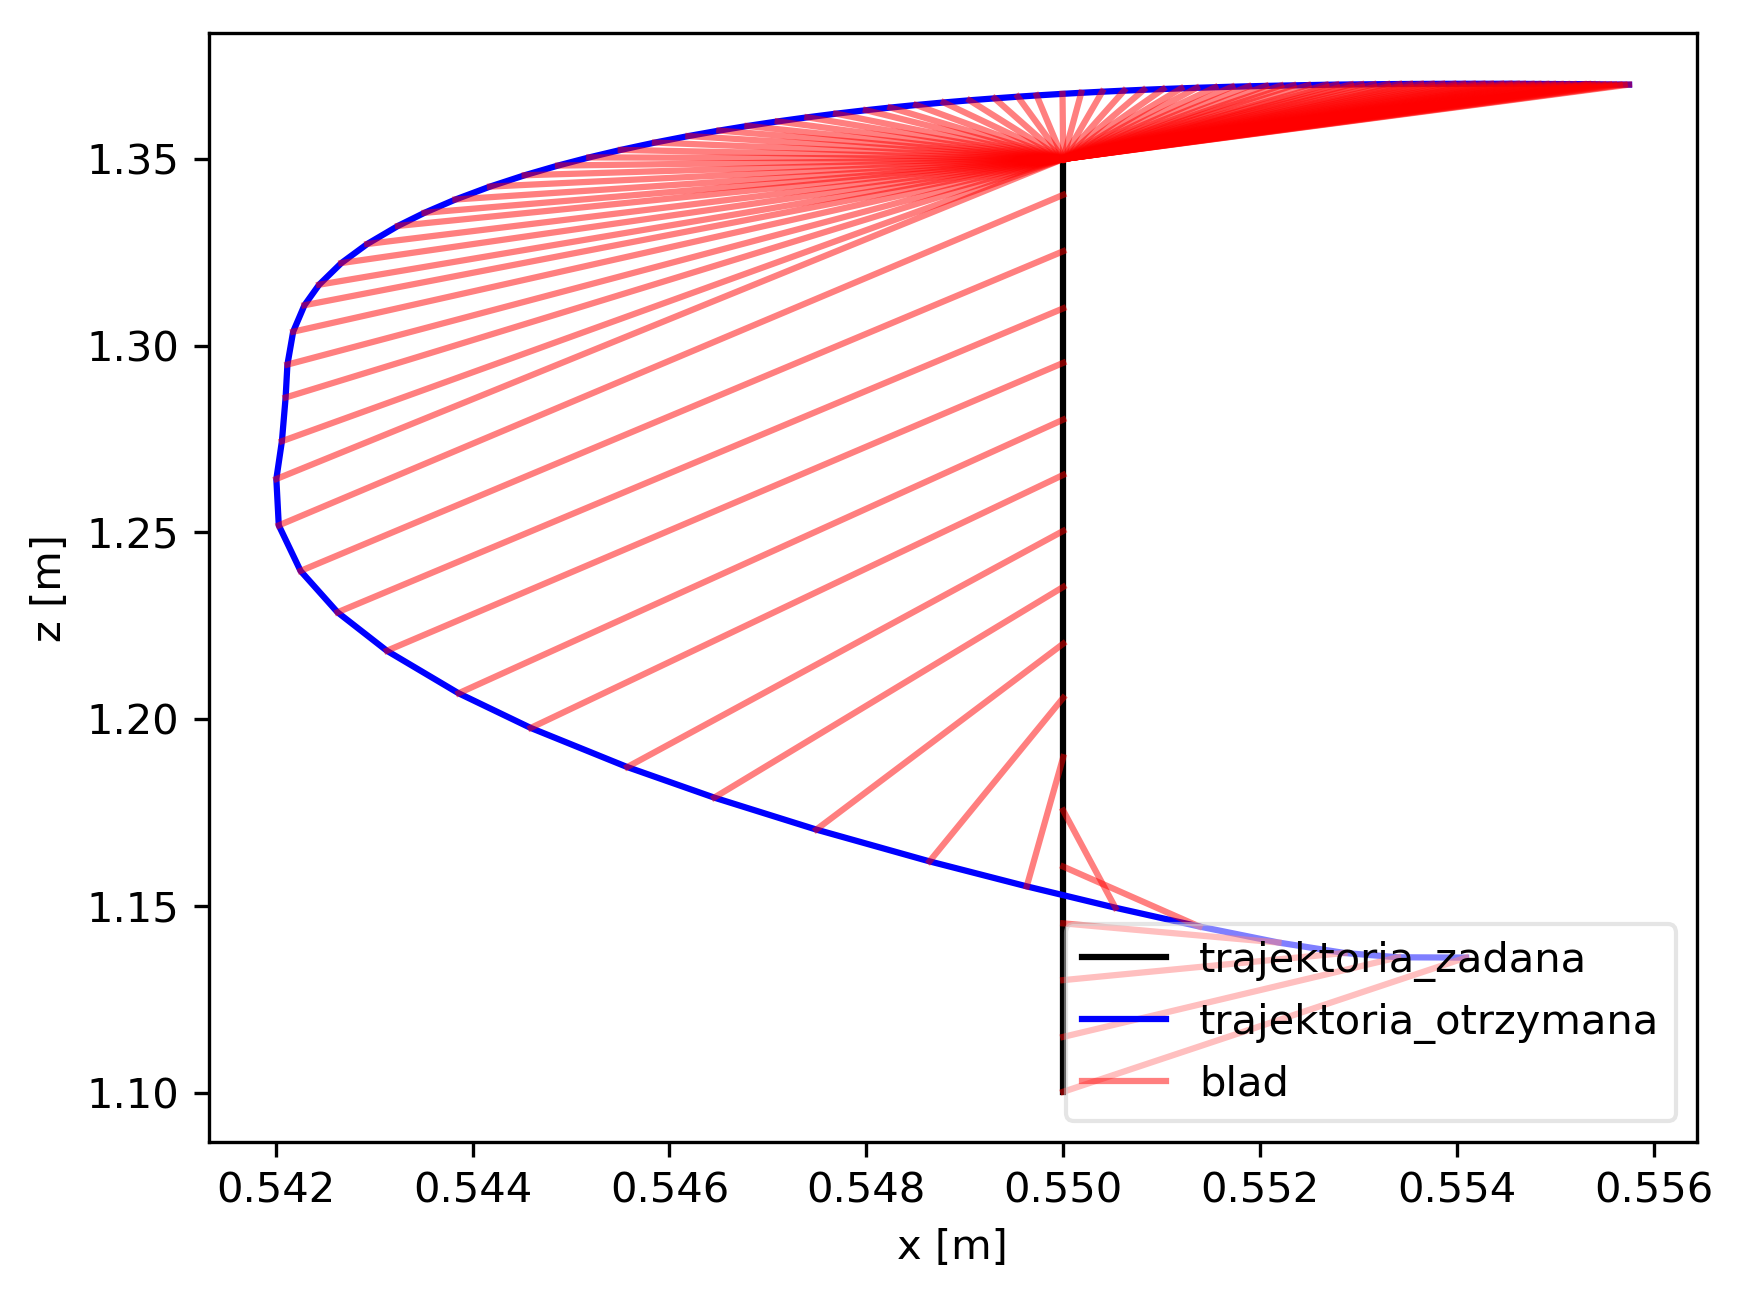
\includegraphics[width=.45\textwidth]{../../velma/przerobione_testy/out/podn/xz_ate_plot_podnoszenie_miekki_bez_brak.png}
	}
	\hfill
	\subfigure[Zalaczony algorytm kompnesacji]{
		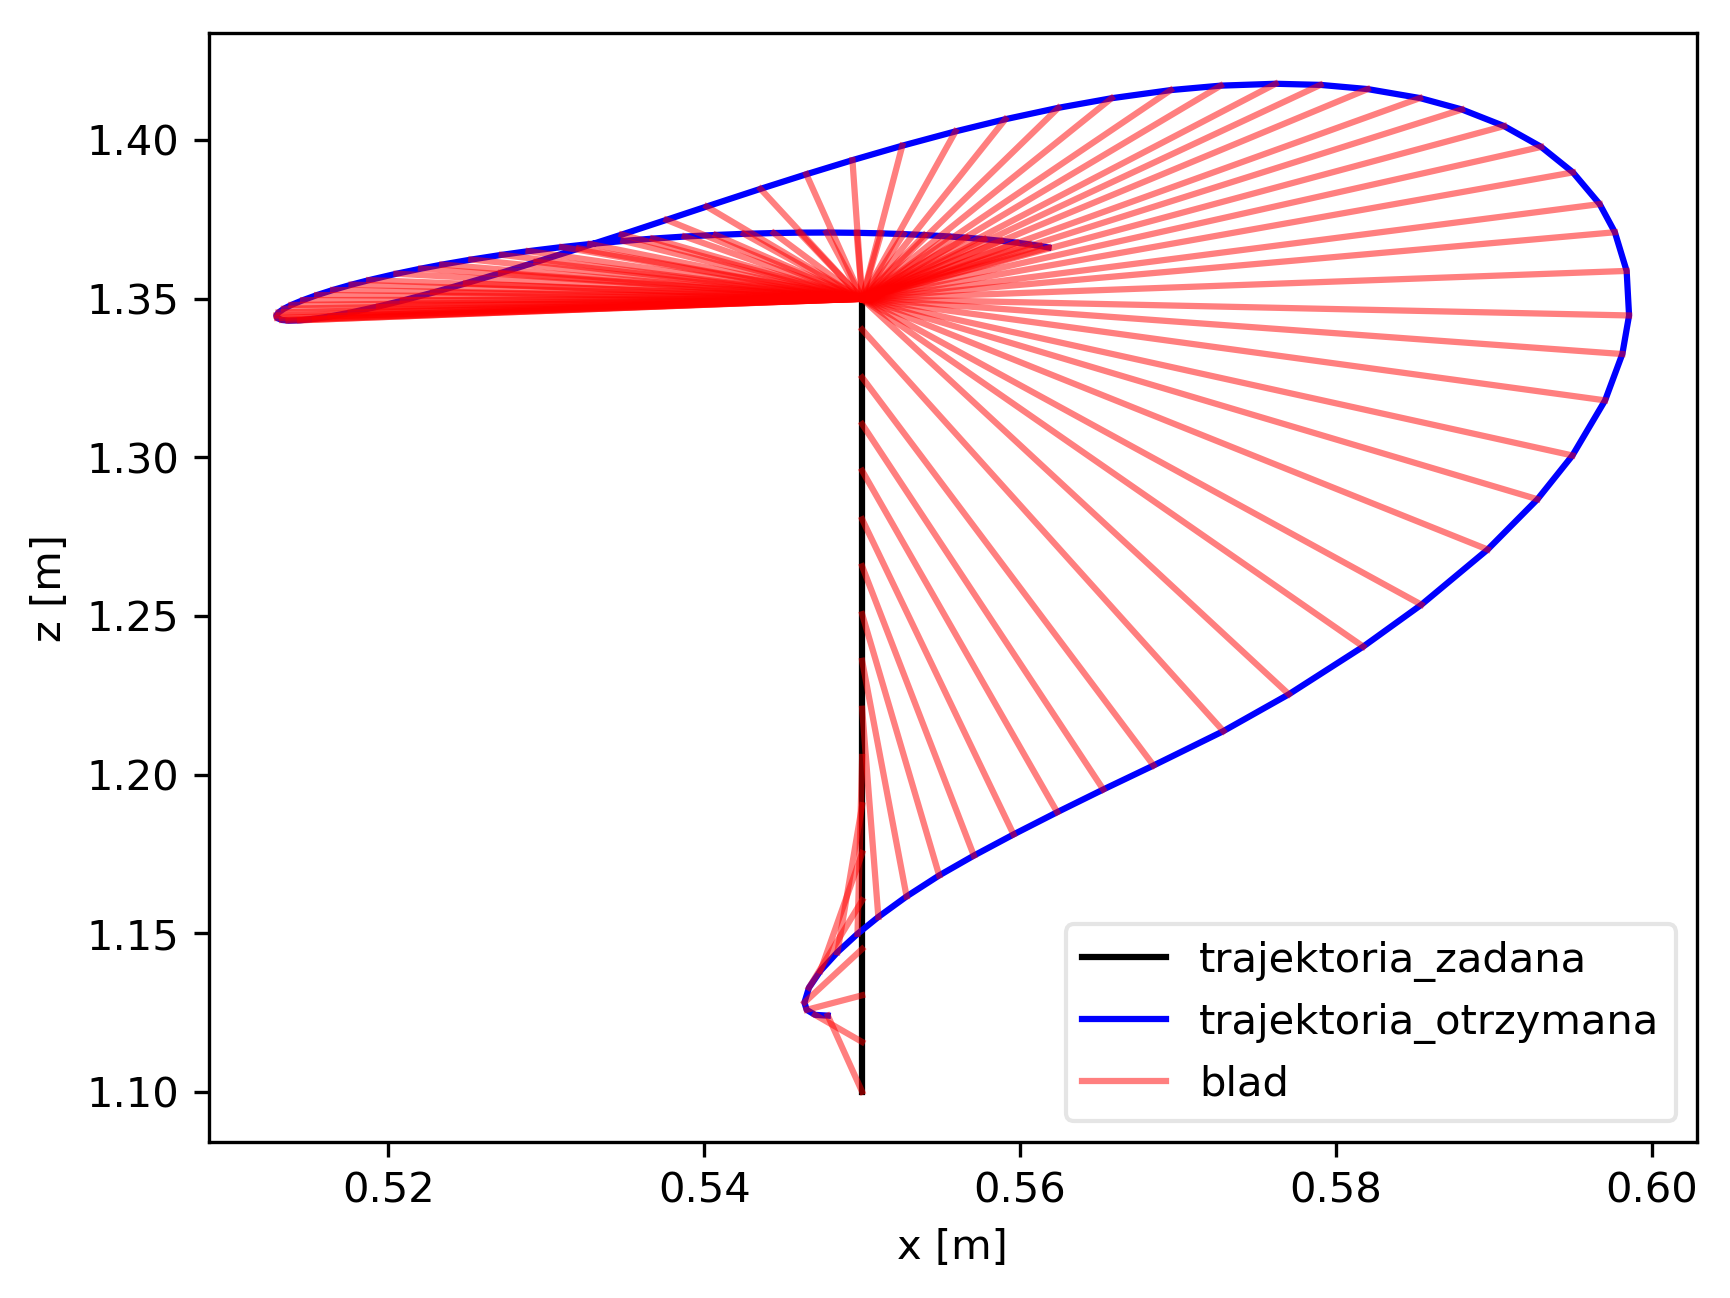
\includegraphics[width=.45\textwidth]{../../velma/przerobione_testy/out/podn/xz_ate_plot_podnoszenie_miekki_komp_brak.png}
	}
	\caption{Podnoszenie przedmiotu. Porównanie trajektorii chwytaka w~osiach $X$ i~$Z$}
	\label{fig:podn_porow_komp_bok}
\end{figure}

\begin{figure}[H]
	\centering
	\subfigure[Trajektoria z~chwycona puszka]{
		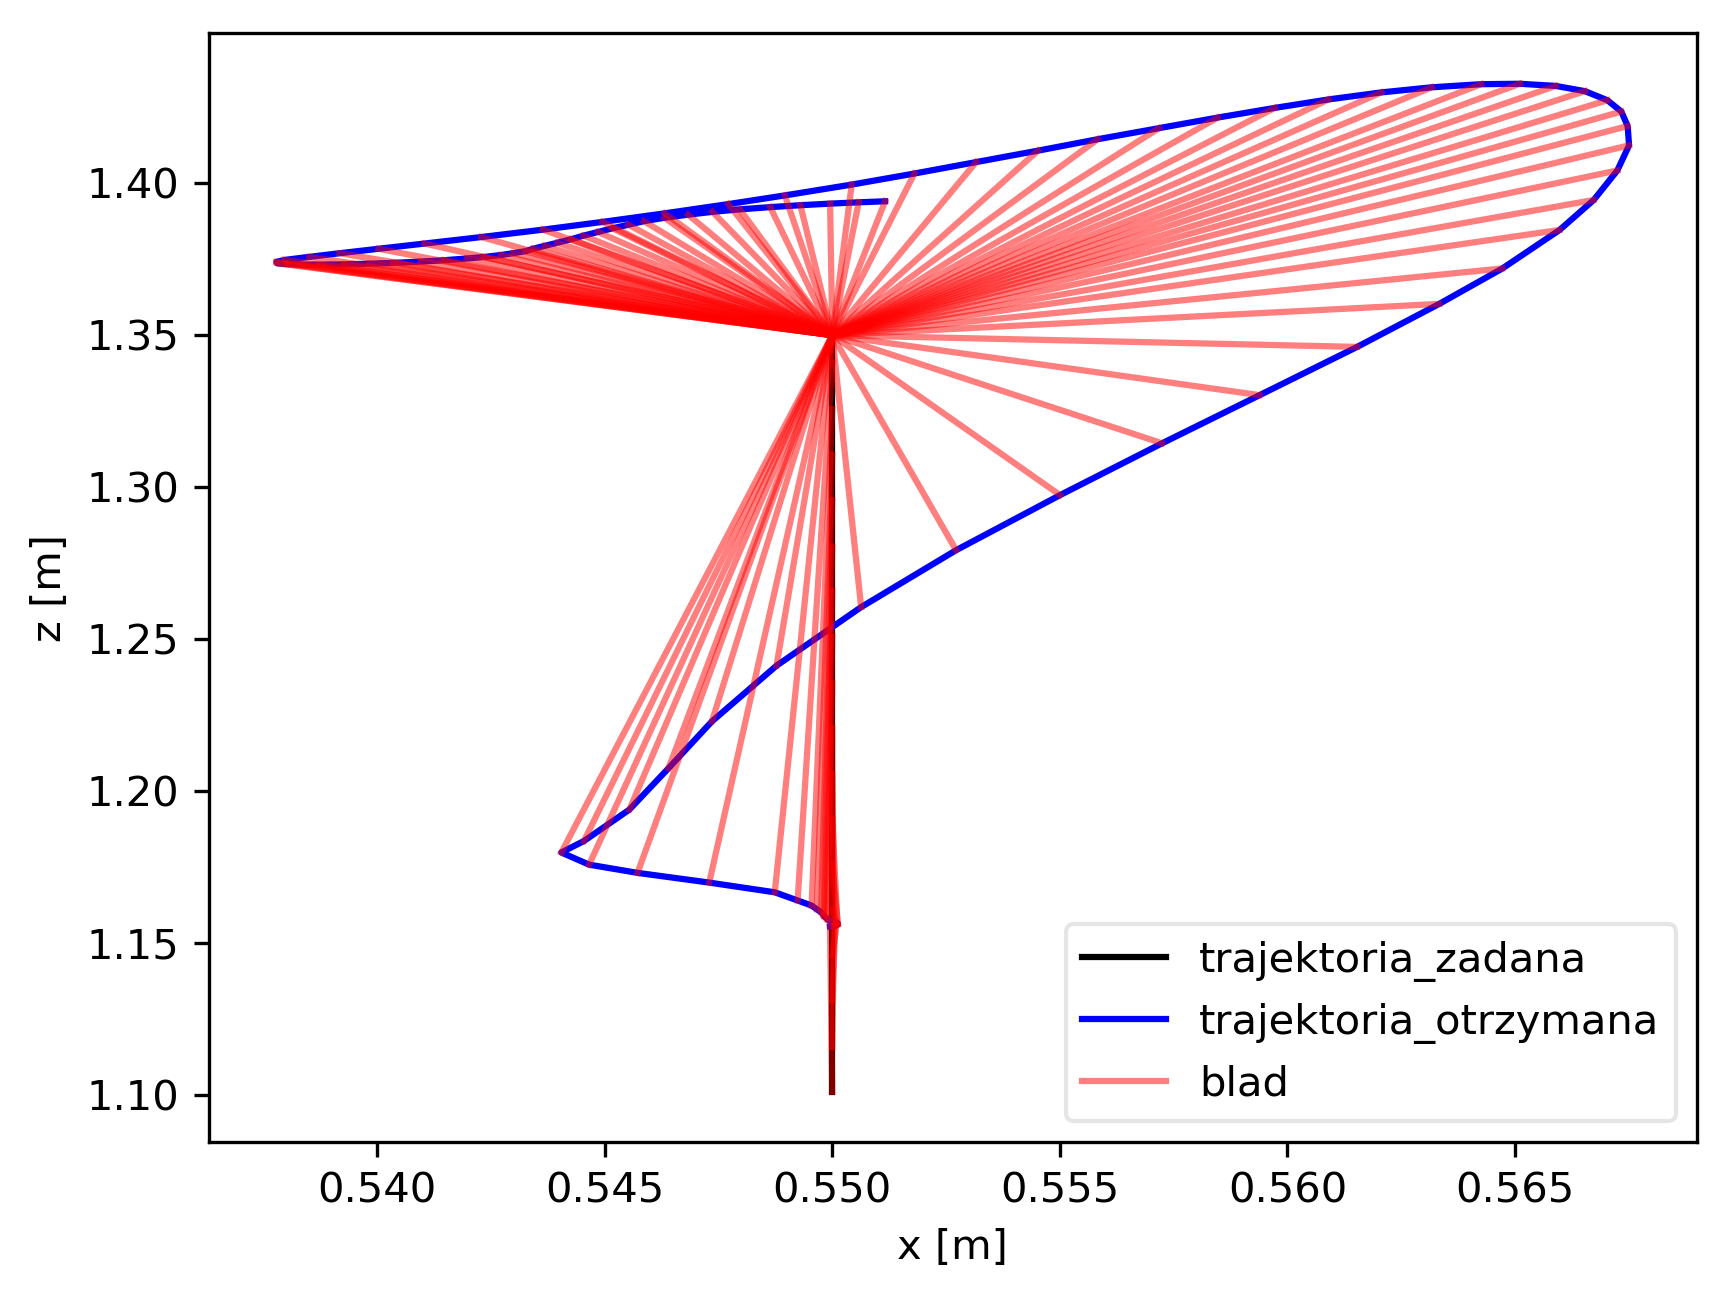
\includegraphics[width=.45\textwidth]{../../velma/przerobione_testy/out/podn/xz_ate_plot_podnoszenie_miekki_komp_piwo.png}
	}
	\hfill
	\subfigure[Trajektoria z~chwycona wiertarka]{
		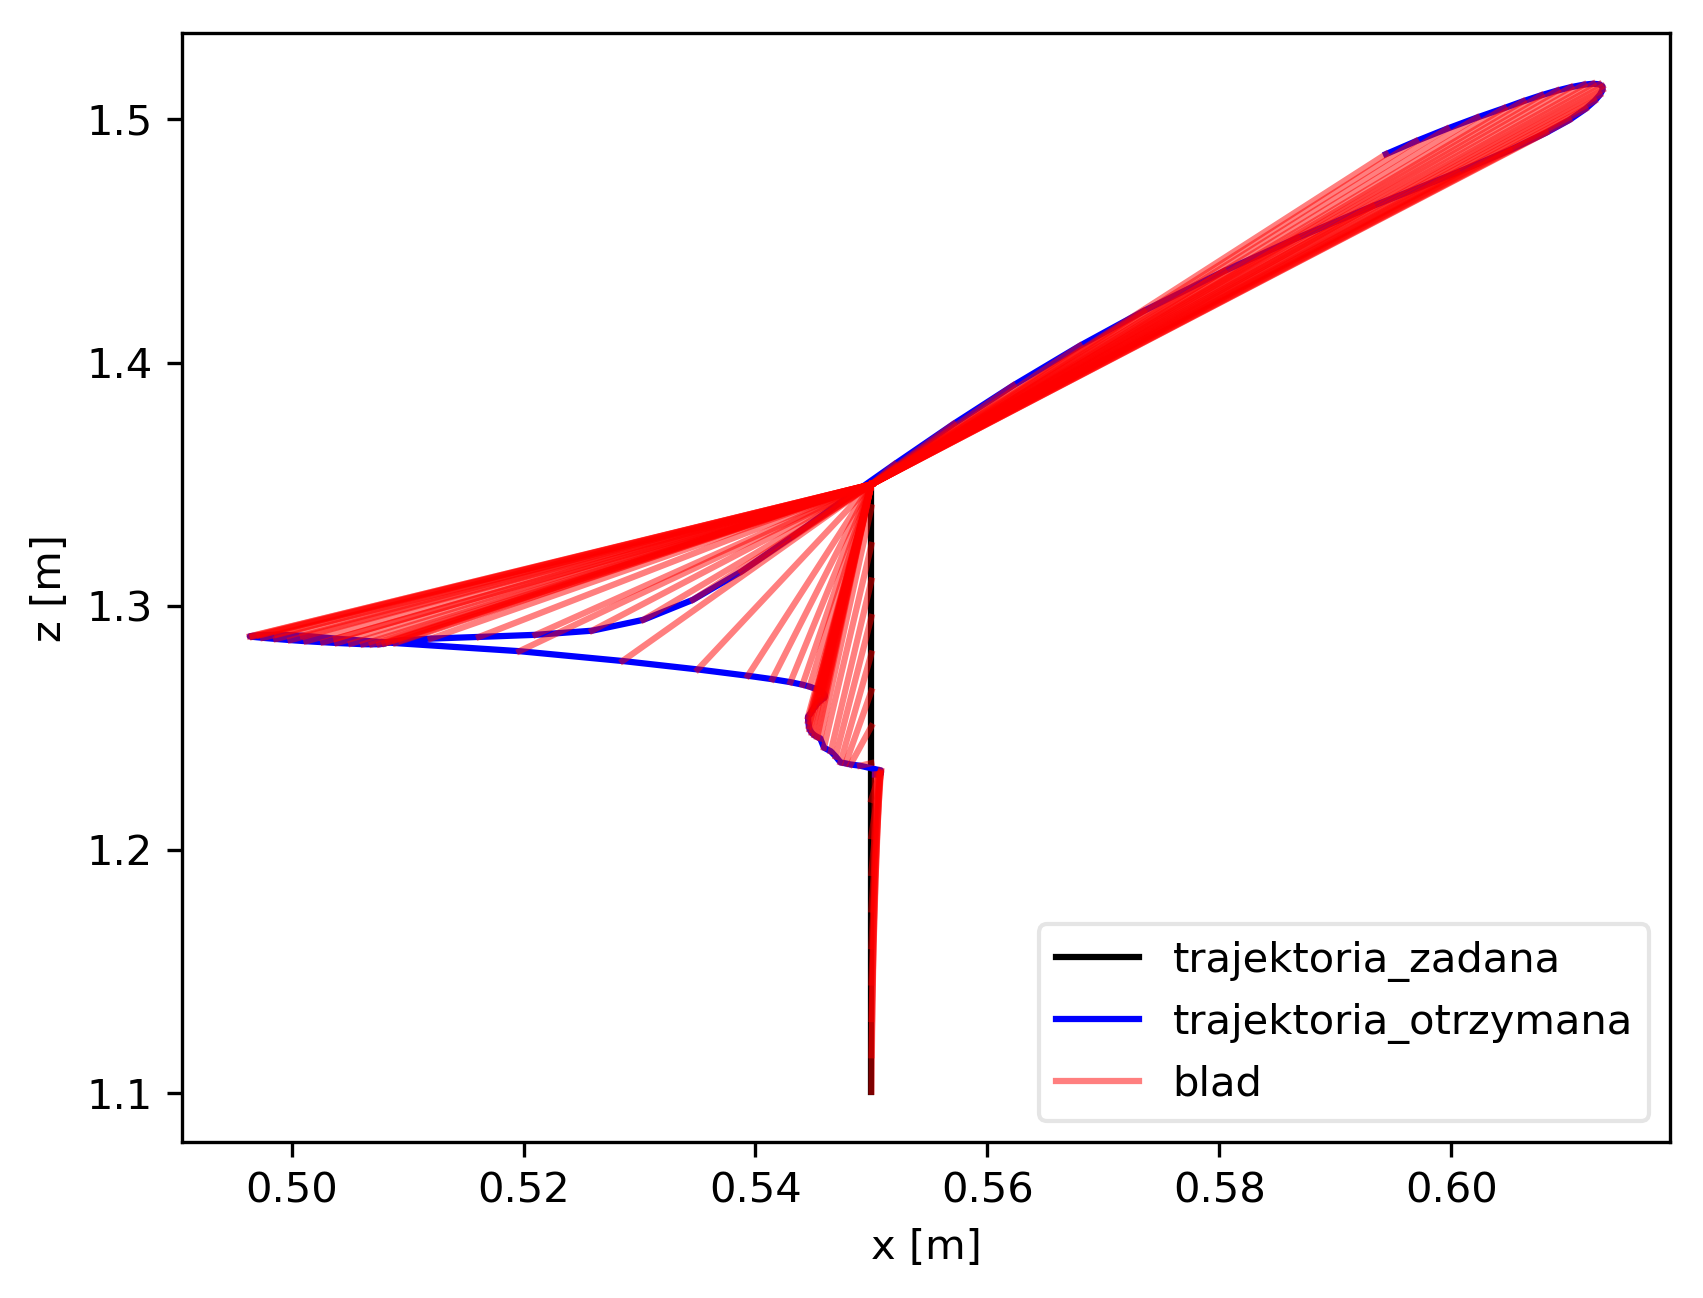
\includegraphics[width=.45\textwidth]{../../velma/przerobione_testy/out/podn/xz_ate_plot_podnoszenie_miekki_komp_wiertarka.png}
	}
	\caption{Podnoszenie przedmiotu. Porównanie trajektorii chwytaka w~osiach $X$ i~$Z$}
	\label{fig:podn_porow_przedm_bok}
\end{figure}

% \begin{figure}[H]
% 	\centering
% 	\subfigure[Rzut na wprost]{
% 		\label{fig:podn_porow_zbiorcze_a}
% 		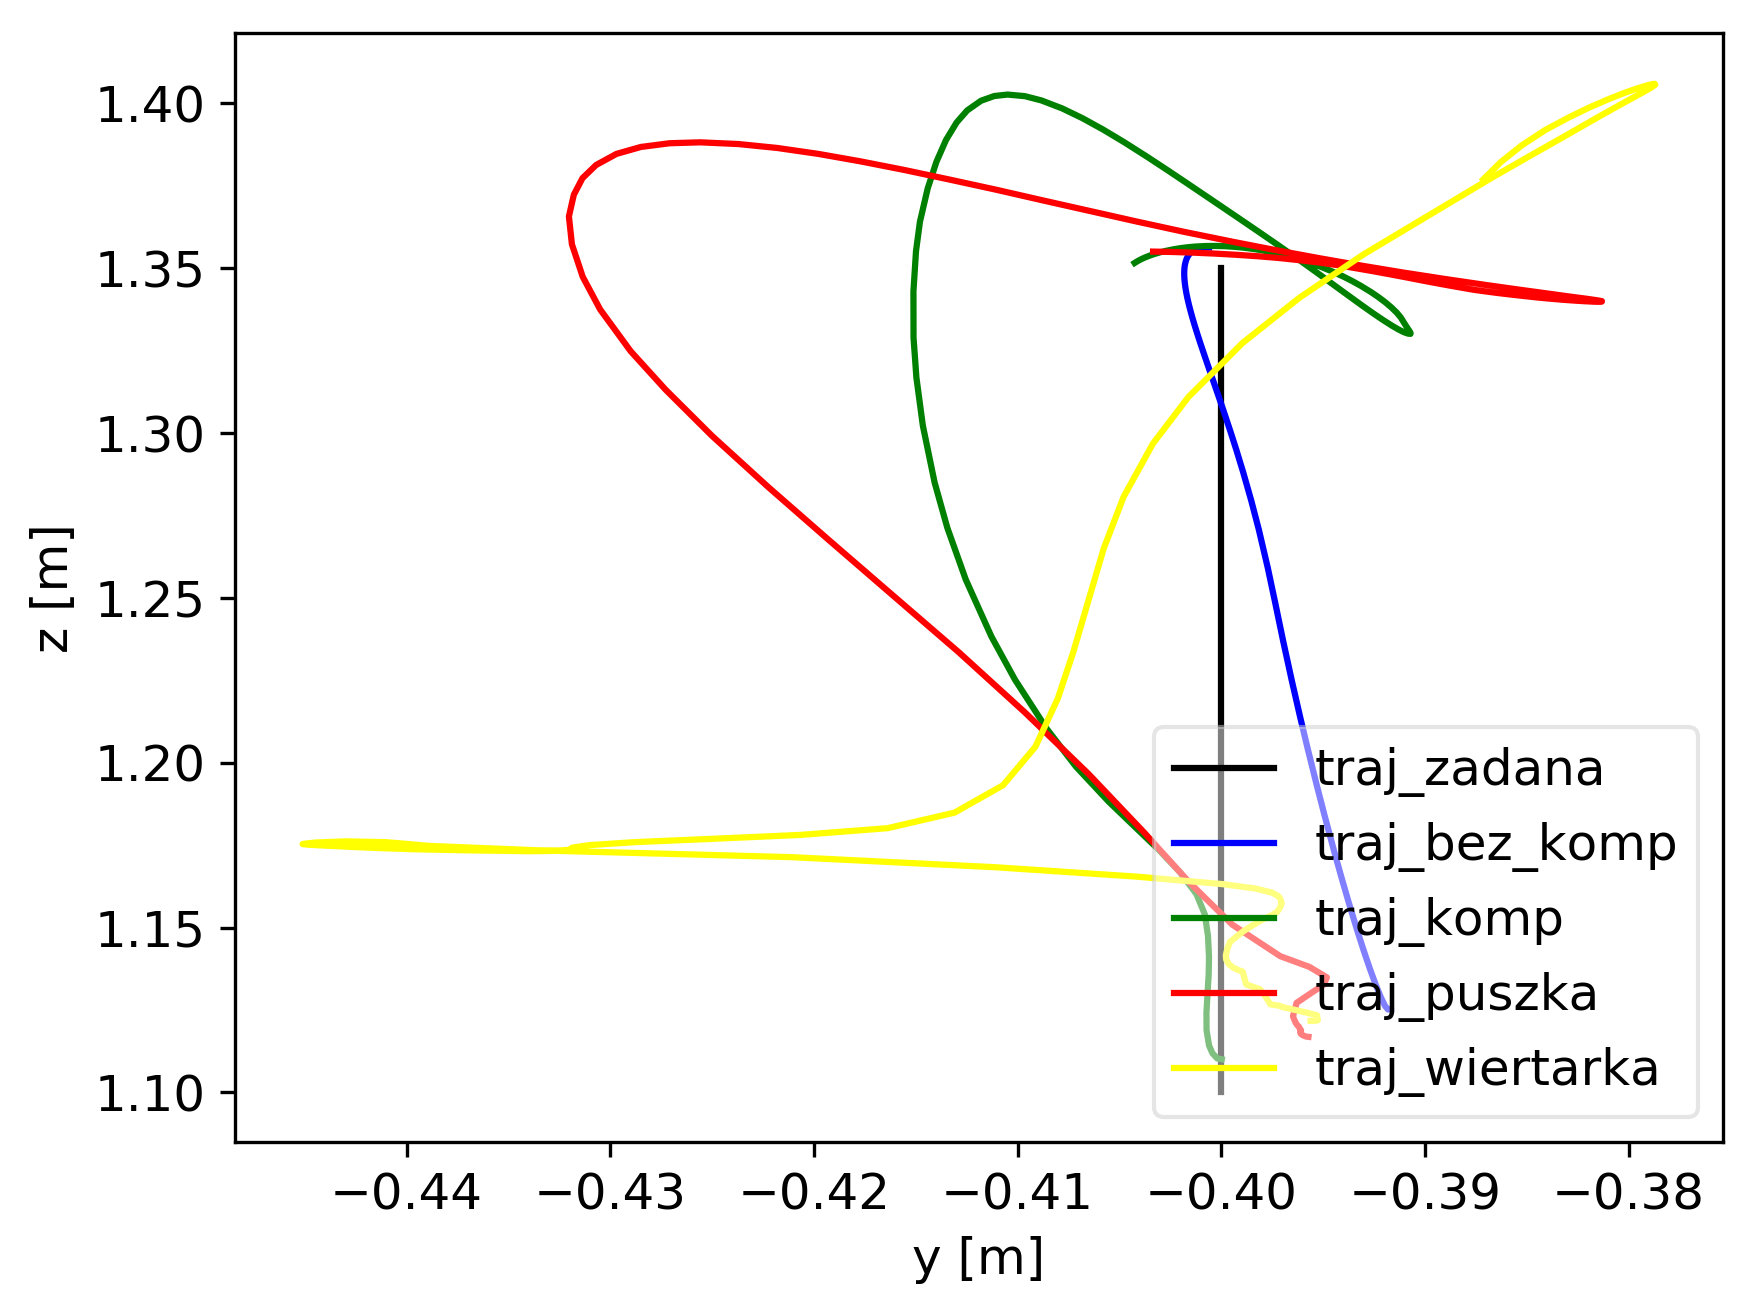
\includegraphics[width=.45\textwidth]{../../velma/przerobione_testy/out/podn/common_yz.png}
% 	}
% 	\hfill
% 	\subfigure[Rzut z~boku]{
% 		\label{fig:podn_porow_zbiorcze_b}
% 		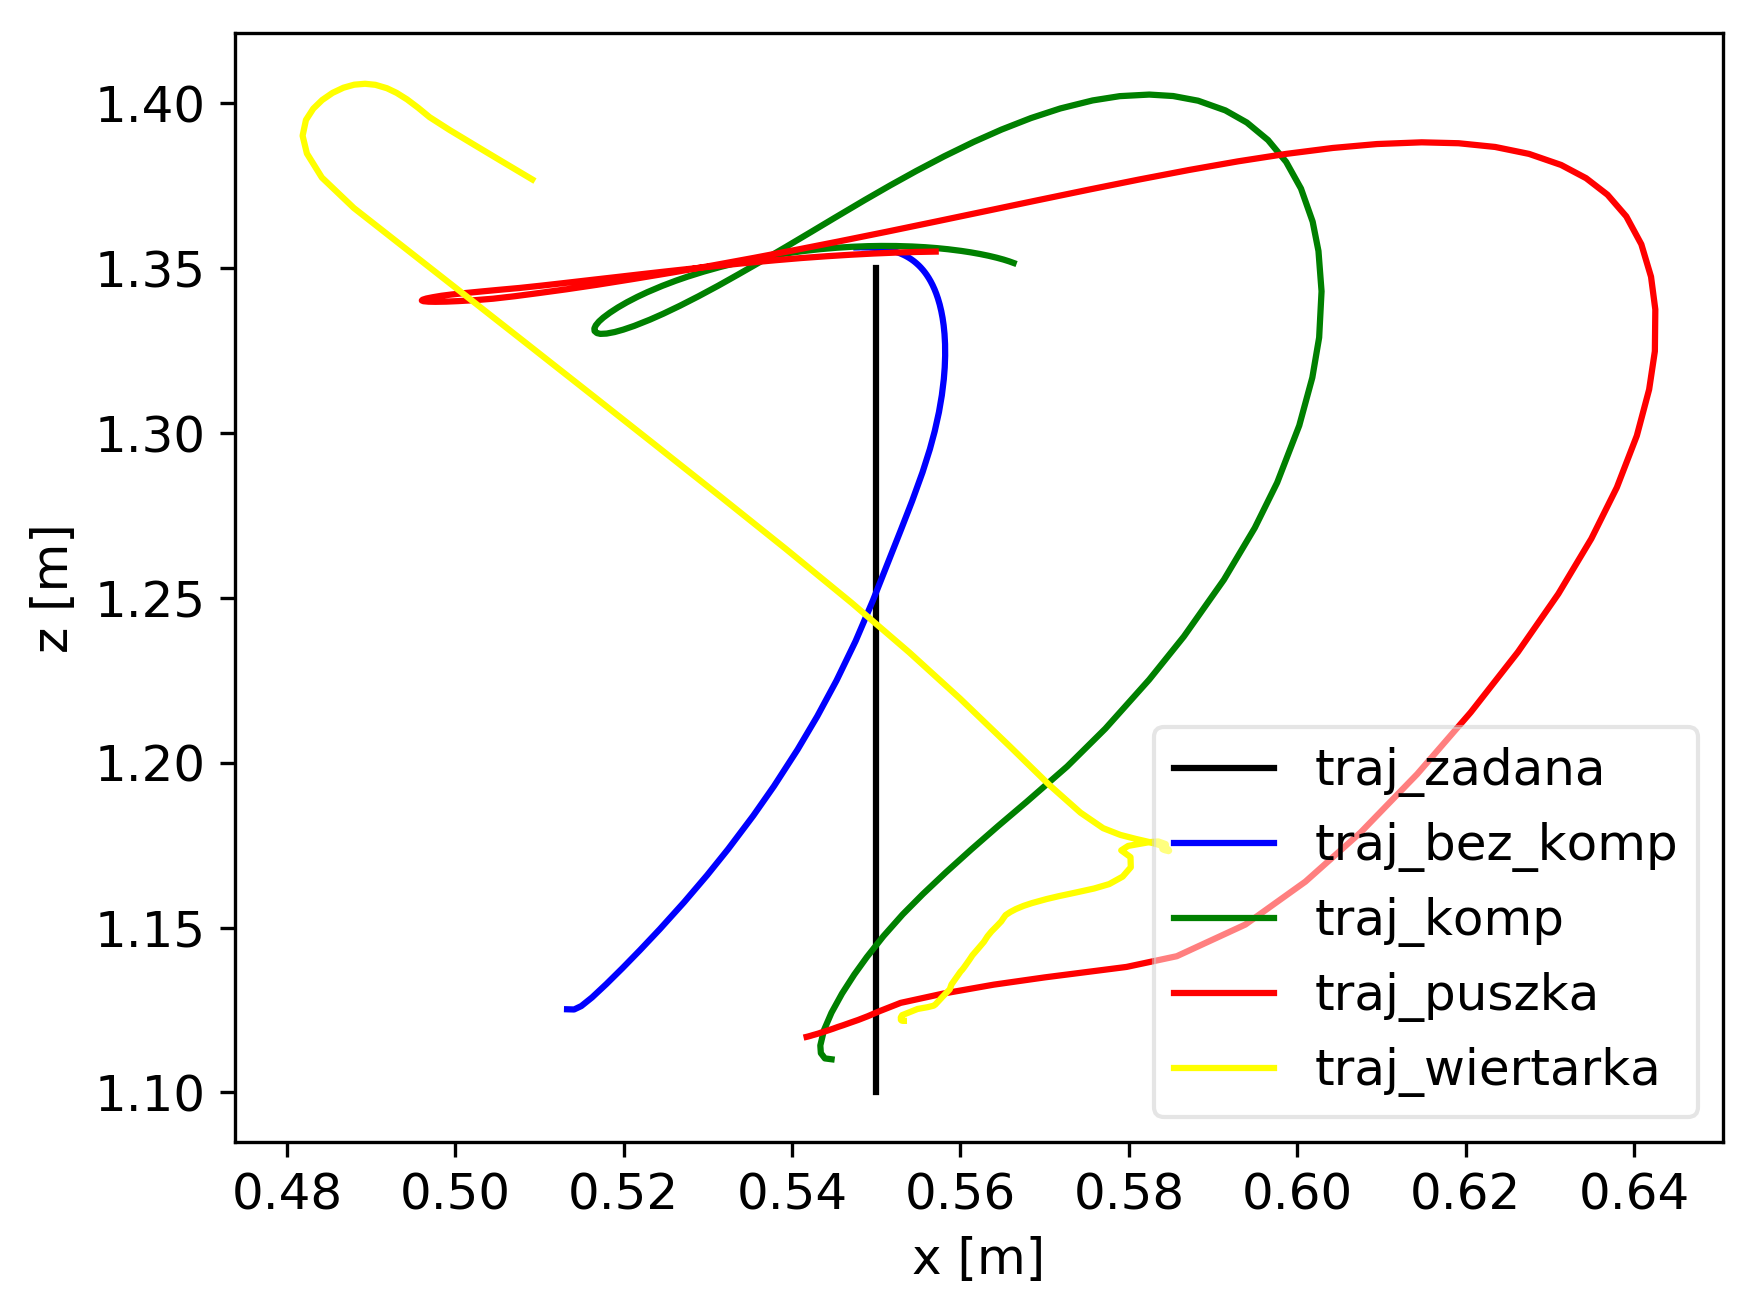
\includegraphics[width=.45\textwidth]{../../velma/przerobione_testy/out/podn/common_xz.png}
% 	}
% 	\caption{Porównanie wszystkich trajektorii bez zaznaczonego błędu}
% 	\label{fig:podn_porow_zbiorcze}
% \end{figure}




\section{Ruch ósemkowy}
Eksperyment ma przetestować zachowanie algorytmu kompensacji przy skomplikowanych ruchach (rys. \ref{fig:osemka_a}, \ref{fig:osemka_rot}).  Ruch ósemkowy" zadany jest w~osi $Y$ oraz $Z$.
Trajektoria jest zadana zgodnie ze wzorem lemniskaty Bernoullego opisanej wzorem:
\begin{equation}
(y^2 + z^2)^2 = 2a^2(y^2-z^2)
\end{equation}

gdzie:
\begin{itemize}
	\item $y$ oraz $z$ to współrzędne trajektorii
	\item $a$ to parametr równania
\end{itemize}

Trajektoria ruchu w~rzucie ATE ruchu została zaprezentowana na rys. \ref{fig:osemka_porow_komp} i~\ref{fig:osemka_porow_przedm}. Trajektoria widoczna z~boku (w osiach $X$ oraz $Z$) została zaprezentowana na rys. \ref{fig:osemka_porow_komp_bok}, \ref{fig:osemka_porow_przedm_bok}.
\begin{figure}[H]
	\centering
	\subfigure[Oś $X$]{
		\label{fig:osemka_ax}
		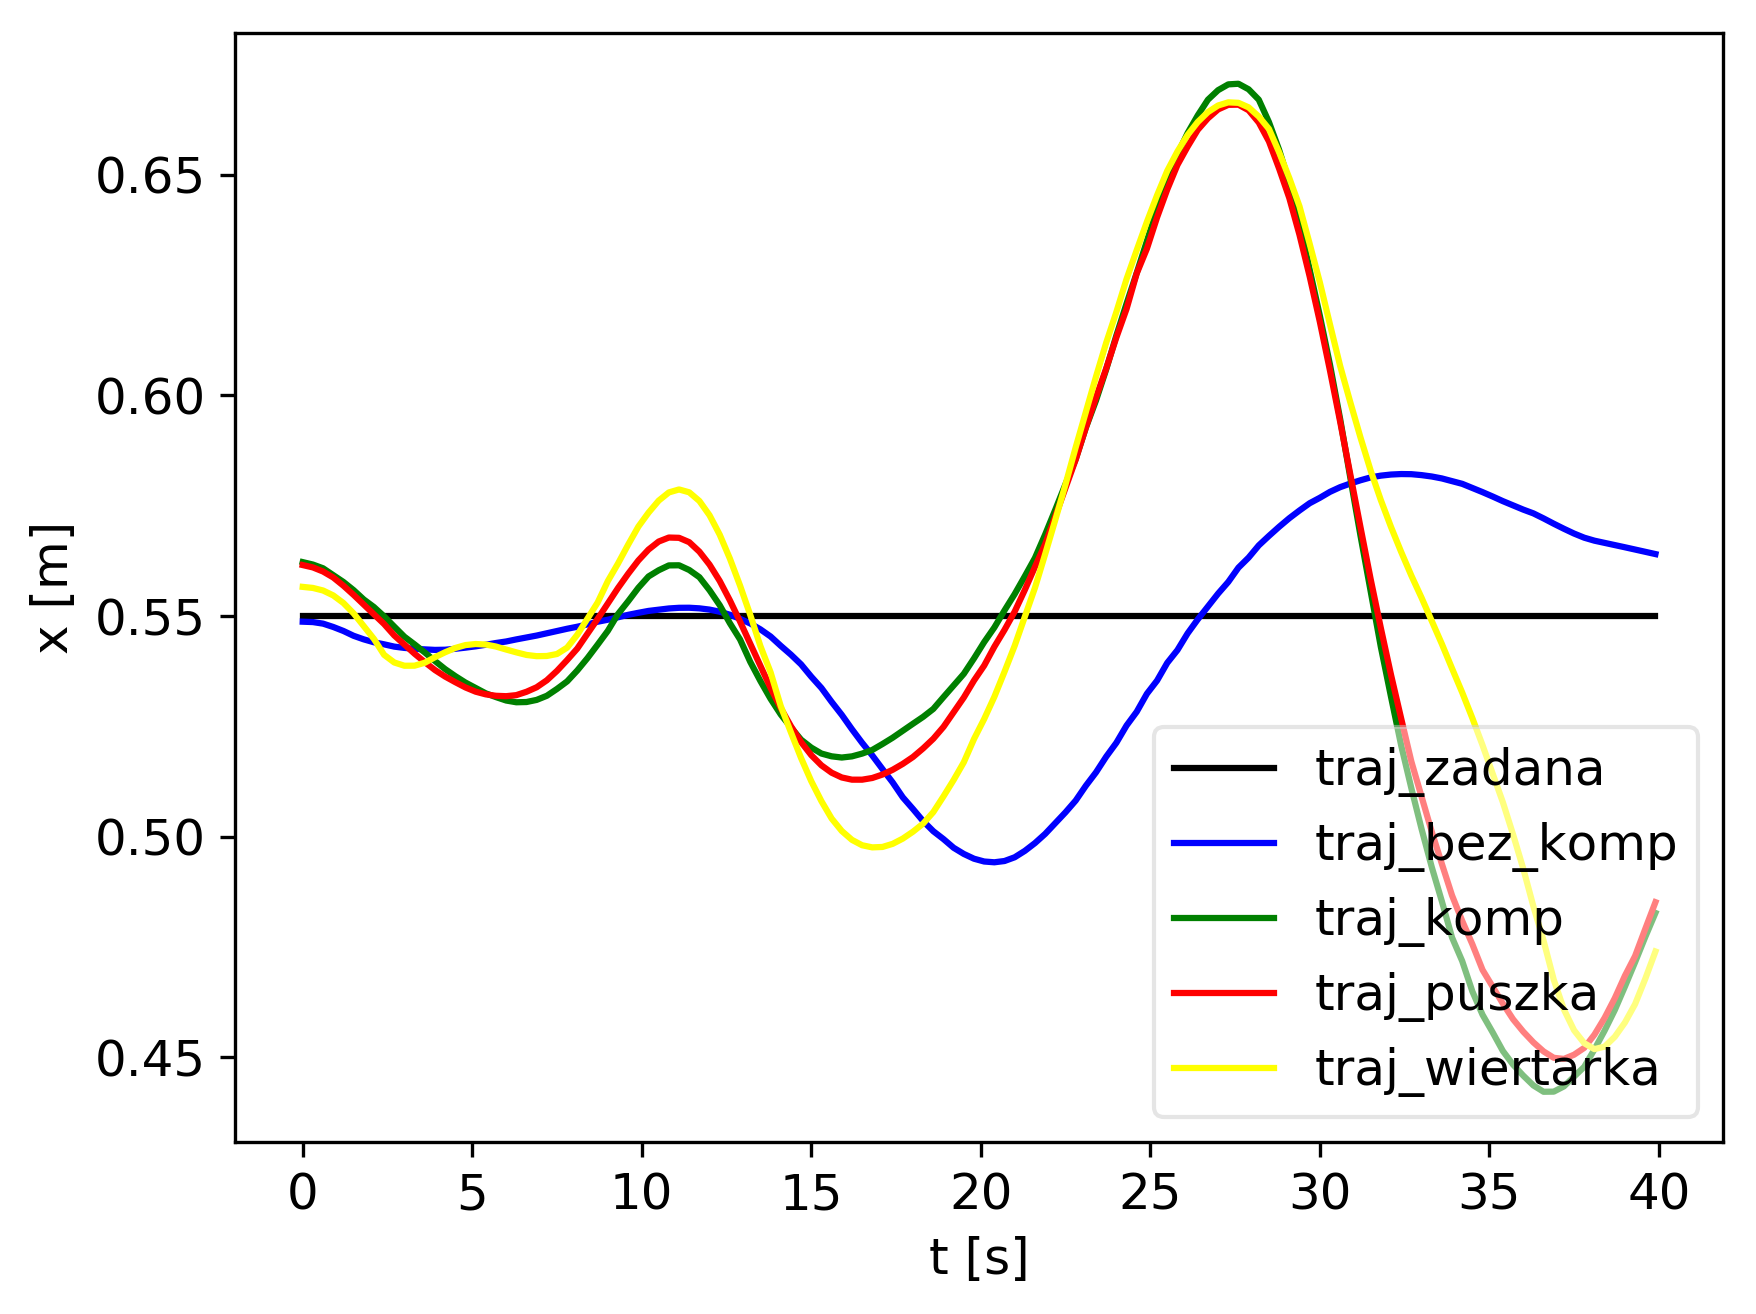
\includegraphics[width=.45\textwidth]{../../velma/przerobione_testy/out/osemka/common_ax.png}
	}
	\hfill
	\subfigure[Oś $Y$]{
		\label{fig:osemka_ay}
		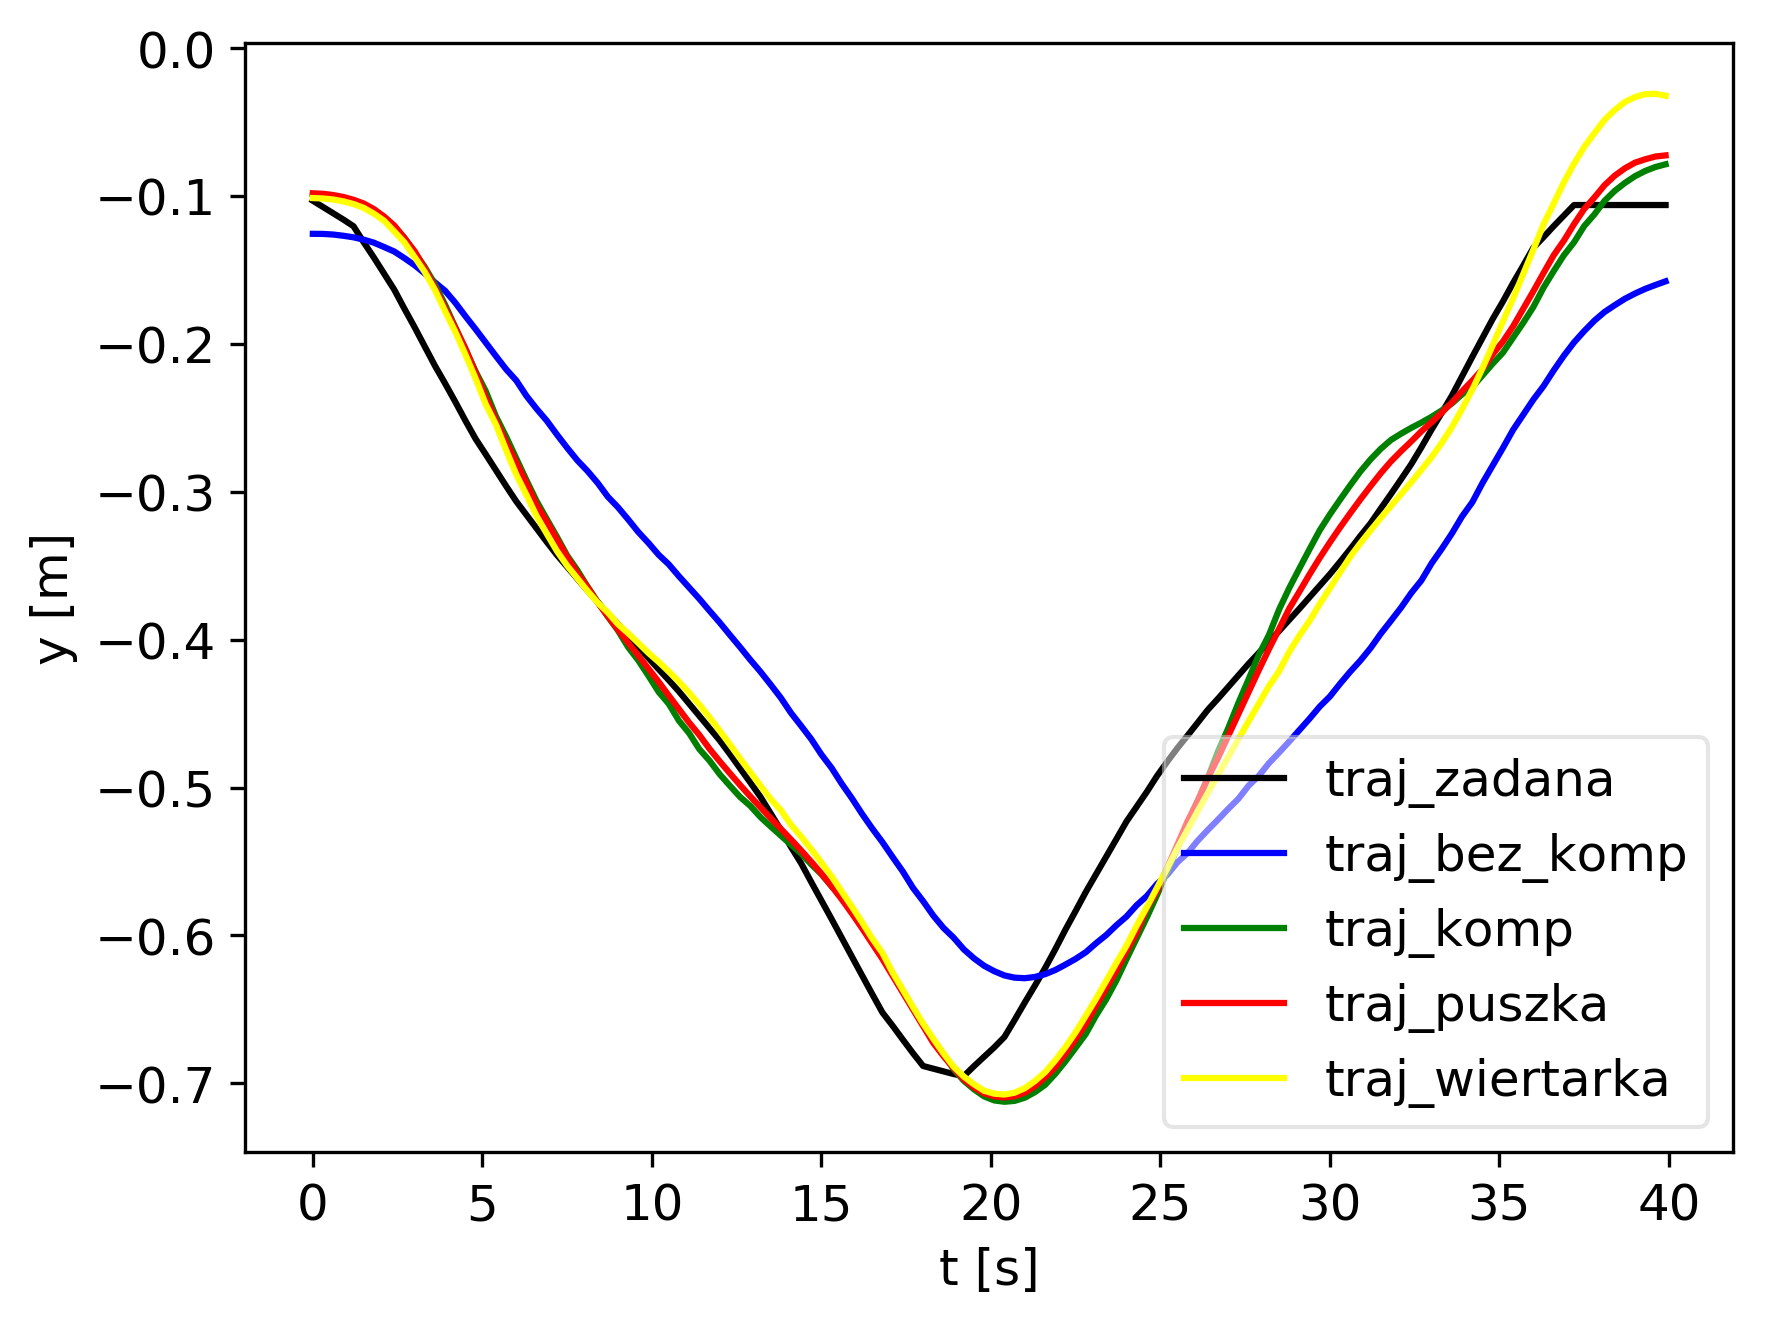
\includegraphics[width=.45\textwidth]{../../velma/przerobione_testy/out/osemka/common_ay.png}
	}
	
	
	\subfigure[Oś $Z$]{
		\label{fig:osemka_az}
		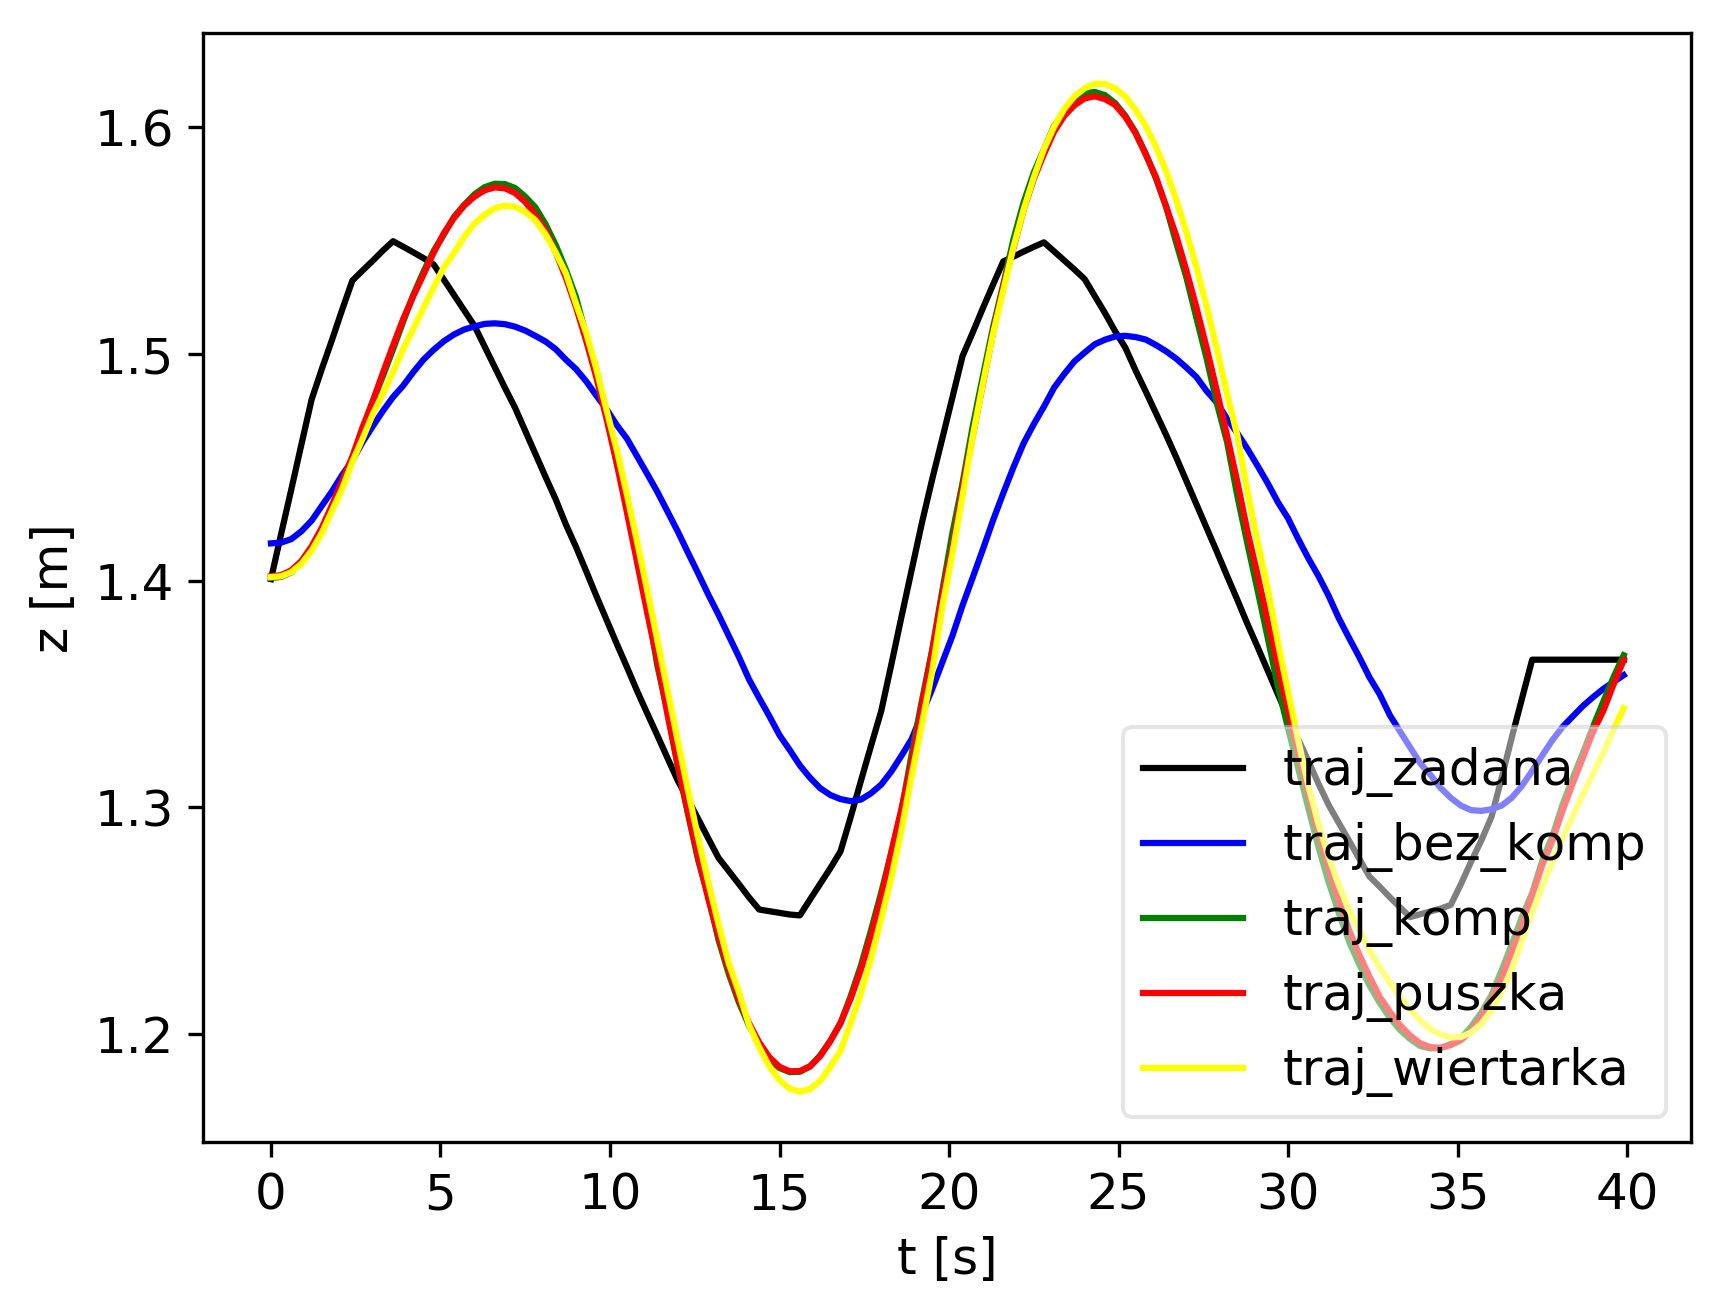
\includegraphics[width=.45\textwidth]{../../velma/przerobione_testy/out/osemka/common_az.png}
	}

	\caption{Ruch ósemkowy. Porównanie trajektorii pozycji w~zależności od czasu.}
	\label{fig:osemka_a}

\end{figure}

\begin{figure}[H]
	\centering
	\subfigure[Brak algorytmu kompensacji]{
		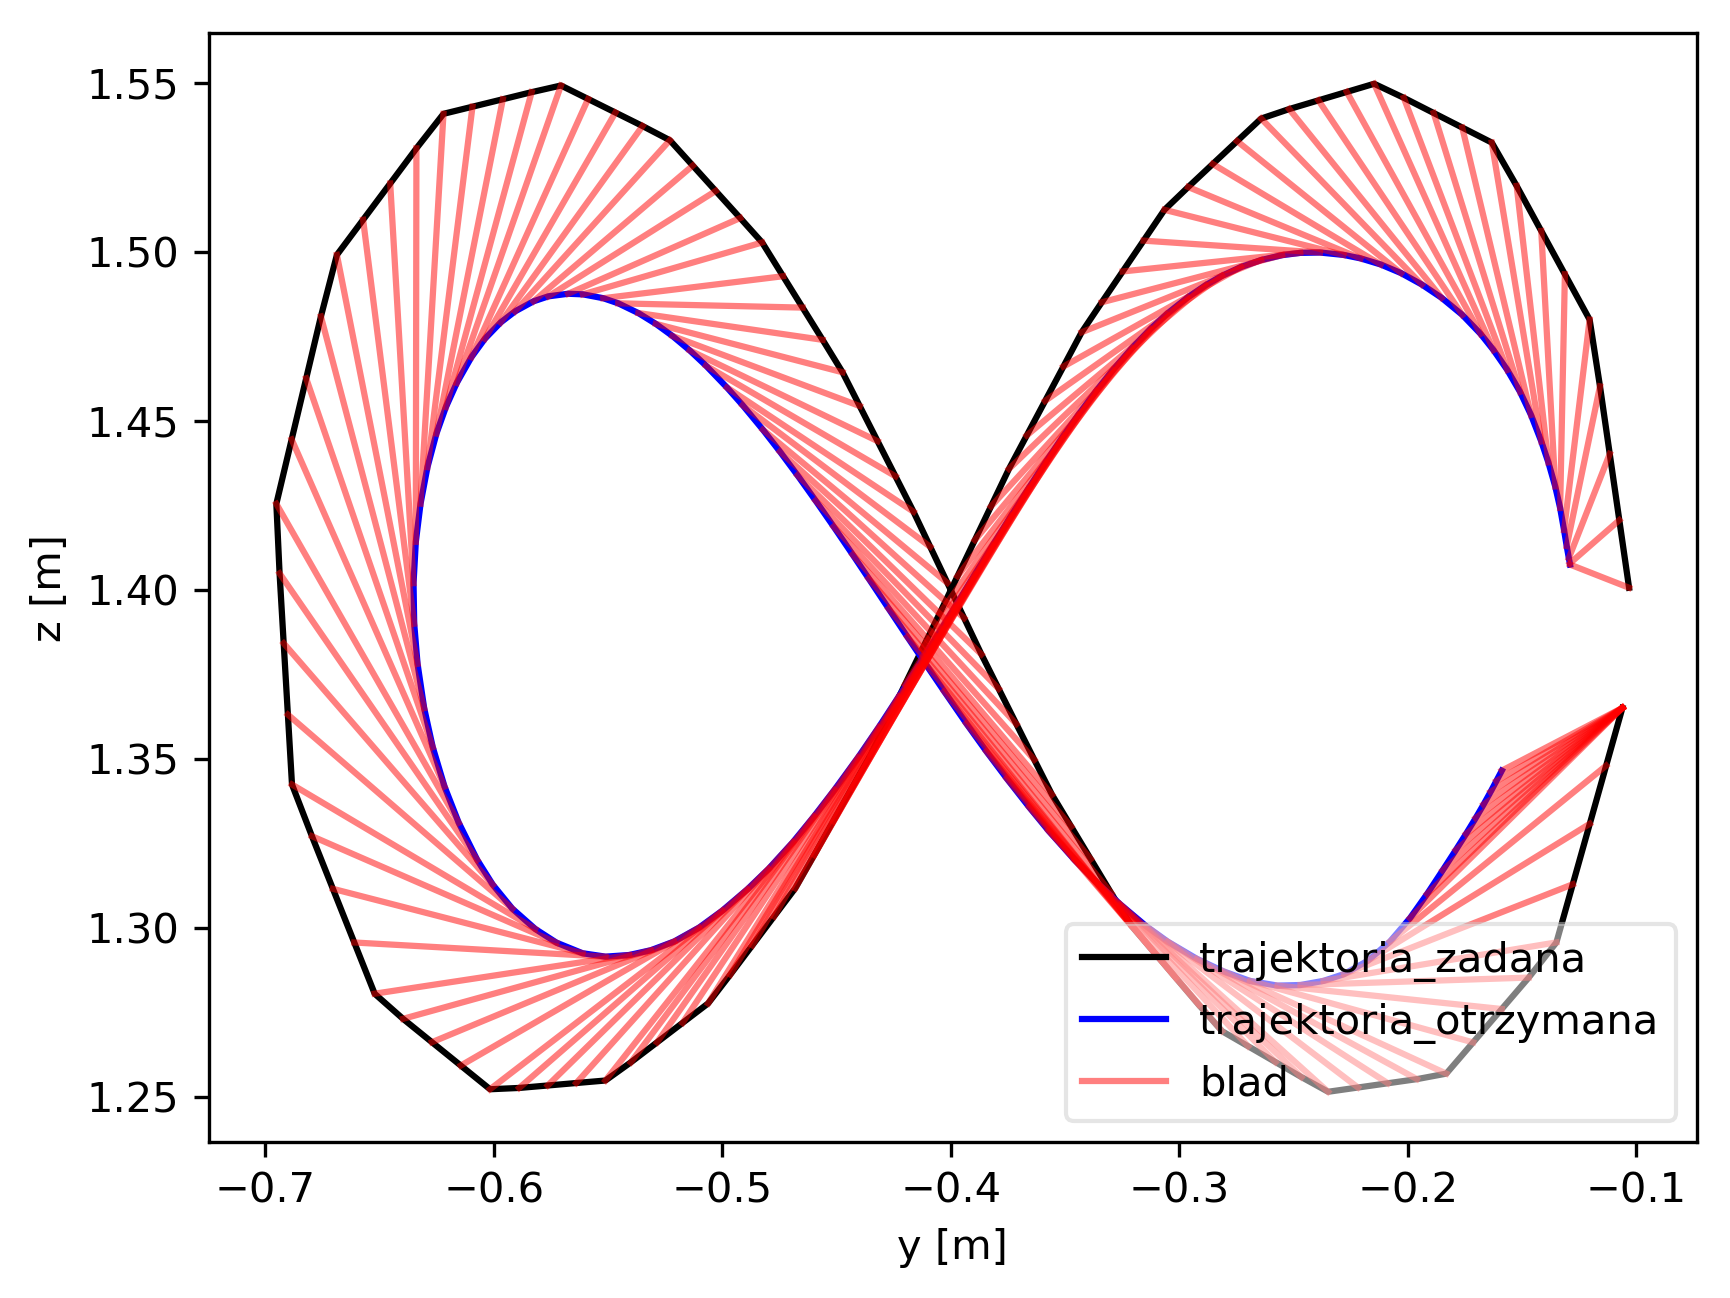
\includegraphics[width=.45\textwidth]{../../velma/przerobione_testy/out/osemka/yz_ate_plot_podnoszenie_miekki_bez_brak.png}
	}
	\hfill
	\subfigure[Zalaczony algorytm kompnesacji]{
		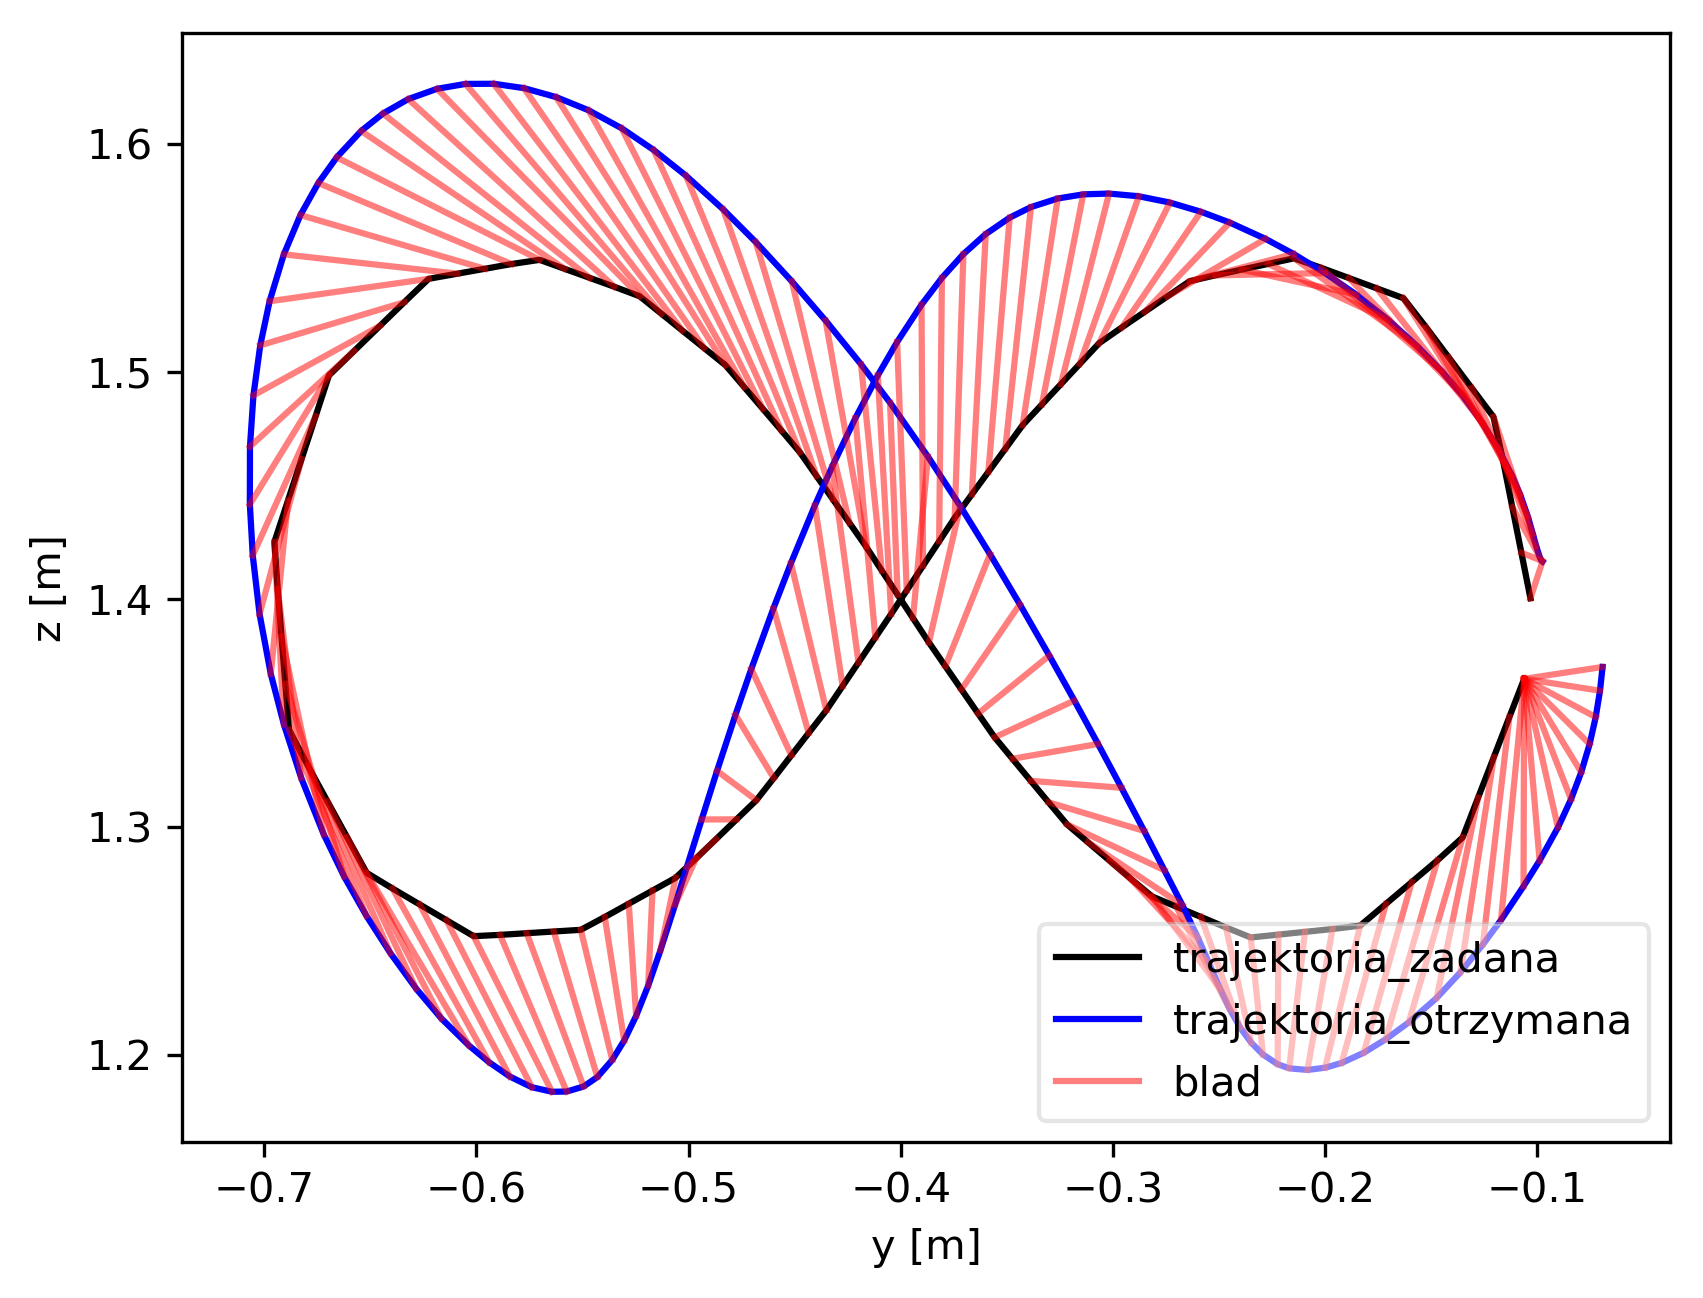
\includegraphics[width=.45\textwidth]{../../velma/przerobione_testy/out/osemka/yz_ate_plot_podnoszenie_miekki_komp_brak.png}
	}
	\caption{Porównanie trajektorii chwytaka w~osiach $Y$ i~$Z$}
	\label{fig:osemka_porow_komp}
\end{figure}


\begin{figure}[H]
	\centering
	\subfigure[Kąt osi $X$]{
		\label{fig:osemka_rotx}
		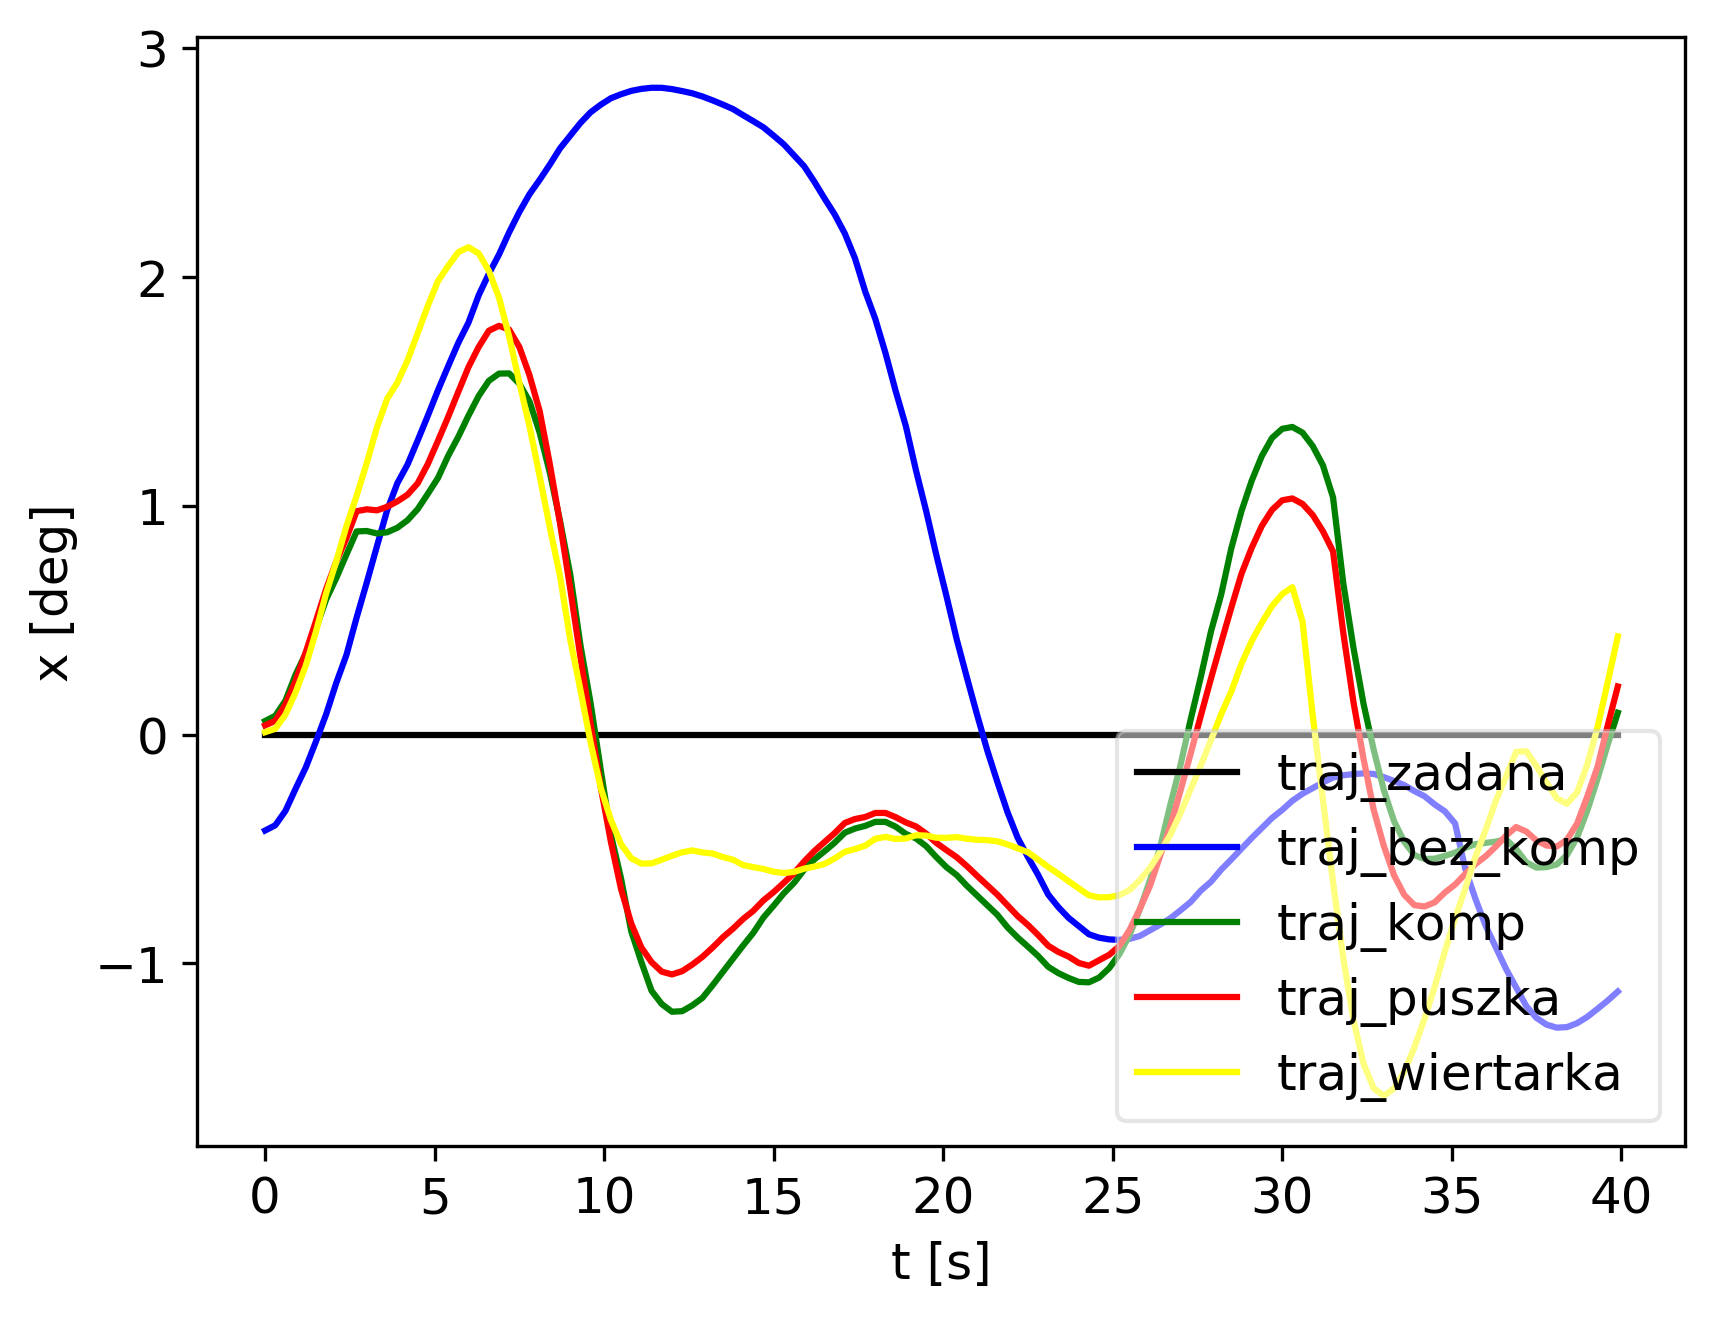
\includegraphics[width=.45\textwidth]{../../velma/przerobione_testy/out/osemka/common_rotx.png}
	}
	\hfill
	\subfigure[Kąt osi $Y$]{
		\label{fig:do_gory_roty}
		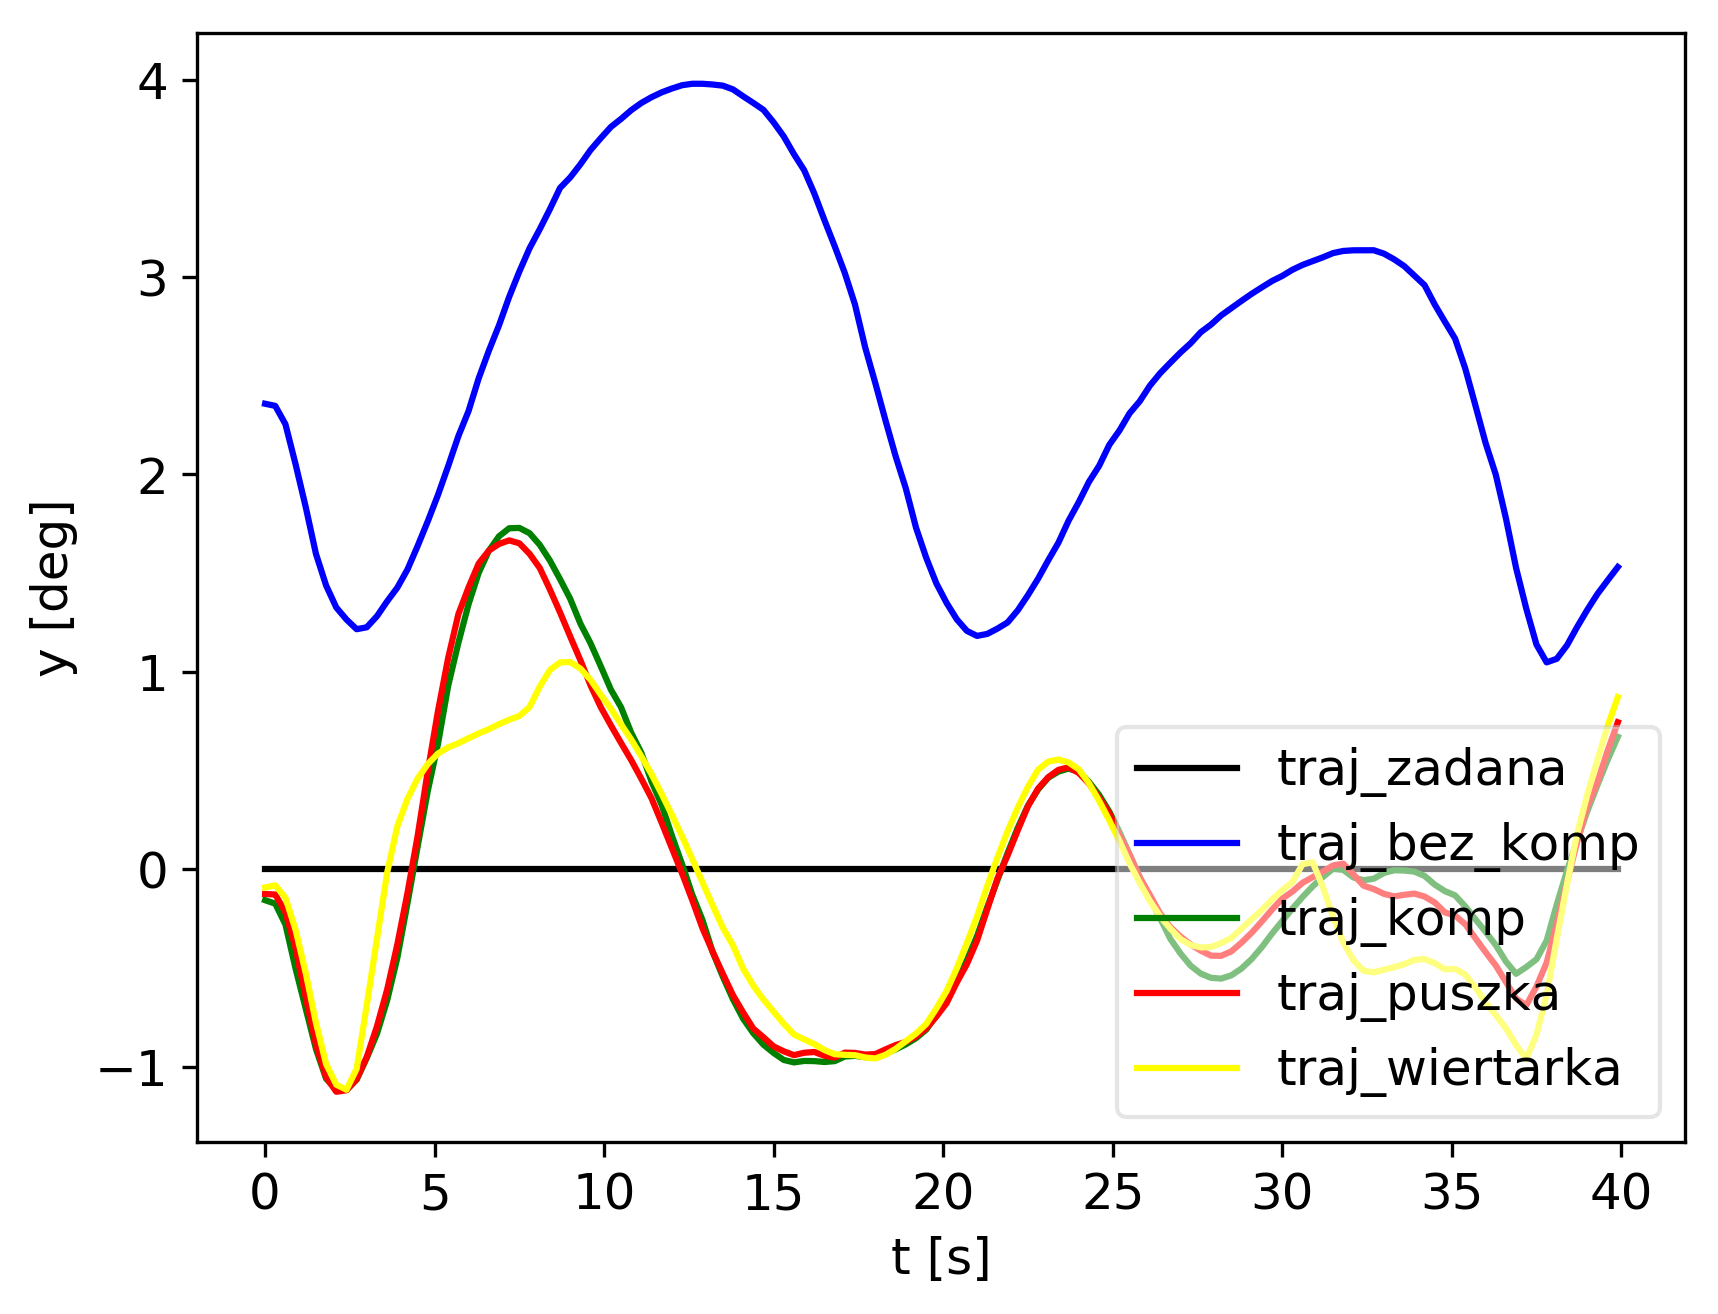
\includegraphics[width=.45\textwidth]{../../velma/przerobione_testy/out/osemka/common_roty.png}
	}
	
	
	\subfigure[Kąt osi $Z$]{
		\label{fig:osemka_rotz}
		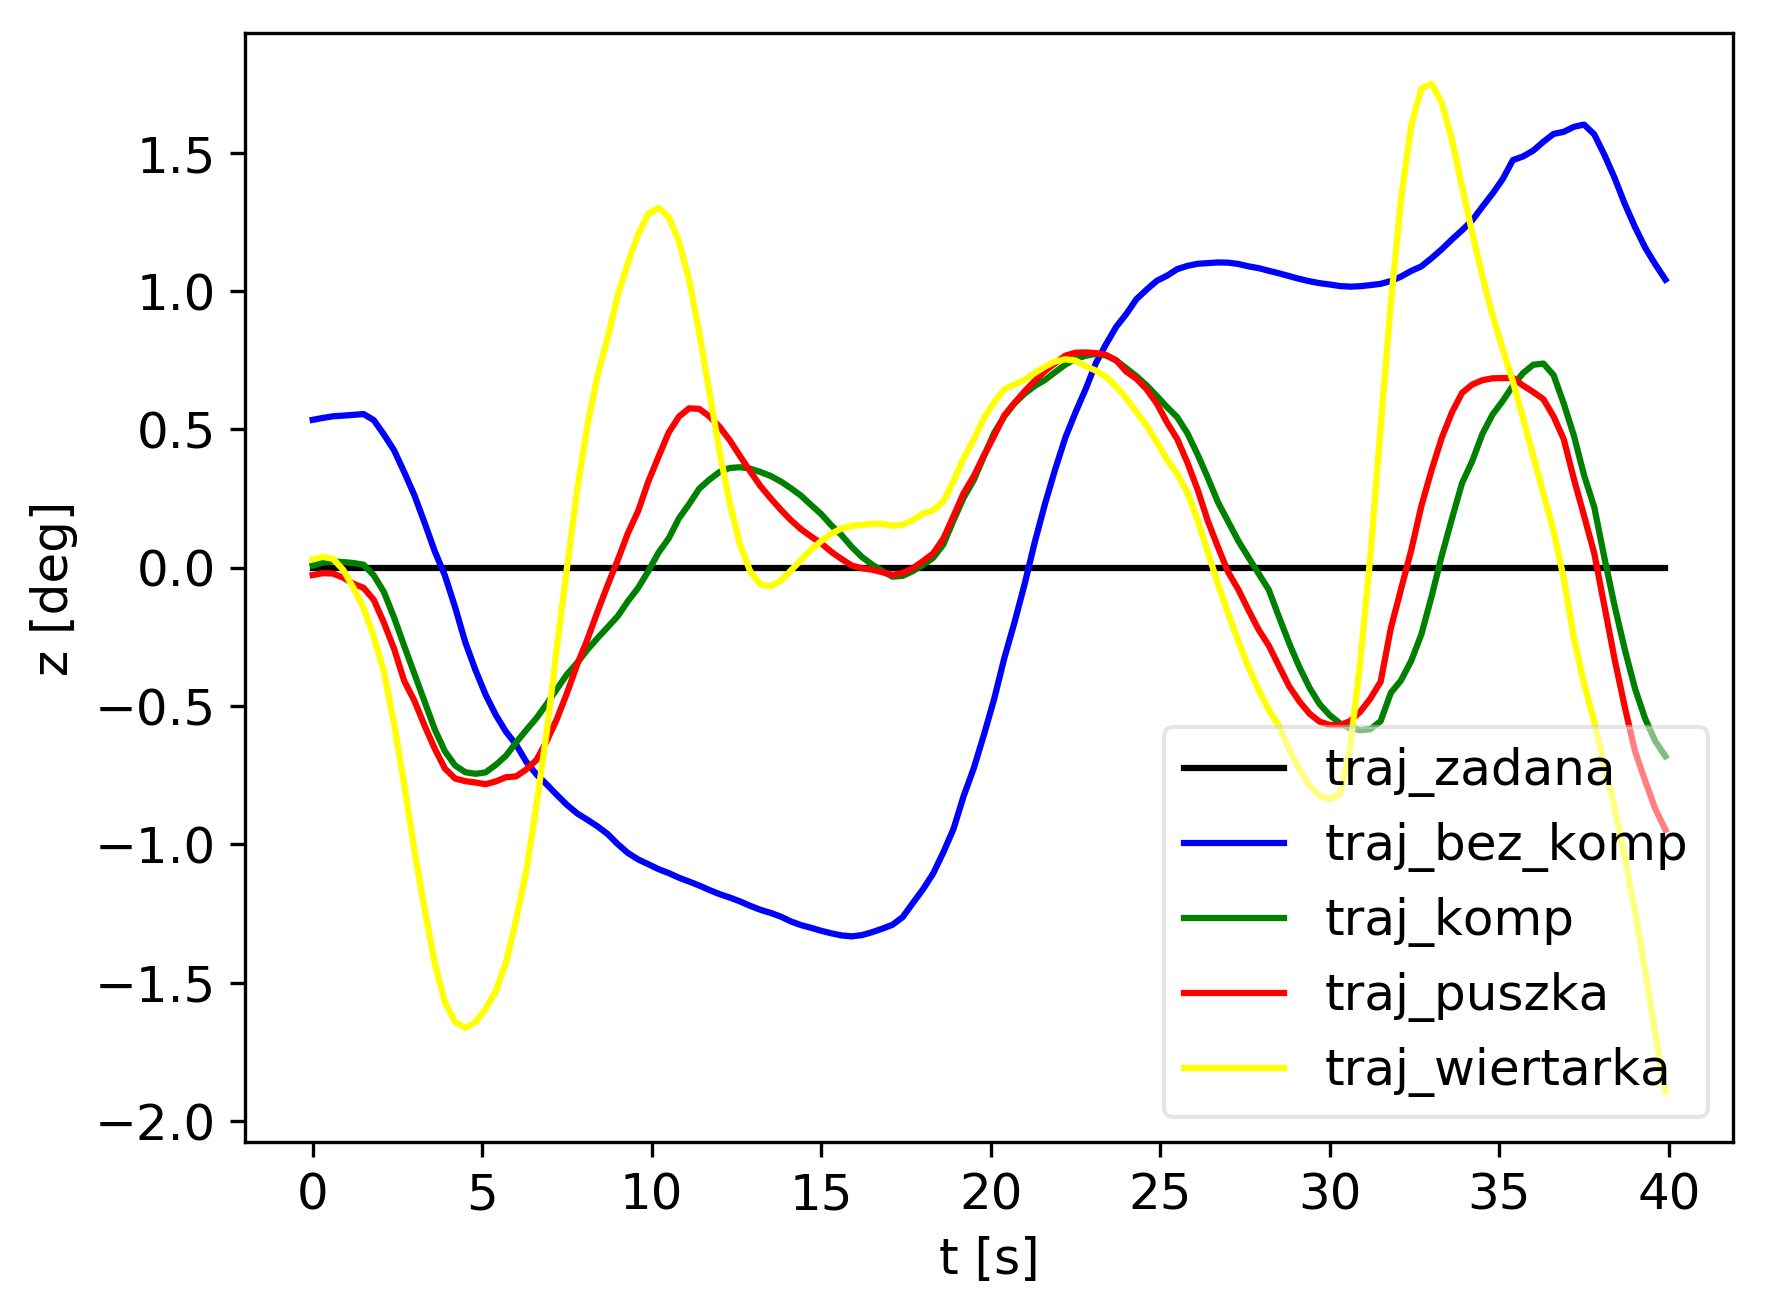
\includegraphics[width=.45\textwidth]{../../velma/przerobione_testy/out/osemka/common_rotz.png}
	}

	\caption{Ruch ósemkowy. Porównanie trajektorii kątów w~notacji Eulera w~zależności od czasu.}
	\label{fig:osemka_rot}

\end{figure}


\begin{figure}[H]
	\centering
	\subfigure[Trajektoria z~chwycona puszka]{
		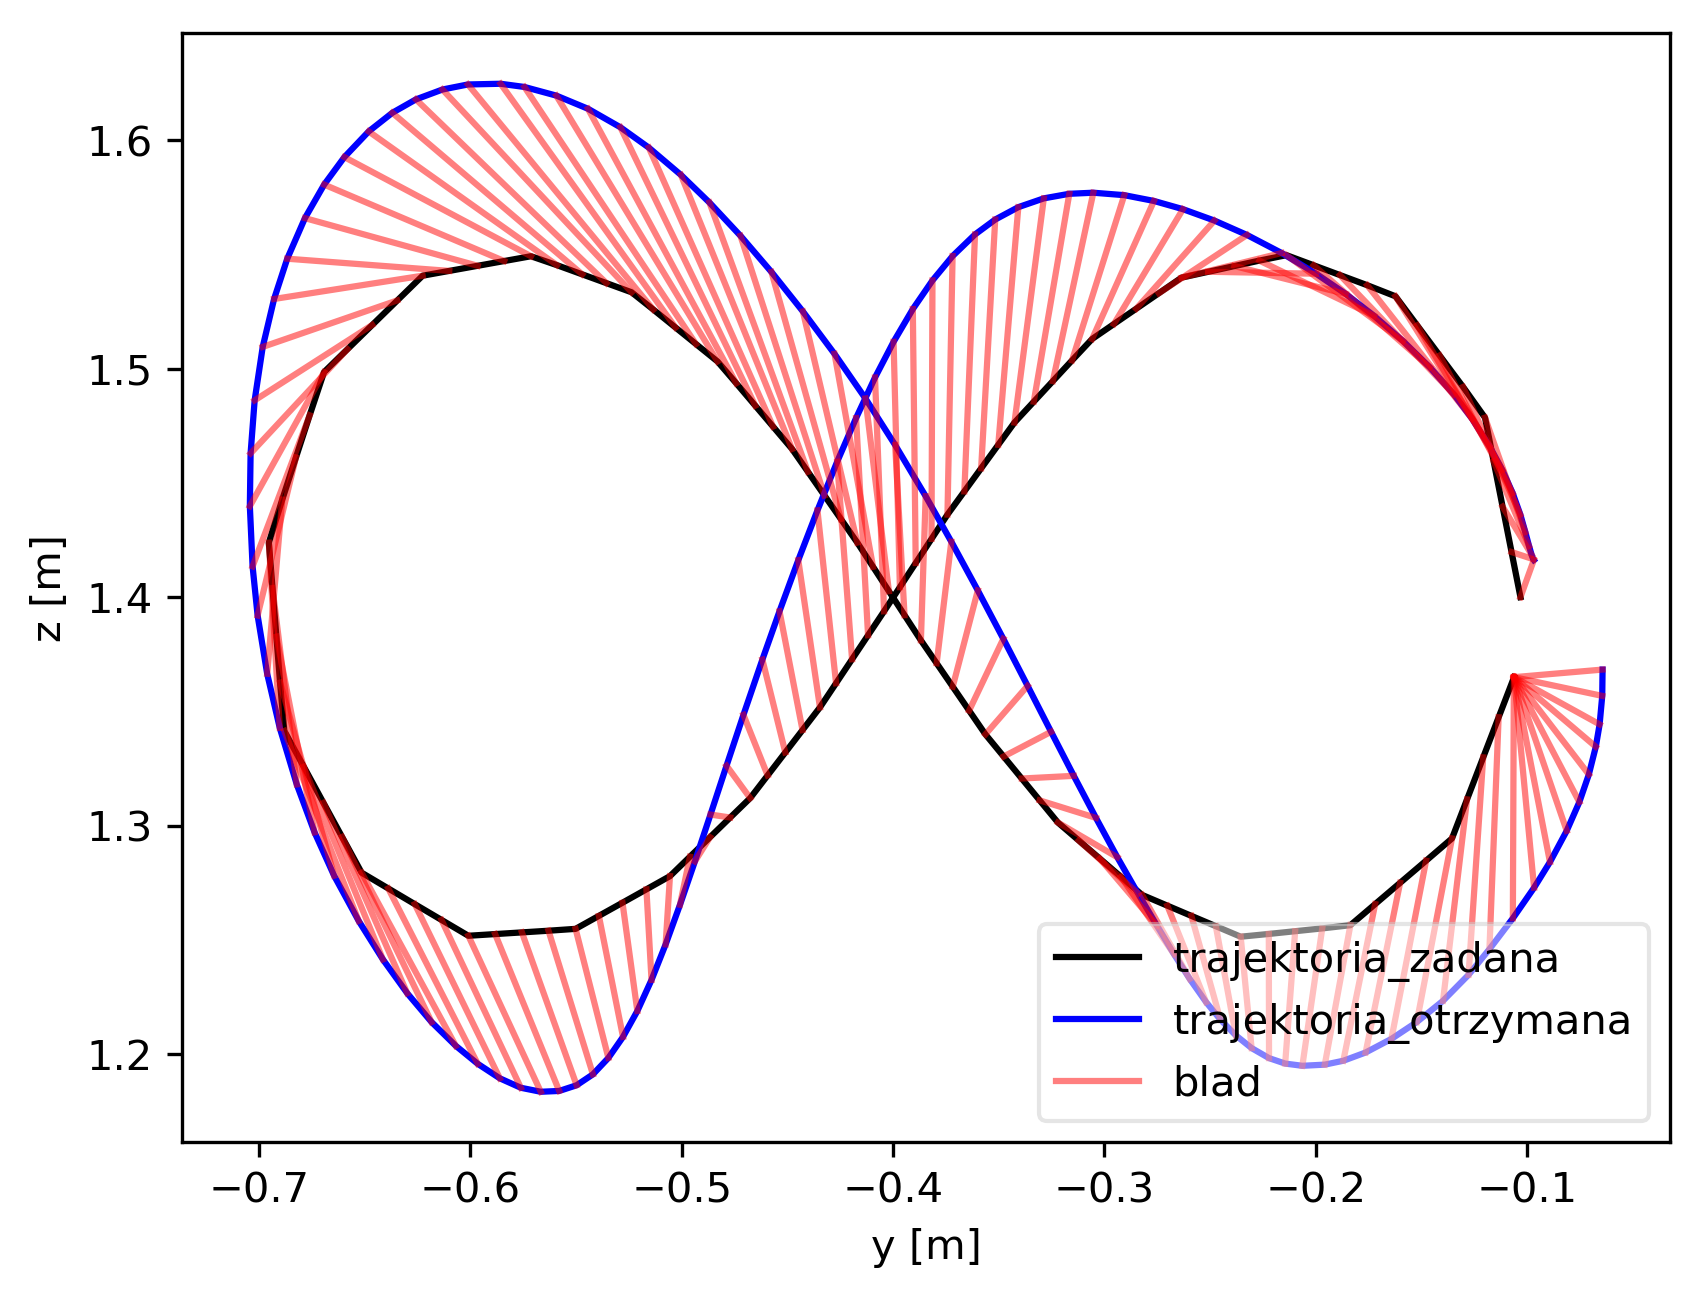
\includegraphics[width=.45\textwidth]{../../velma/przerobione_testy/out/osemka/yz_ate_plot_podnoszenie_miekki_komp_piwo.png}
	}
	\hfill
	\subfigure[Trajektoria z~chwycona wiertarka]{
		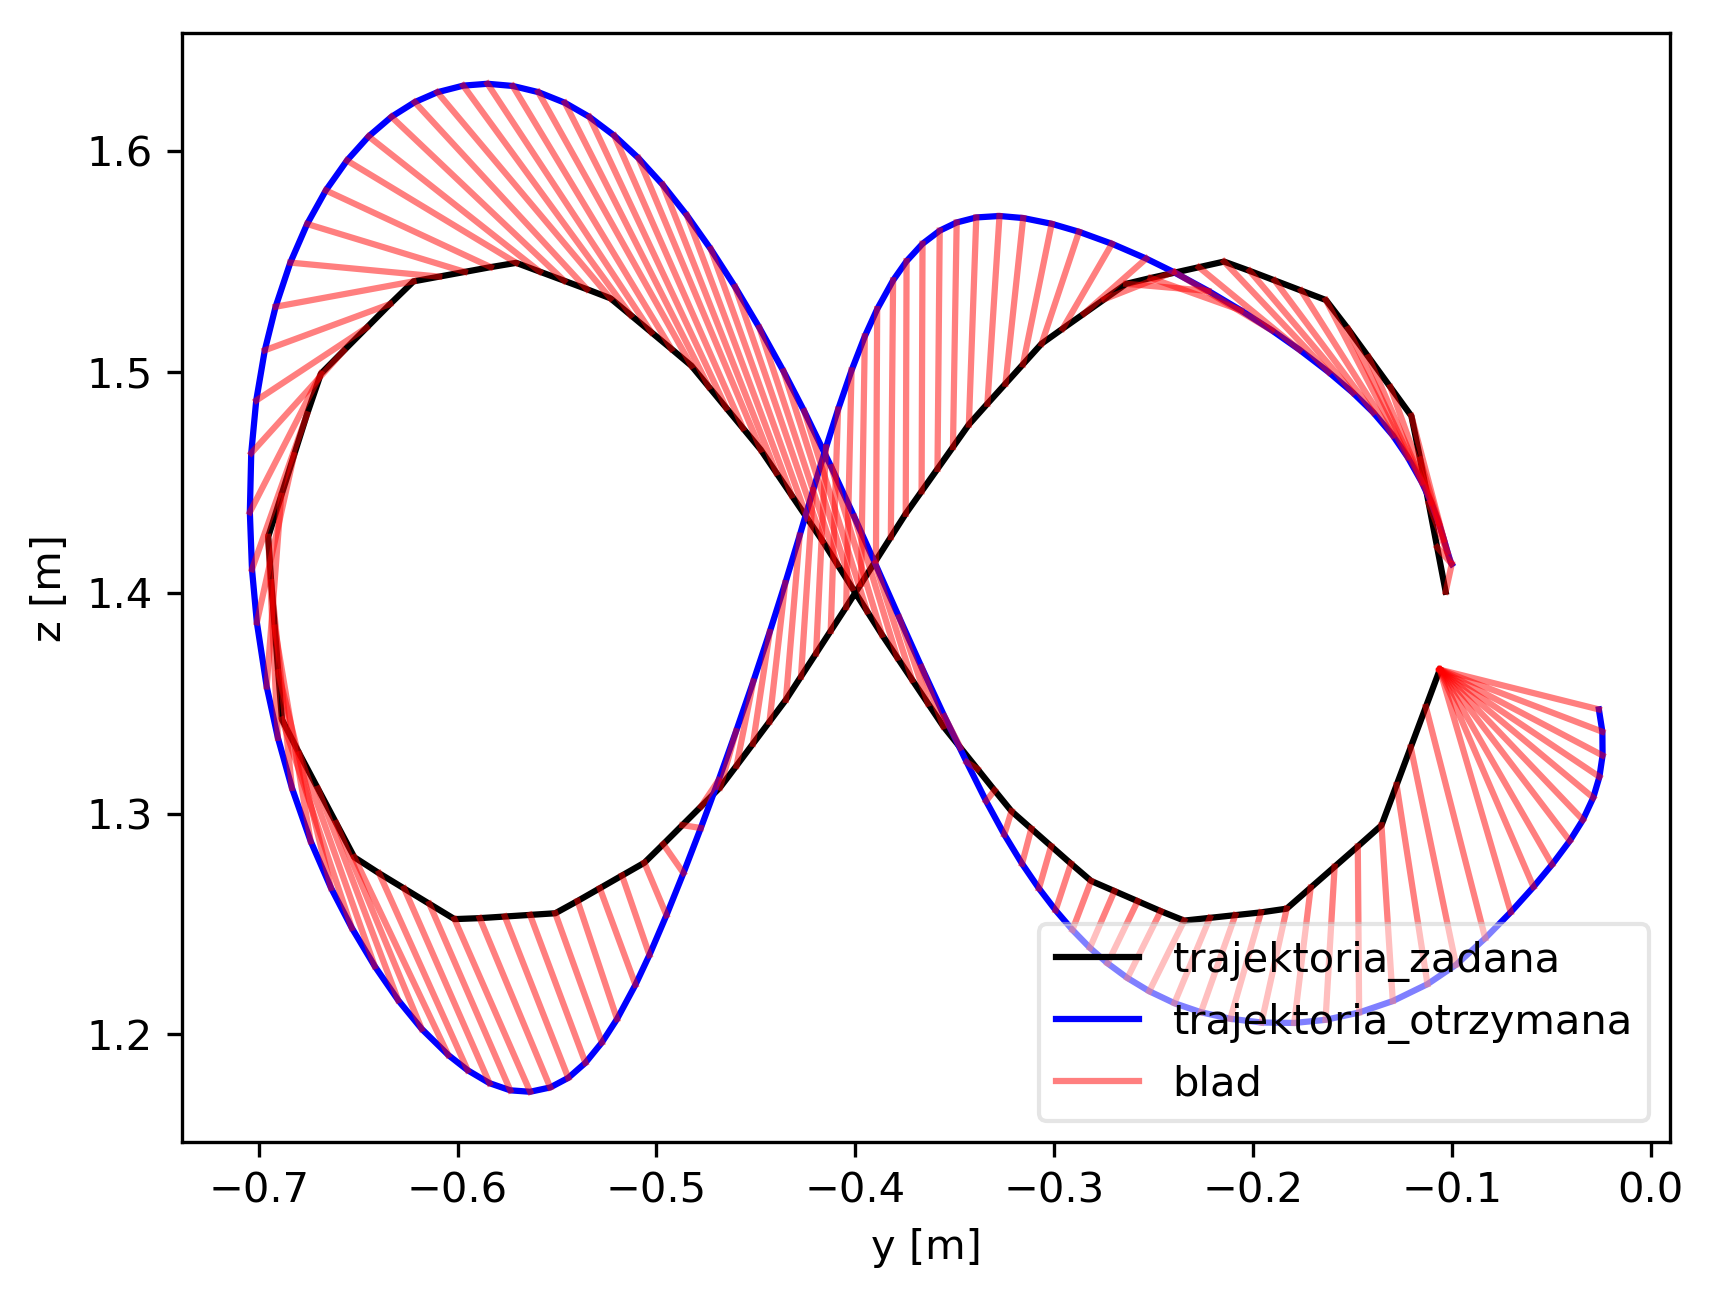
\includegraphics[width=.45\textwidth]{../../velma/przerobione_testy/out/osemka/yz_ate_plot_podnoszenie_miekki_komp_wiertarka.png}
	}
	\caption{Ruch ósemkowy. Porównanie trajektorii chwytaka w~osiach $Y$ i~$Z$}
	\label{fig:osemka_porow_przedm}
\end{figure}


\begin{figure}[H]
	\centering
	\subfigure[Brak algorytmu kompensacji]{
		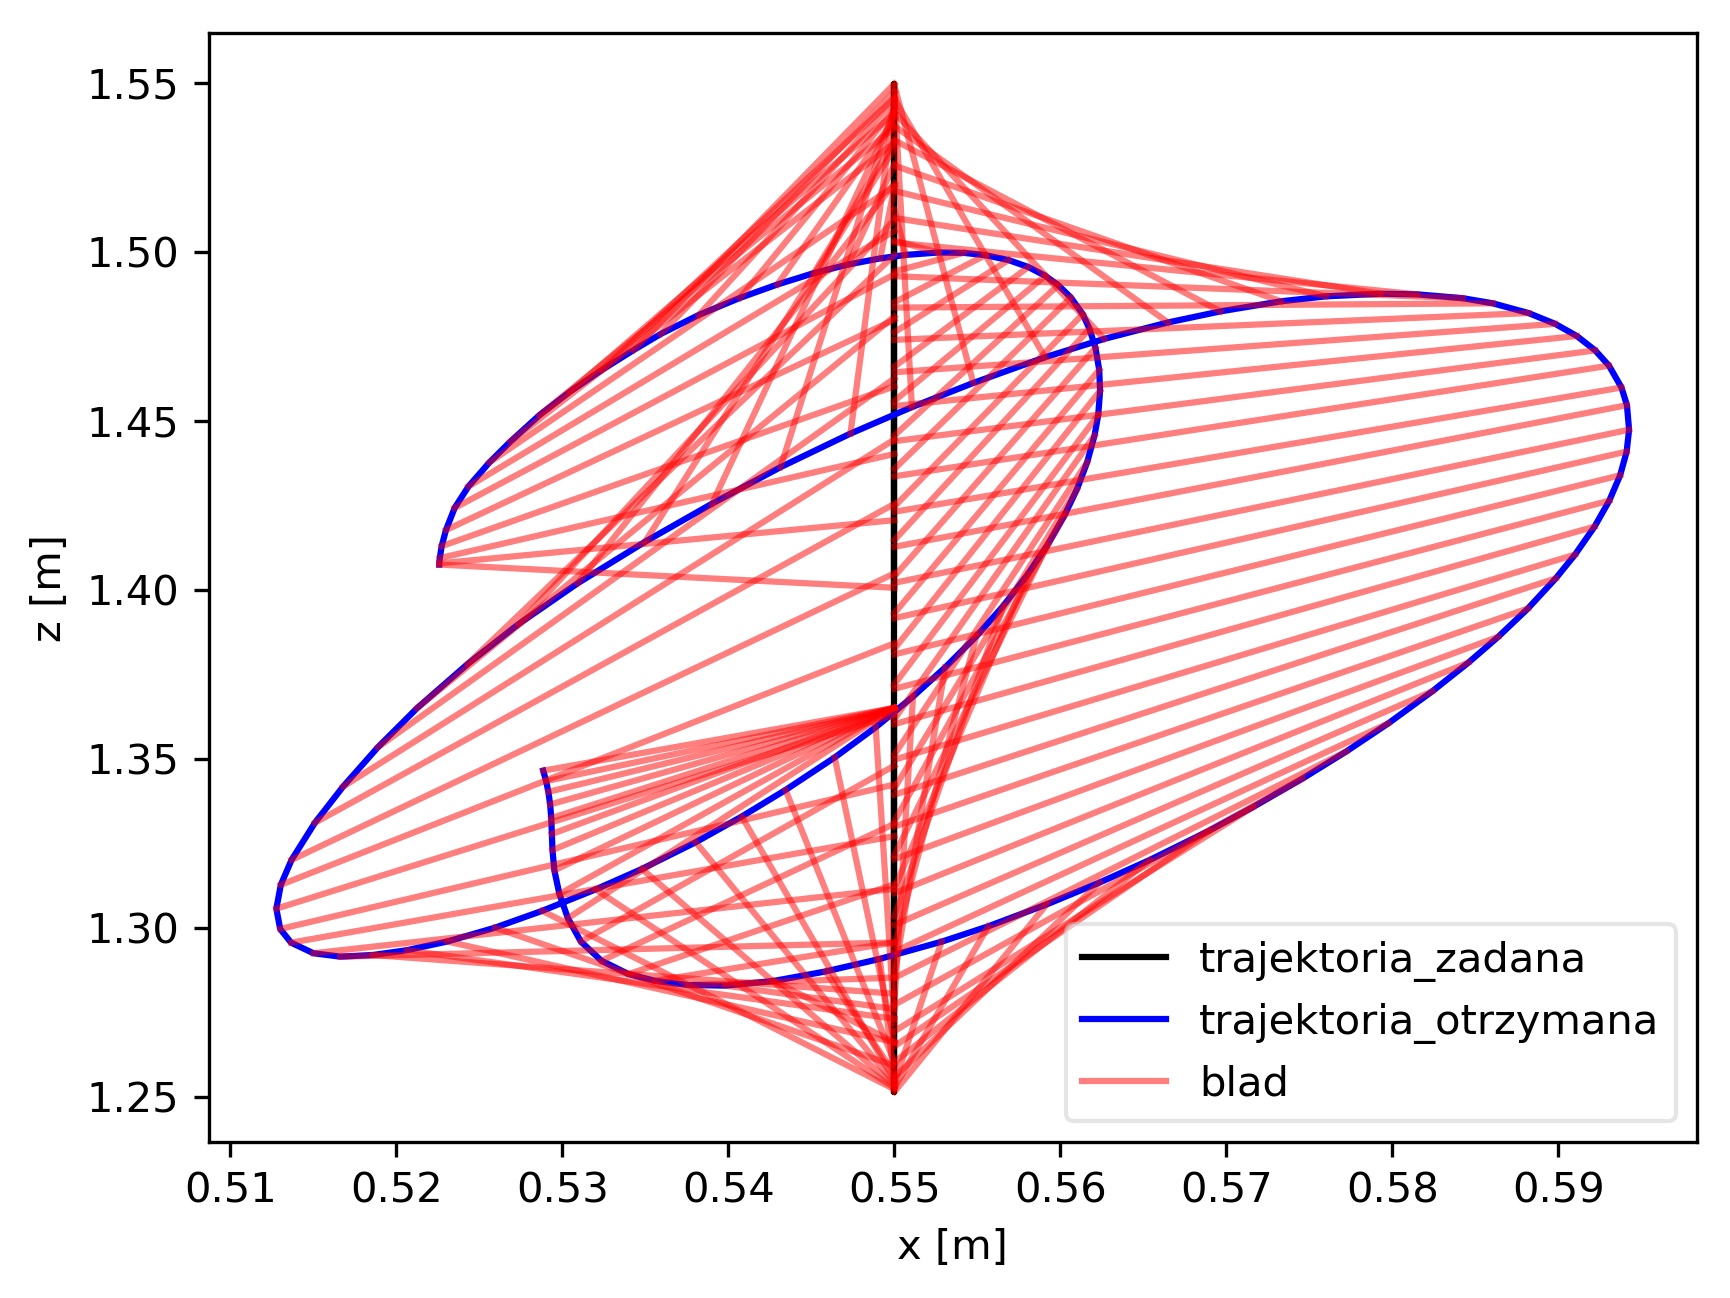
\includegraphics[width=.45\textwidth]{../../velma/przerobione_testy/out/osemka/xz_ate_plot_podnoszenie_miekki_bez_brak.png}
	}
	\hfill
	\subfigure[Zalaczony algorytm kompnesacji]{
		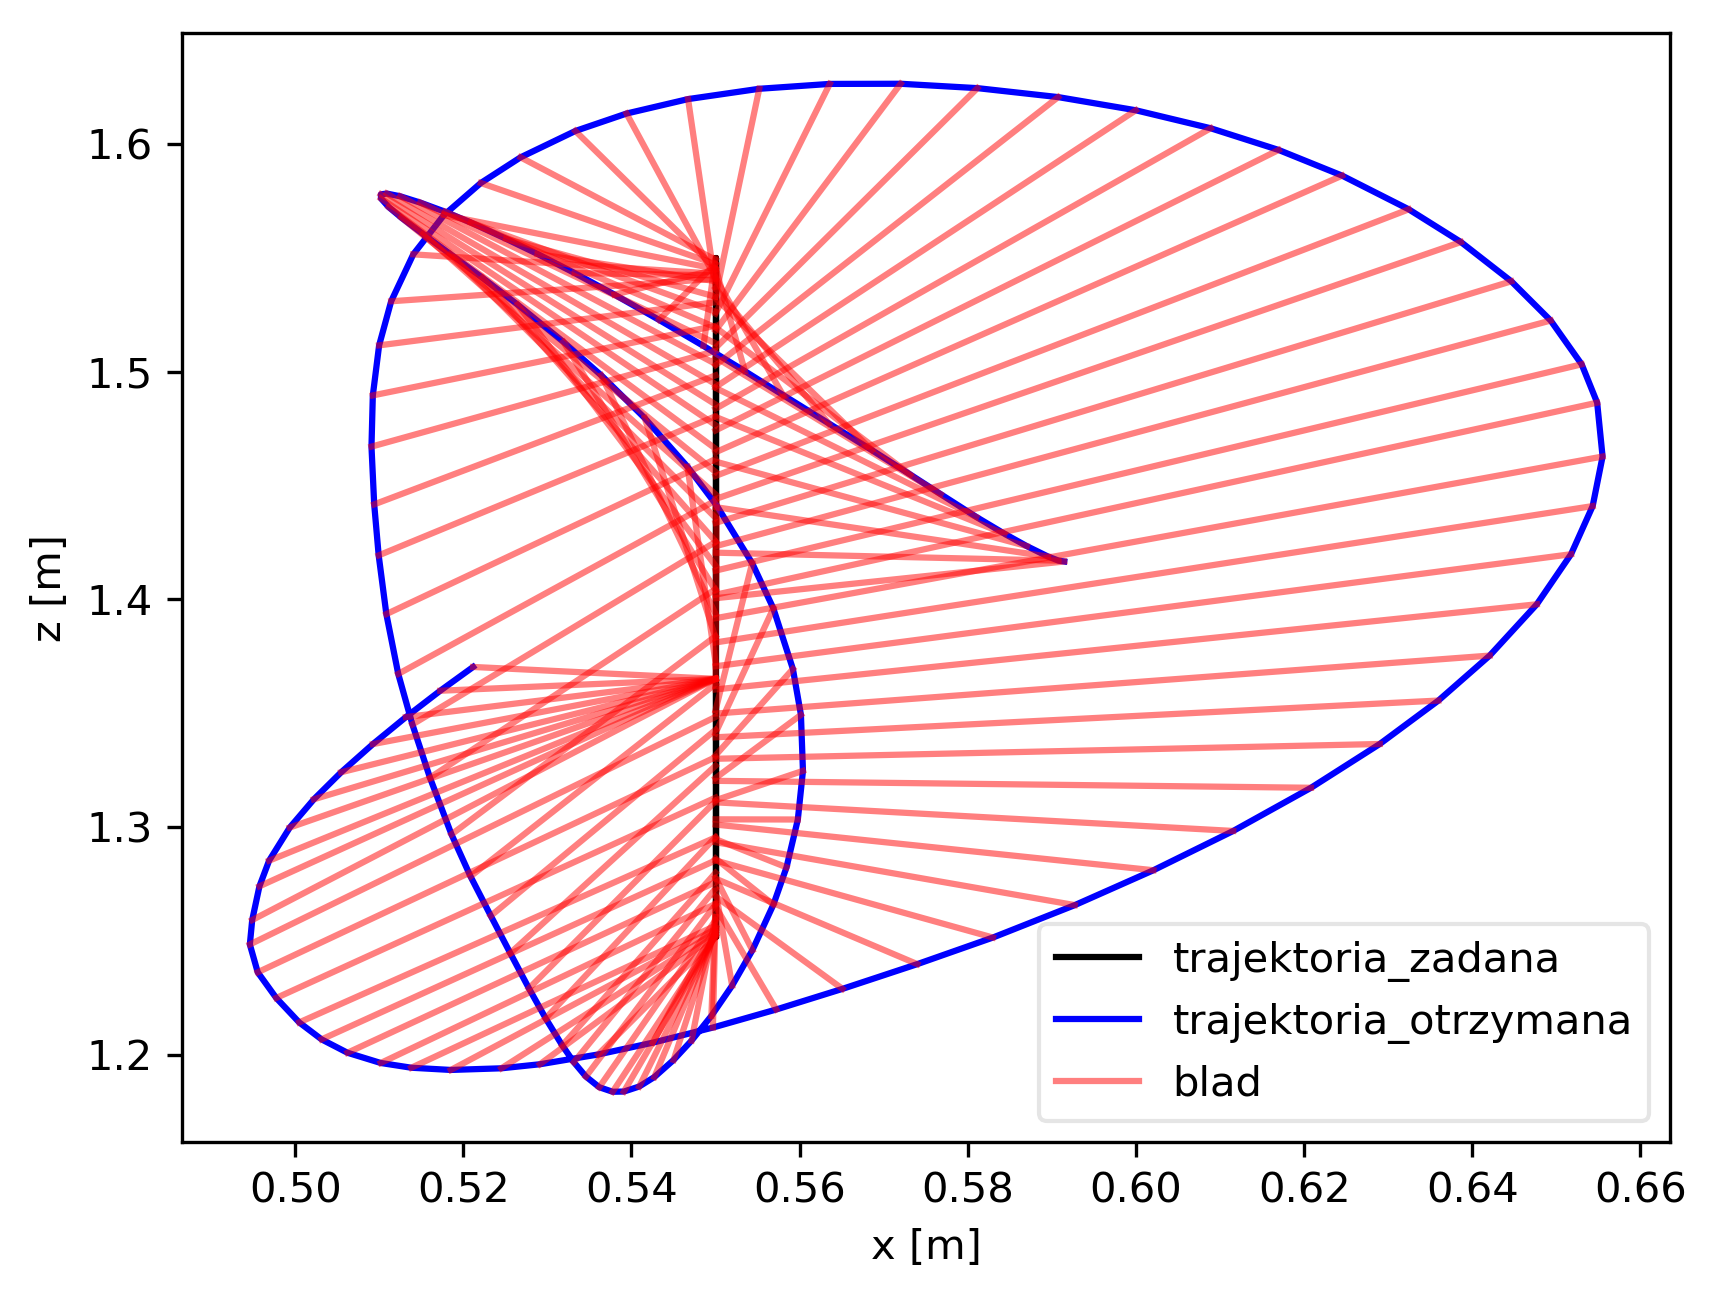
\includegraphics[width=.45\textwidth]{../../velma/przerobione_testy/out/osemka/xz_ate_plot_podnoszenie_miekki_komp_brak.png}
	}
	\caption{Ruch ósemkowy. Porównanie trajektorii chwytaka w~osiach $X$ i~$Z$}
	\label{fig:osemka_porow_komp_bok}
\end{figure}

\begin{figure}[H]
	\centering
	\subfigure[Trajektoria z~chwycona puszka]{
		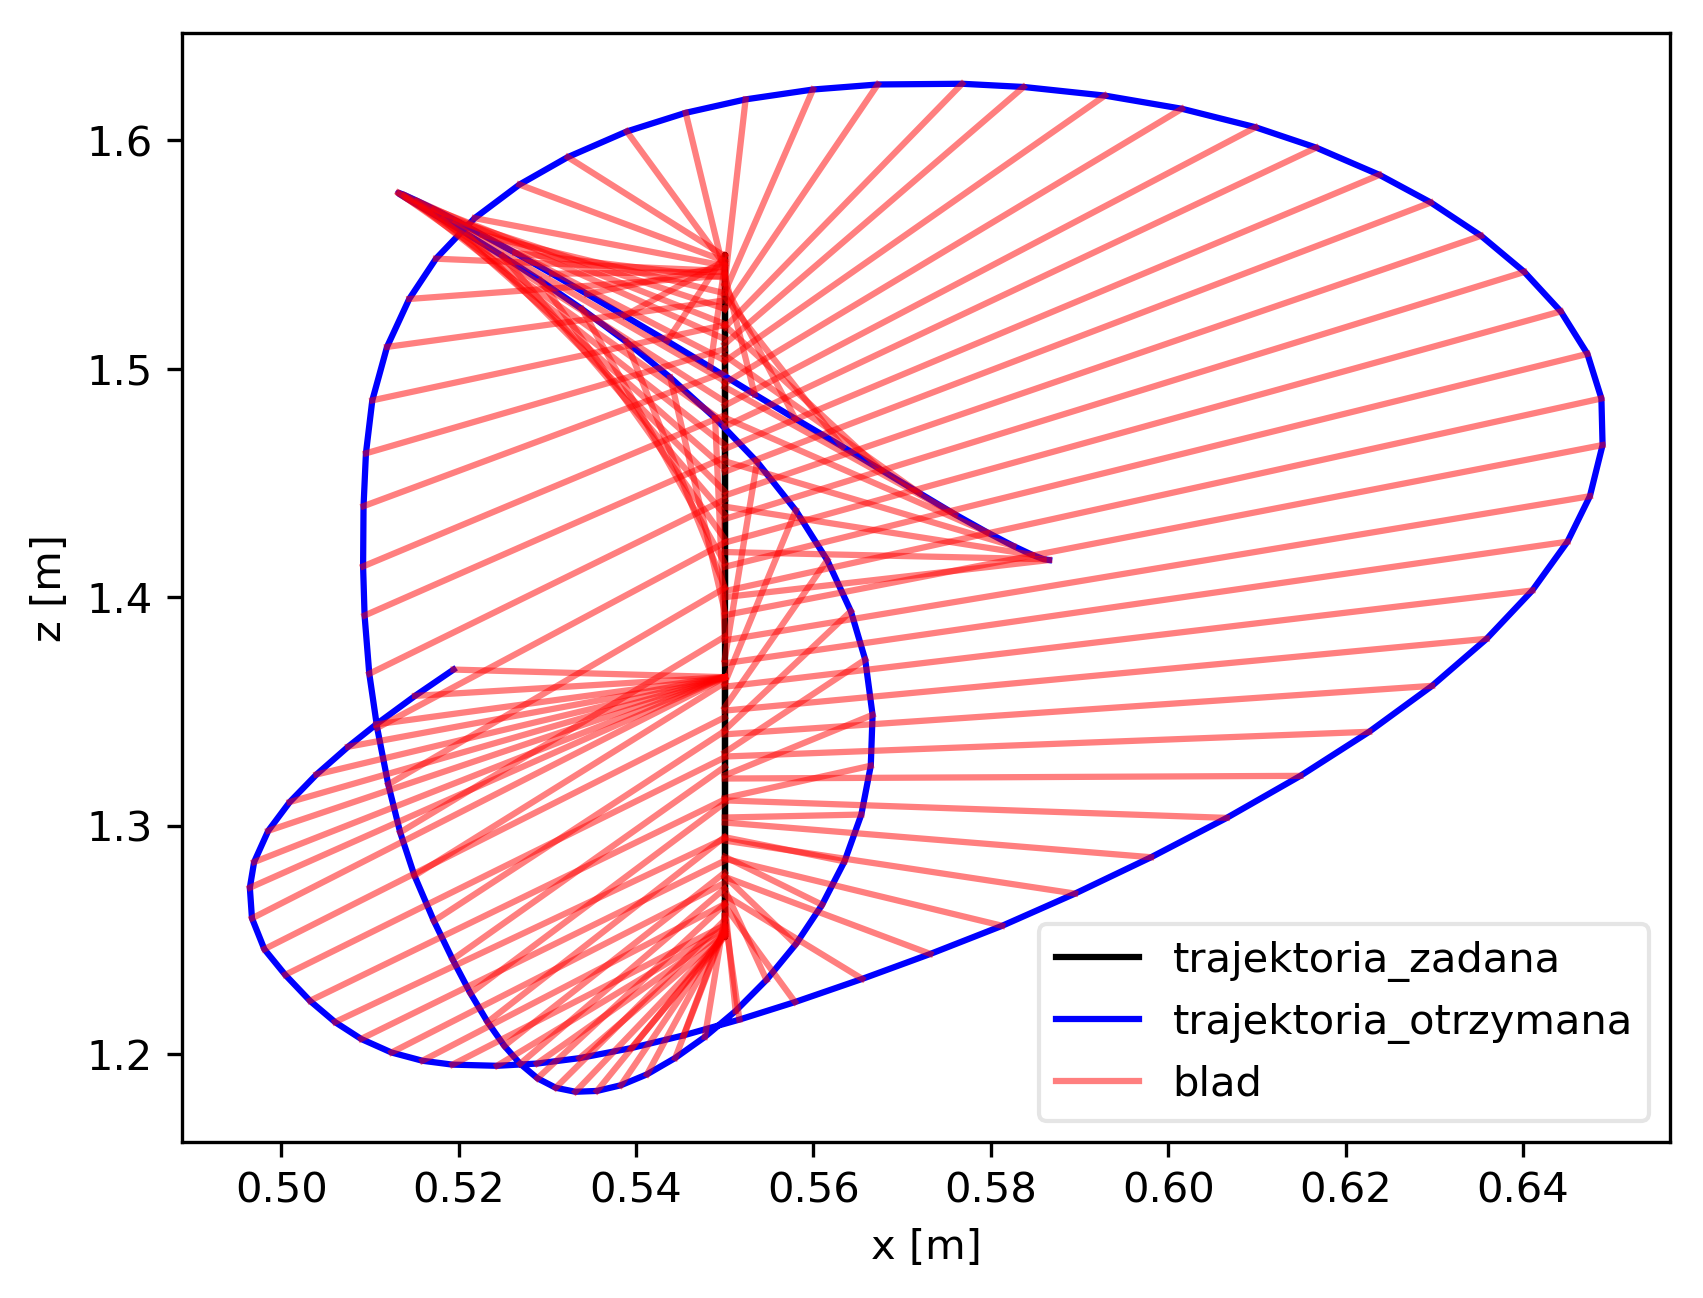
\includegraphics[width=.45\textwidth]{../../velma/przerobione_testy/out/osemka/xz_ate_plot_podnoszenie_miekki_komp_piwo.png}
	}
	\hfill
	\subfigure[Trajektoria z~chwycona wiertarka]{
		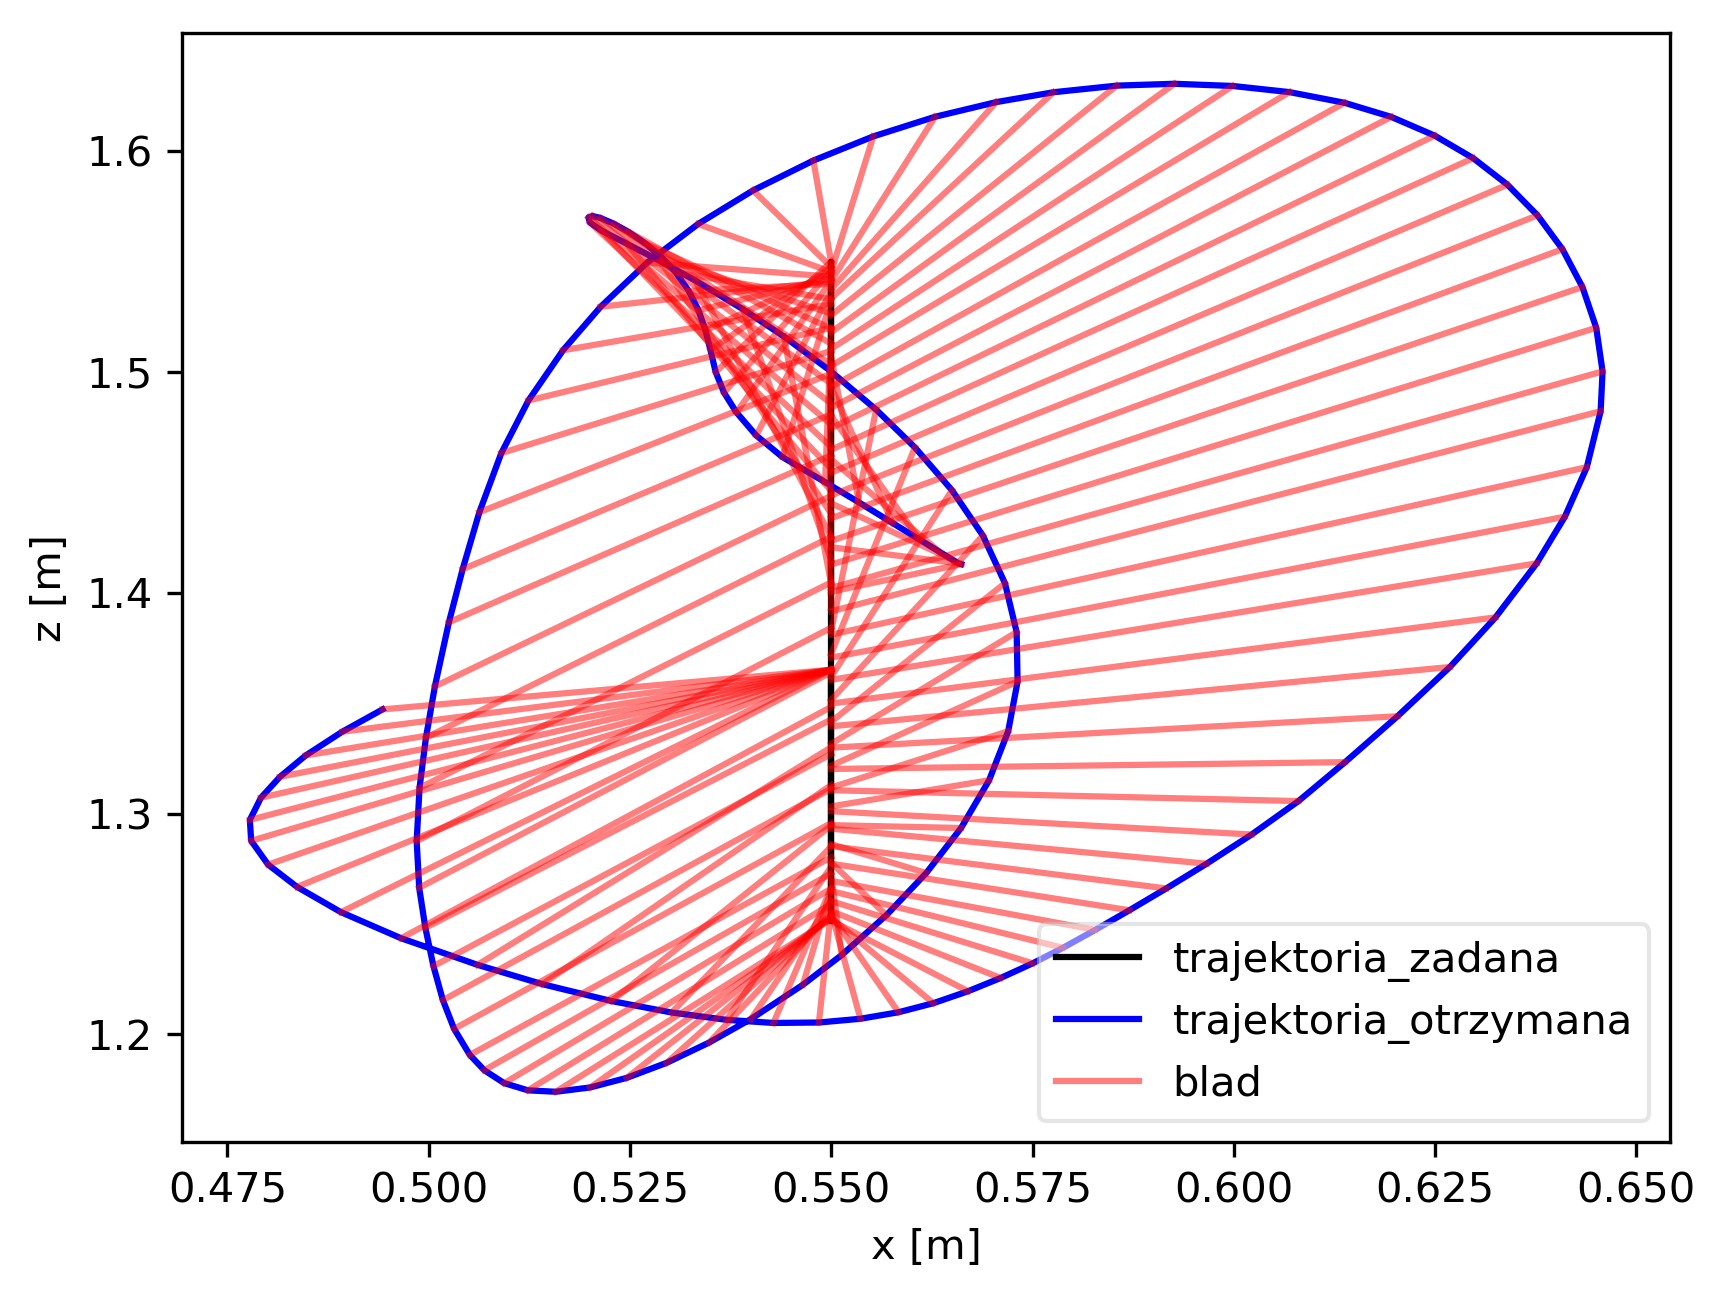
\includegraphics[width=.45\textwidth]{../../velma/przerobione_testy/out/osemka/xz_ate_plot_podnoszenie_miekki_komp_wiertarka.png}
	}
	\caption{Ruch ósemkowy. Porównanie trajektorii chwytaka w~osiach $X$ i~$Z$}
	\label{fig:osemka_porow_przedm_bok}
\end{figure}

% \begin{figure}[H]
% 	\centering
% 	\subfigure[Rzut na wprost]{
% 		\label{fig:osemka_porow_zbiorcze_a}
% 		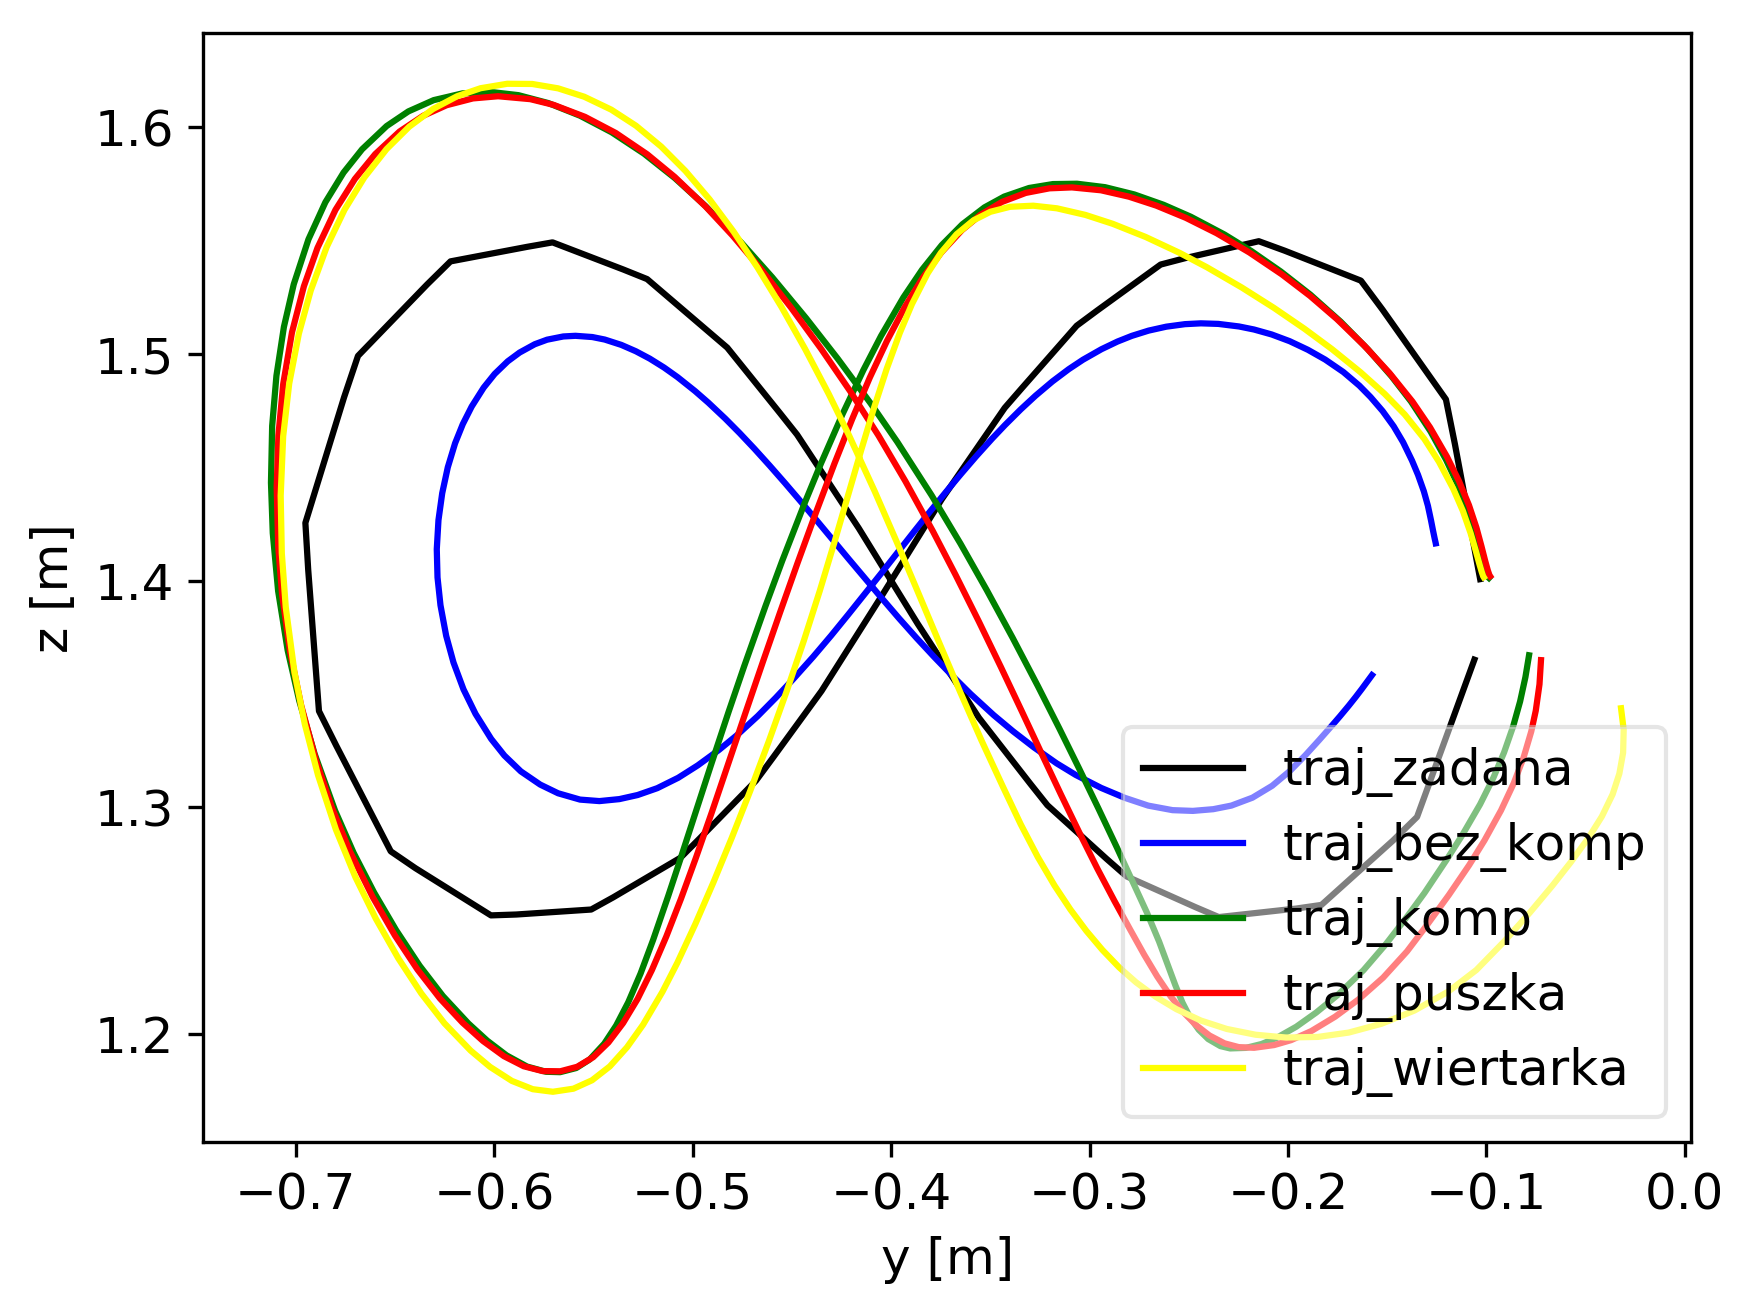
\includegraphics[width=.45\textwidth]{../../velma/przerobione_testy/out/osemka/common_yz.png}
% 	}
% 	\hfill
% 	\subfigure[Rzut z~boku]{
% 		\label{fig:osemka_porow_zbiorcze_b}
% 		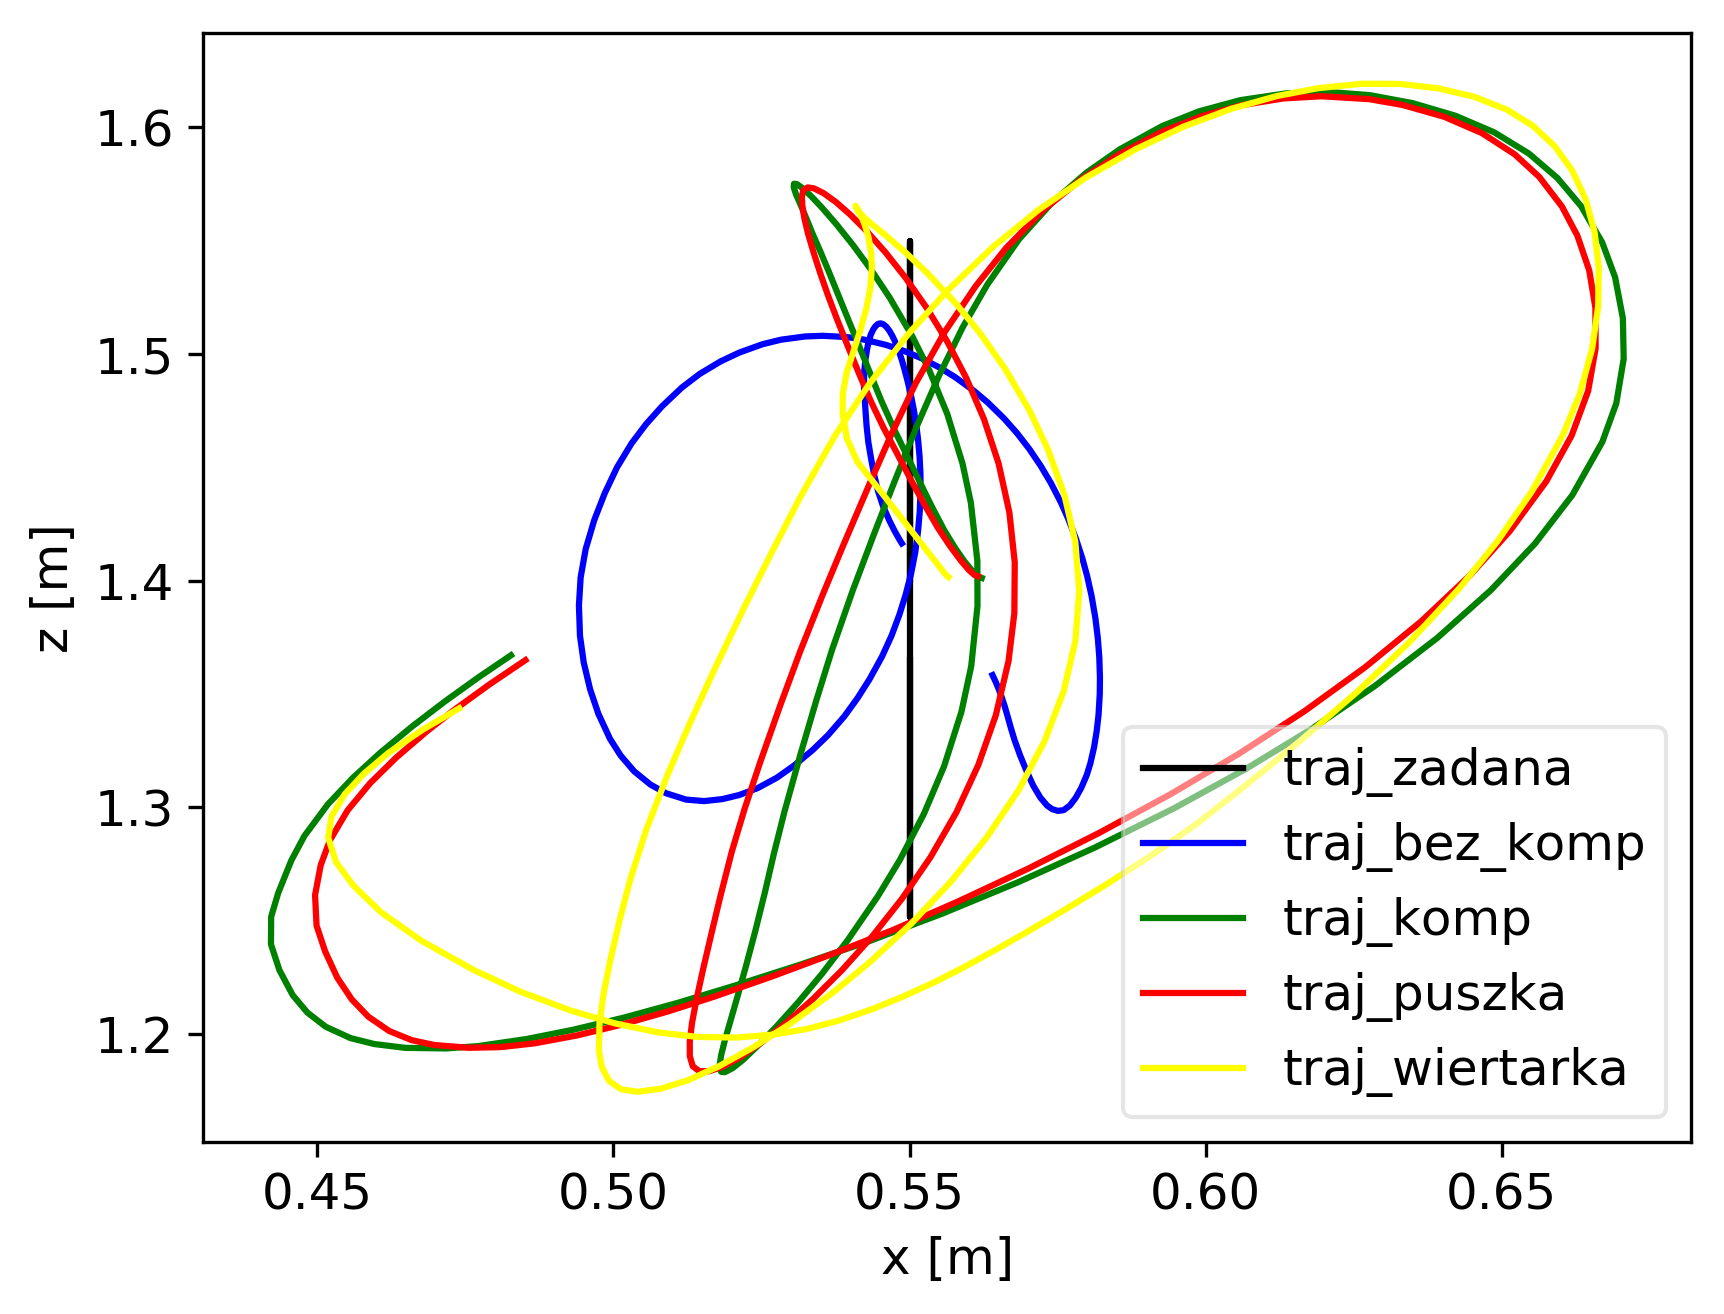
\includegraphics[width=.45\textwidth]{../../velma/przerobione_testy/out/osemka/common_xz.png}
% 	}
% 	\caption{Ruch ósemkowy. Porównanie wszystkich trajektorii bez zaznaczonego błędu}
% 	\label{fig:osemka_porow_zbiorcze}
% \end{figure}

\section{Ruch w~bok}

Eksperyment ma przetestować zachowanie algorytmu kompensacji przy ruchu końcówki w~bok. Trajektoria ruchu w~rzucie ATE została zaprezentowana na rys. \ref{fig:w_bok_miekki_porow_komp} i~\ref{fig:w_bok_miekki_porow_przedm}.
% Trajektoria widoczna z~boku (w osiach $X$ oraz $Z$) została zaprezentowana na rys. \ref{fig:w_bok_miekki_porow_komp_bok}, \ref{fig:w_bok_miekki_porow_przedm_bok} i~\ref{fig:w_bok_miekki_porow_zbiorcze_b}.
\begin{figure}[H]
	\centering
	\subfigure[Oś $X$]{
		\label{fig:w_bok_miekki_ax}
		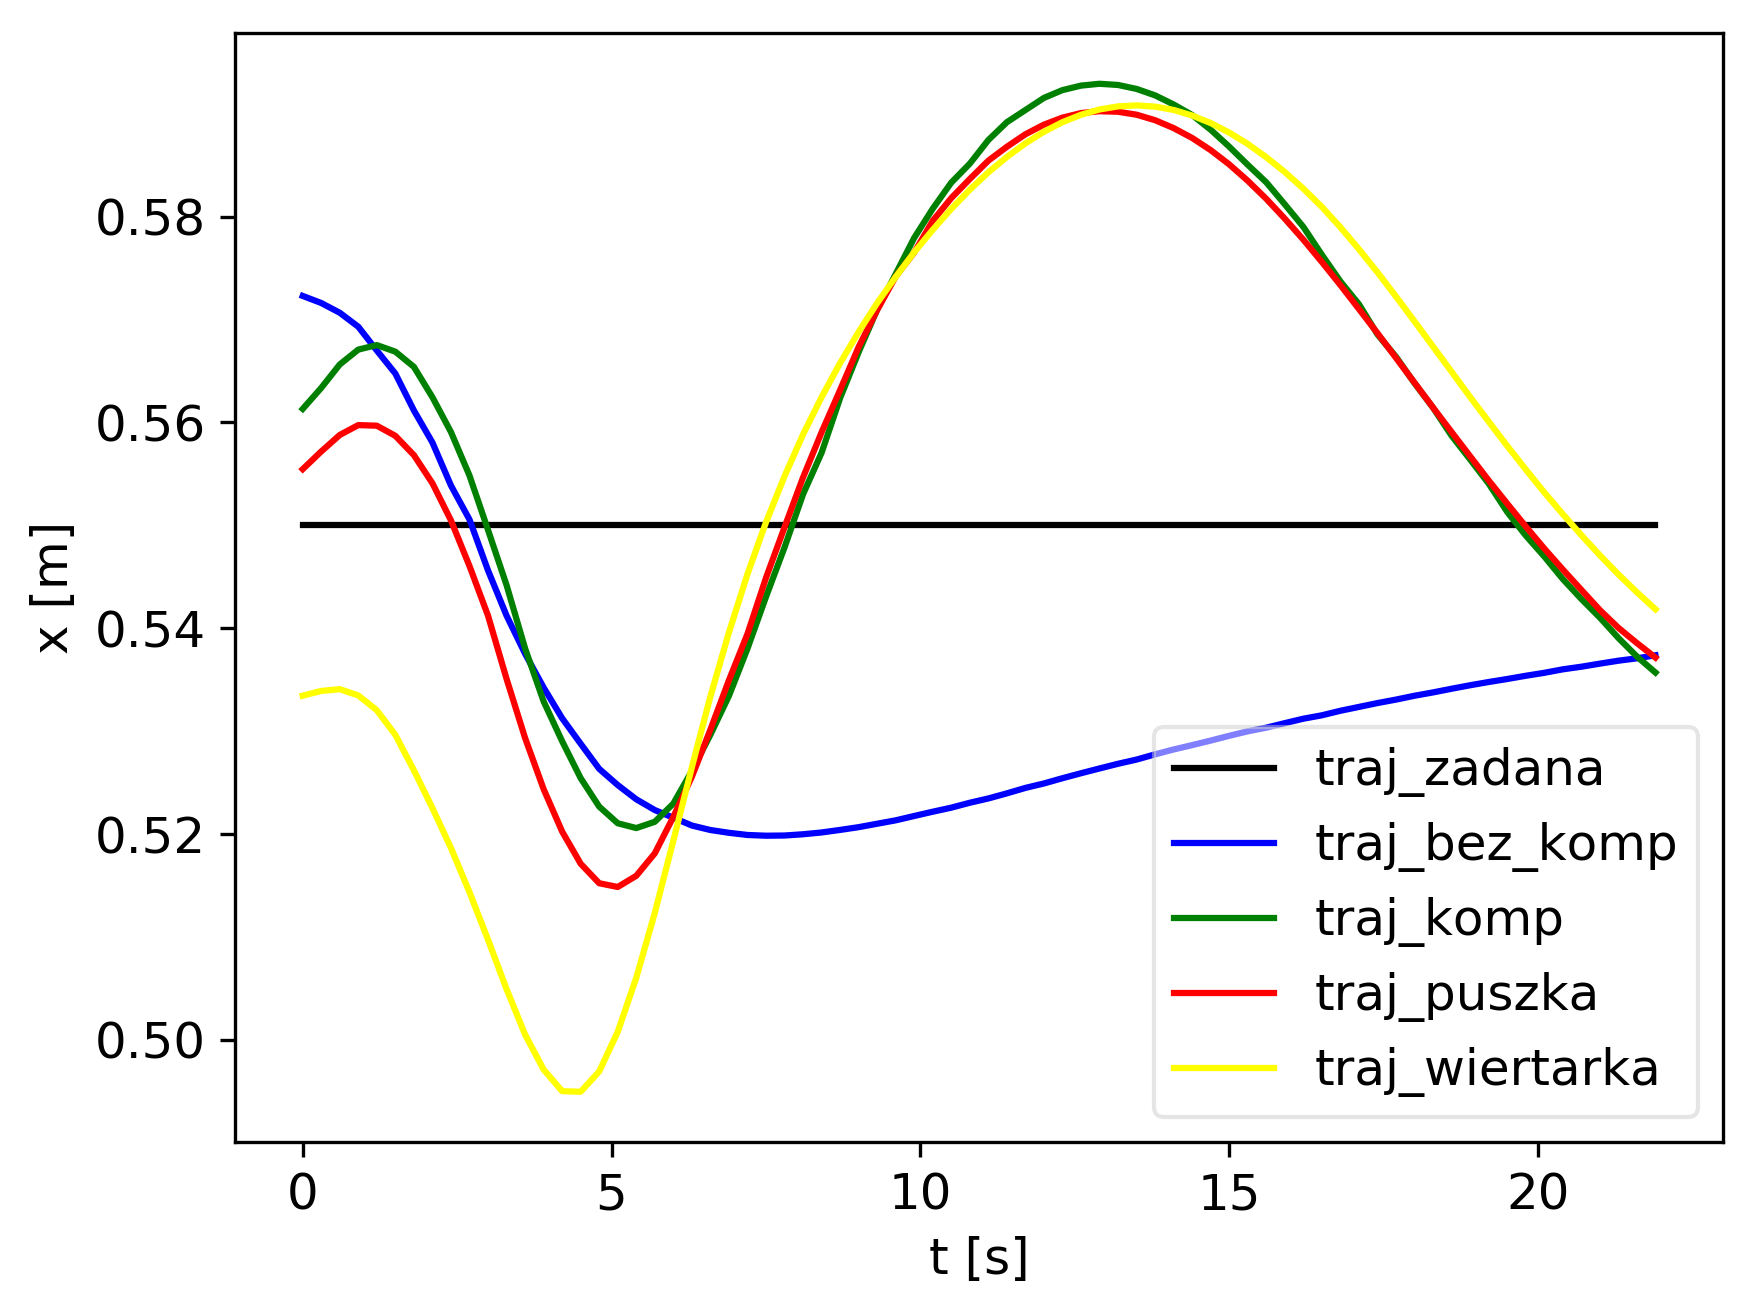
\includegraphics[width=.45\textwidth]{../../velma/przerobione_testy/out/w_bok_miekki/common_ax.png}
	}
	\hfill
	\subfigure[Oś $Y$]{
		\label{fig:w_bok_miekki_ay}
		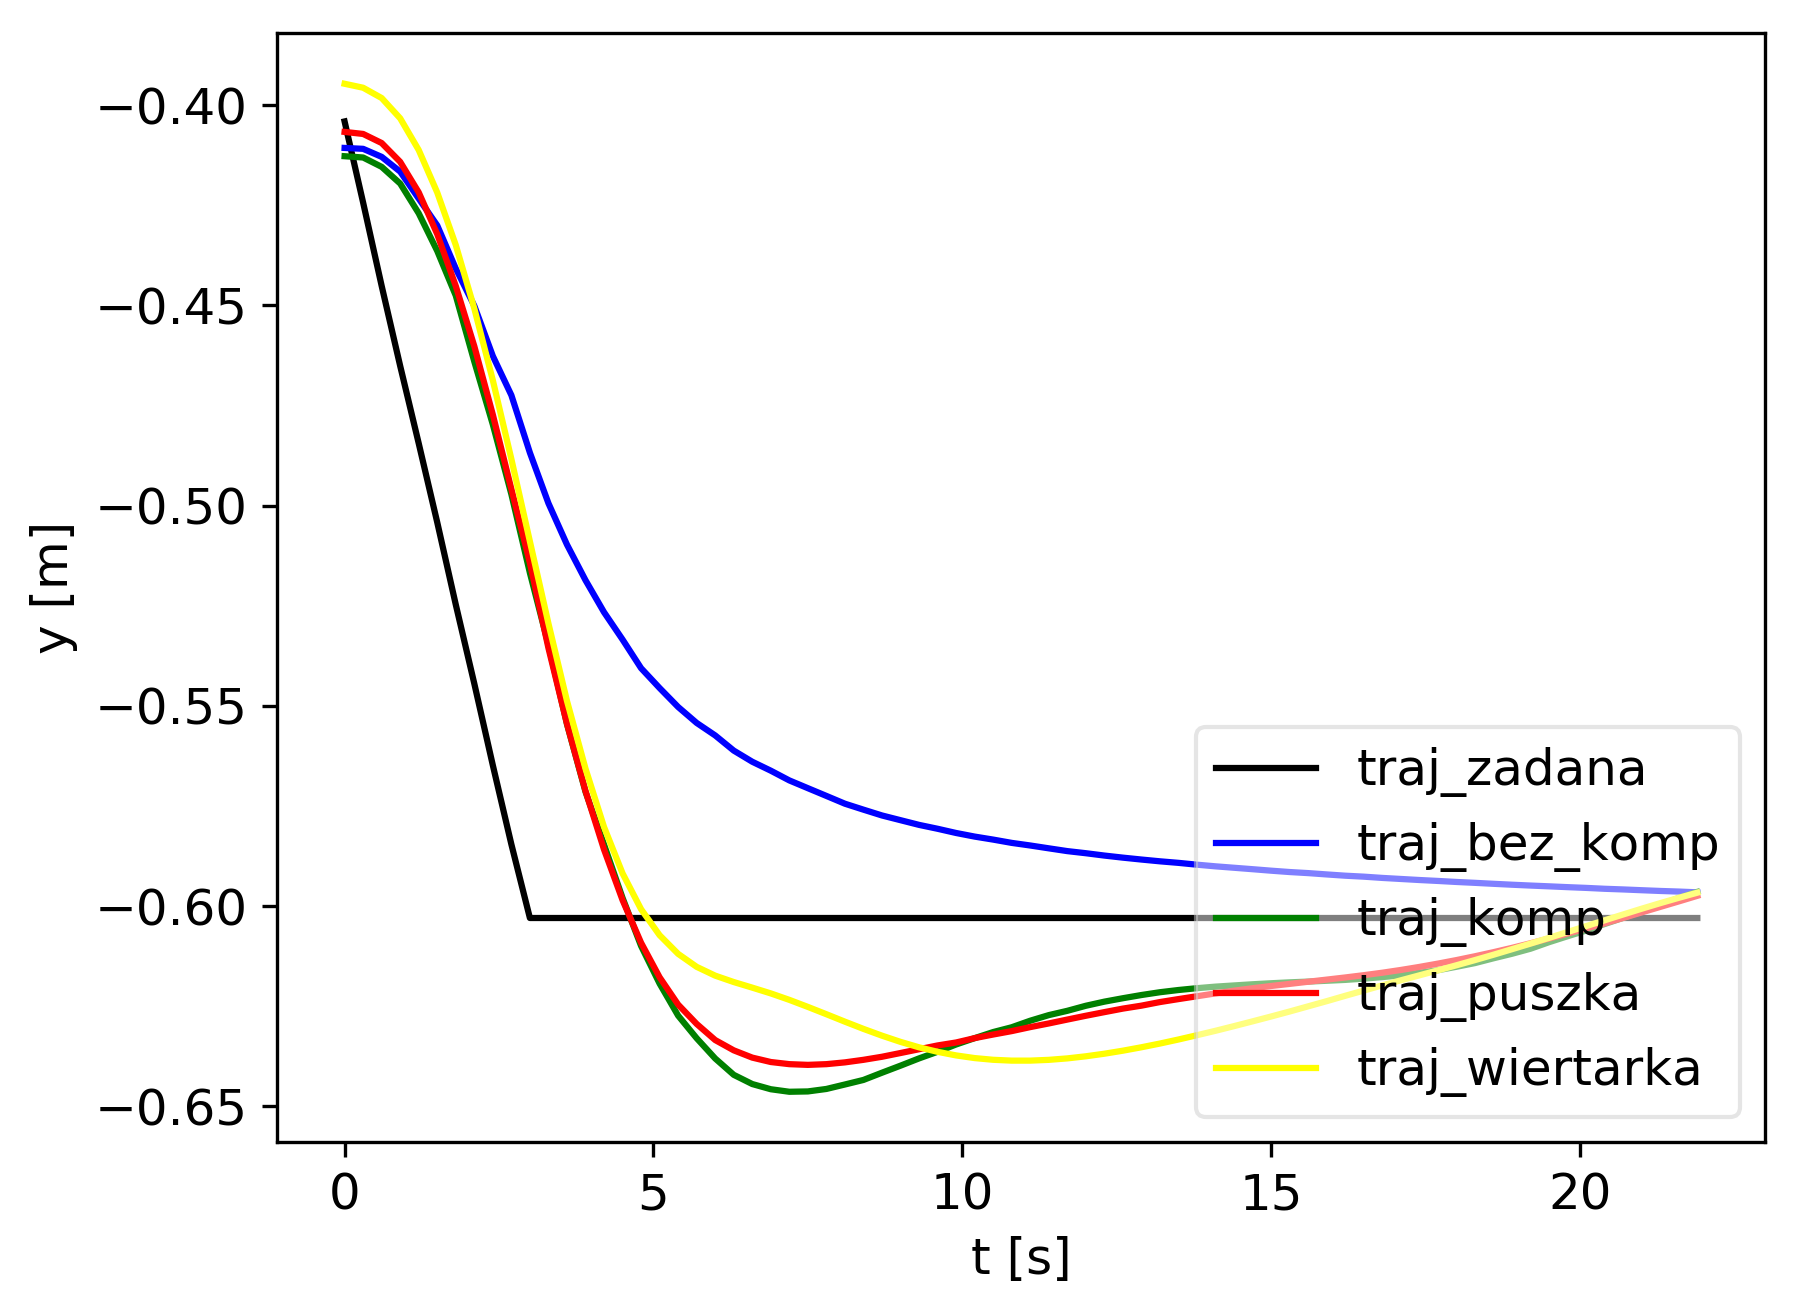
\includegraphics[width=.45\textwidth]{../../velma/przerobione_testy/out/w_bok_miekki/common_ay.png}
	}
	
	\hfill
	\subfigure[Oś $Z$]{
		\label{fig:w_bok_miekki_az}
		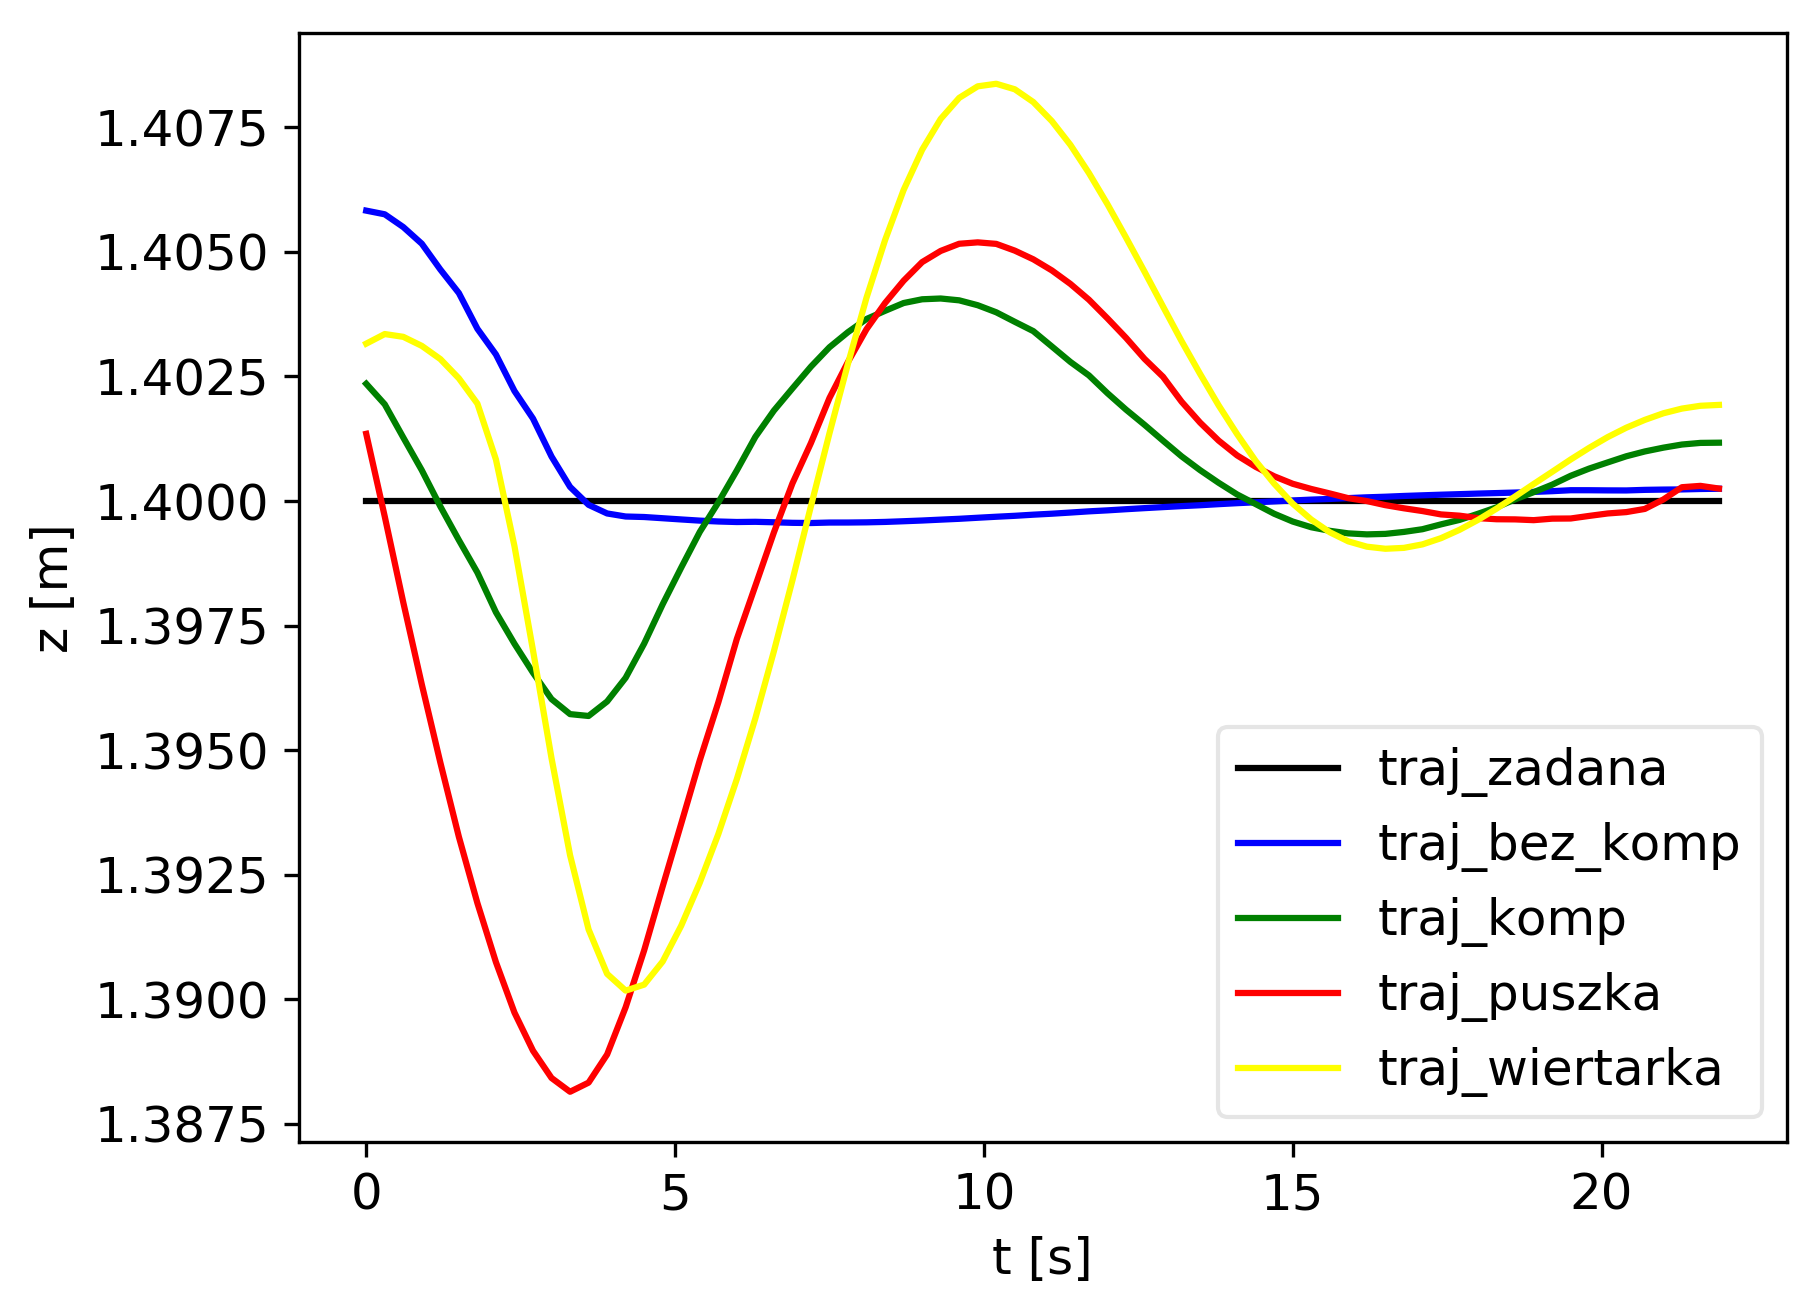
\includegraphics[width=.45\textwidth]{../../velma/przerobione_testy/out/w_bok_miekki/common_az.png}
	}

	\caption{Ruch w~bok. Porównanie trajektorii pozycji w~zależności od czasu.}
	\label{fig:w_bok_miekki_a}

\end{figure}

\begin{figure}[H]
	\centering
	\subfigure[Brak algorytmu kompensacji]{
		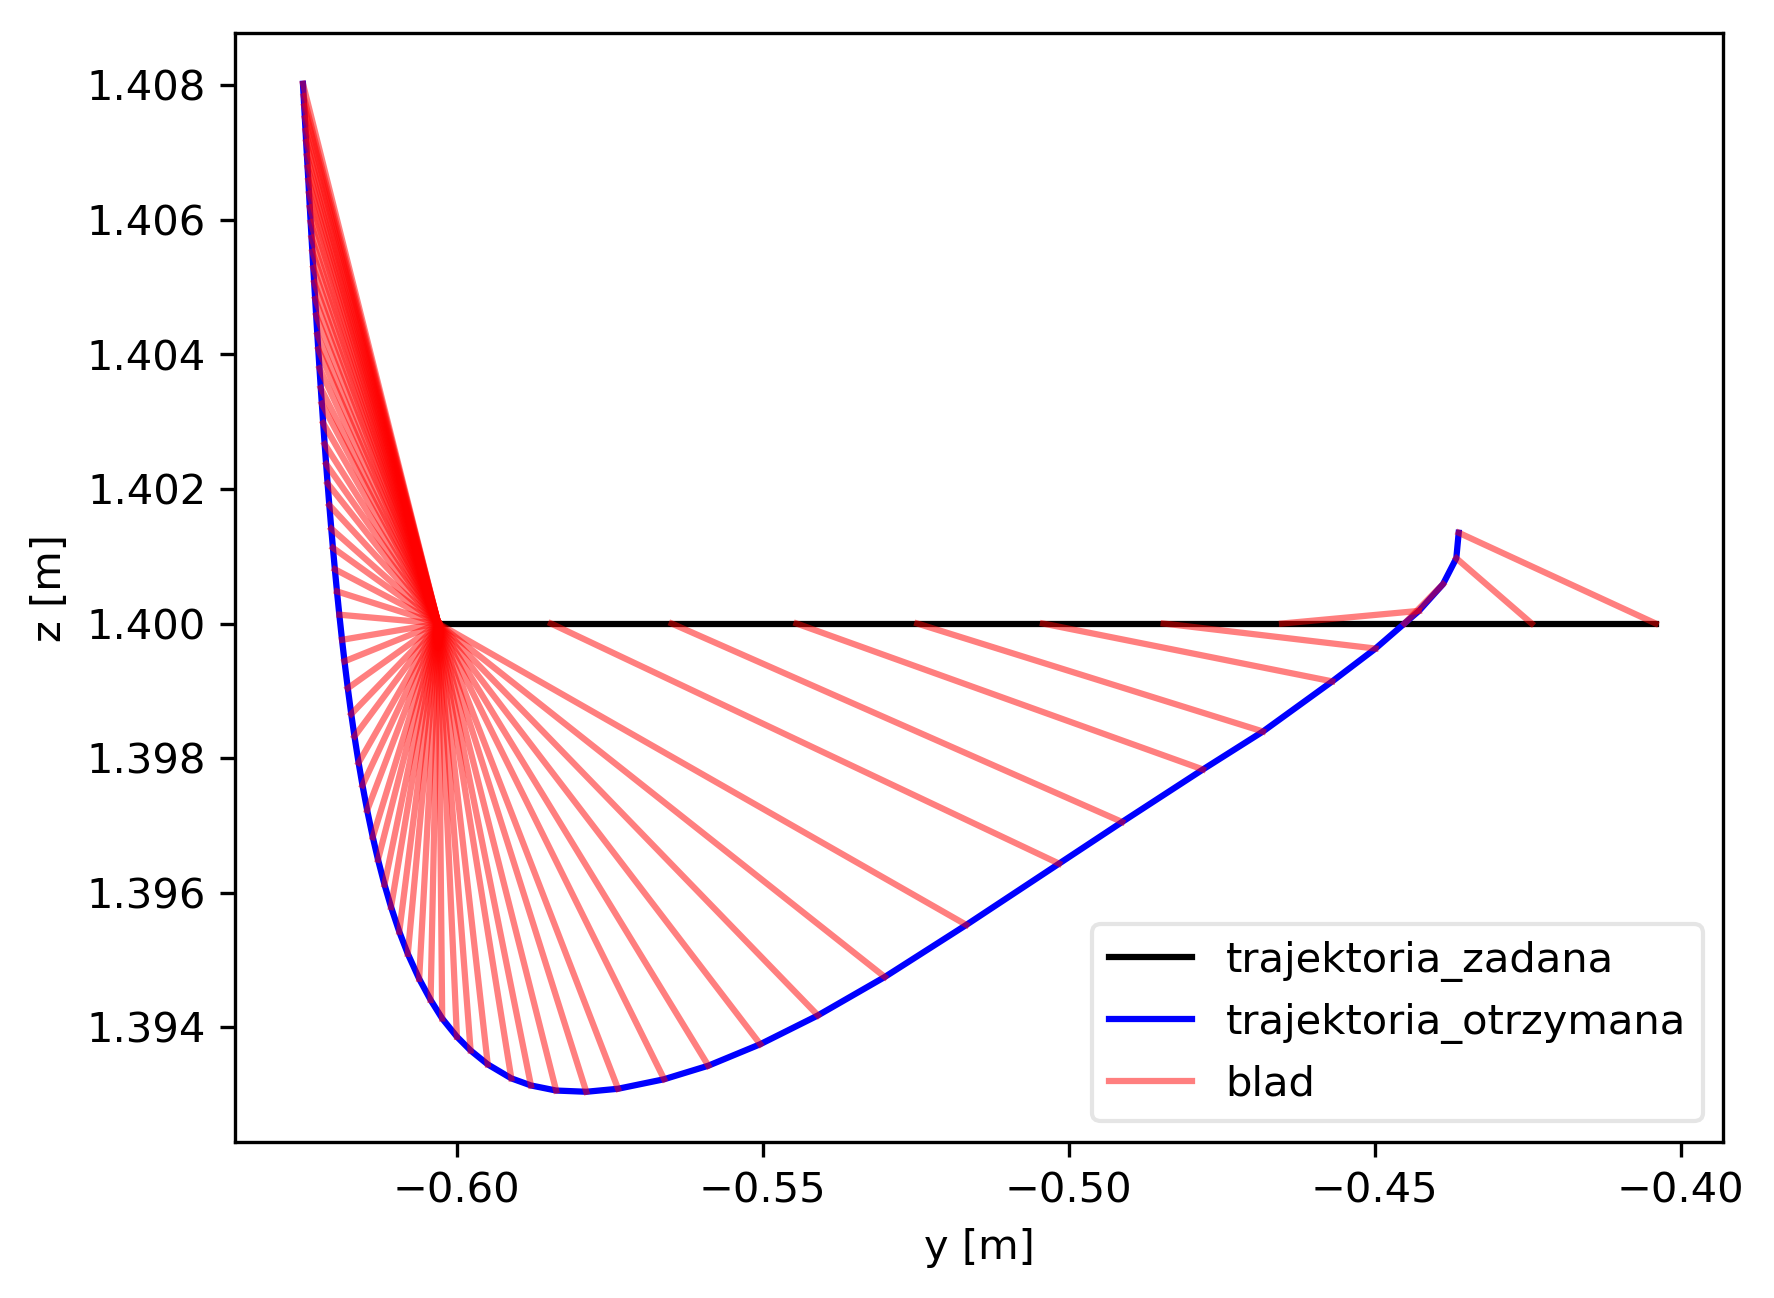
\includegraphics[width=.45\textwidth]{../../velma/przerobione_testy/out/w_bok_miekki/yz_ate_plot_podnoszenie_miekki_bez_brak.png}
	}
	\hfill
	\subfigure[Zalaczony algorytm kompnesacji]{
		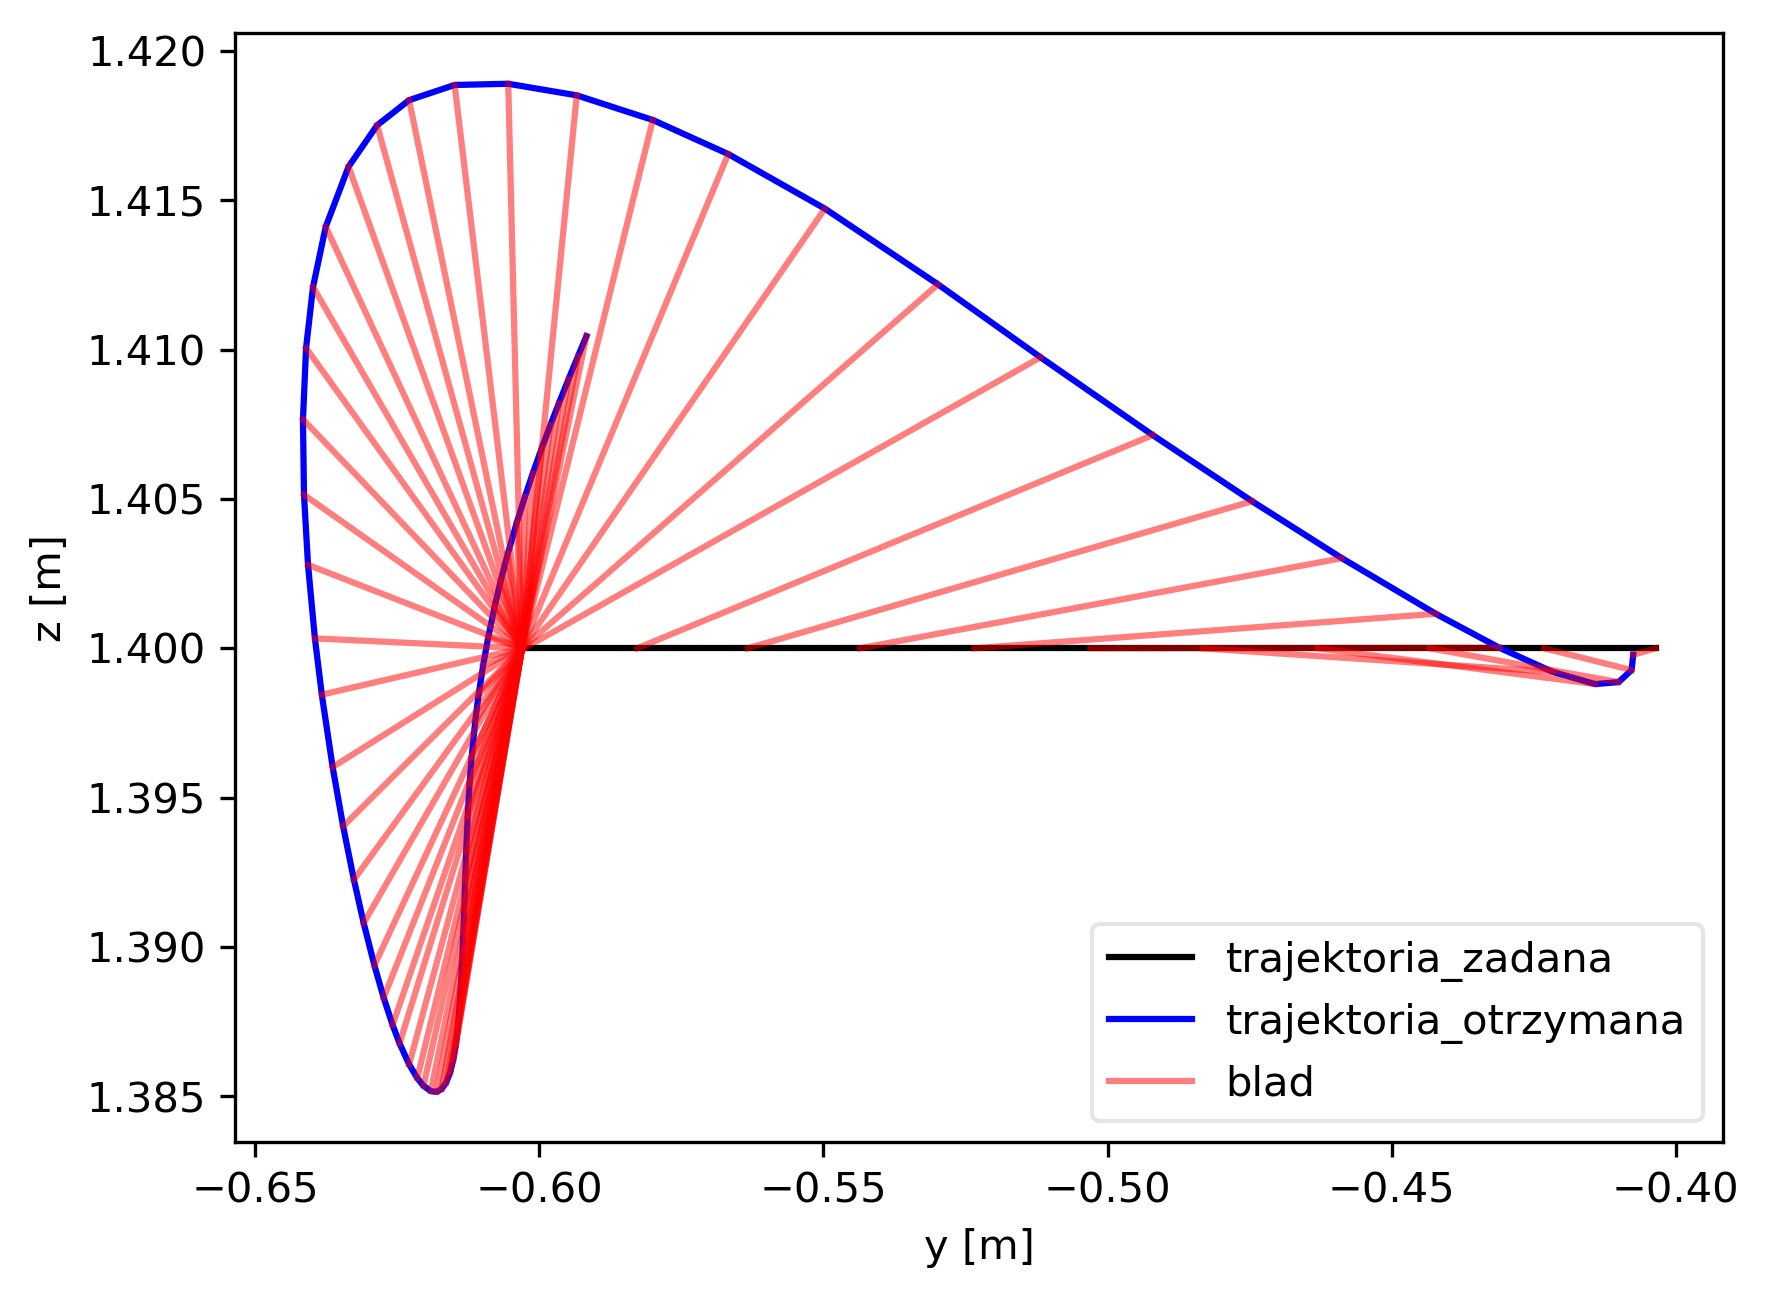
\includegraphics[width=.45\textwidth]{../../velma/przerobione_testy/out/w_bok_miekki/yz_ate_plot_podnoszenie_miekki_komp_brak.png}
	}
	\caption{Ruch w~bok. Porównanie trajektorii chwytaka w~osiach $Y$ i~$Z$}
	\label{fig:w_bok_miekki_porow_komp}
\end{figure}


\begin{figure}[H]
	\centering
	\subfigure[Kąt osi $X$]{
		\label{fig:w_bok_miekki_rotx}
		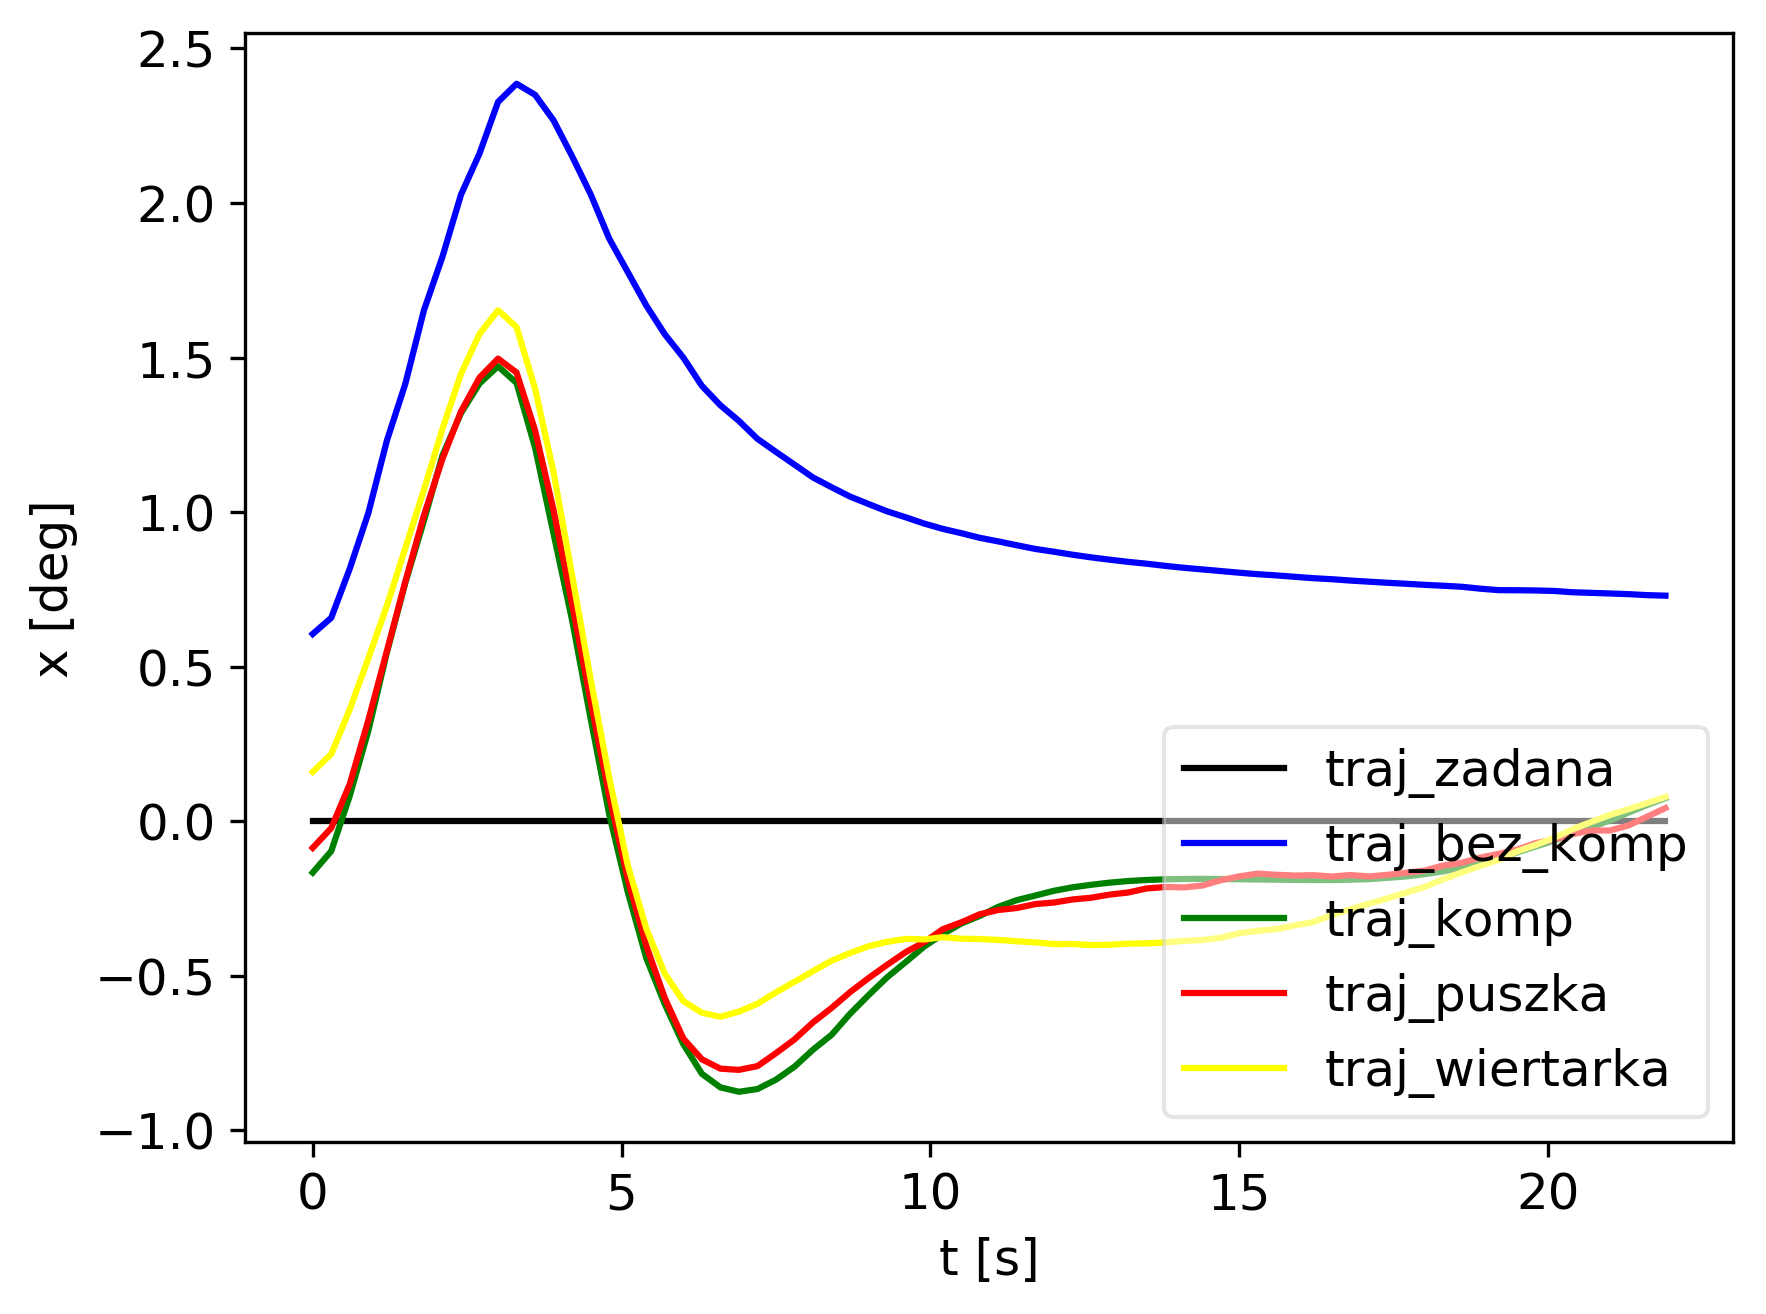
\includegraphics[width=.45\textwidth]{../../velma/przerobione_testy/out/w_bok_miekki/common_rotx.png}
	}
	\hfill
	\subfigure[Kąt osi $Y$]{
		\label{fig:w_bok_miekki_roty}
		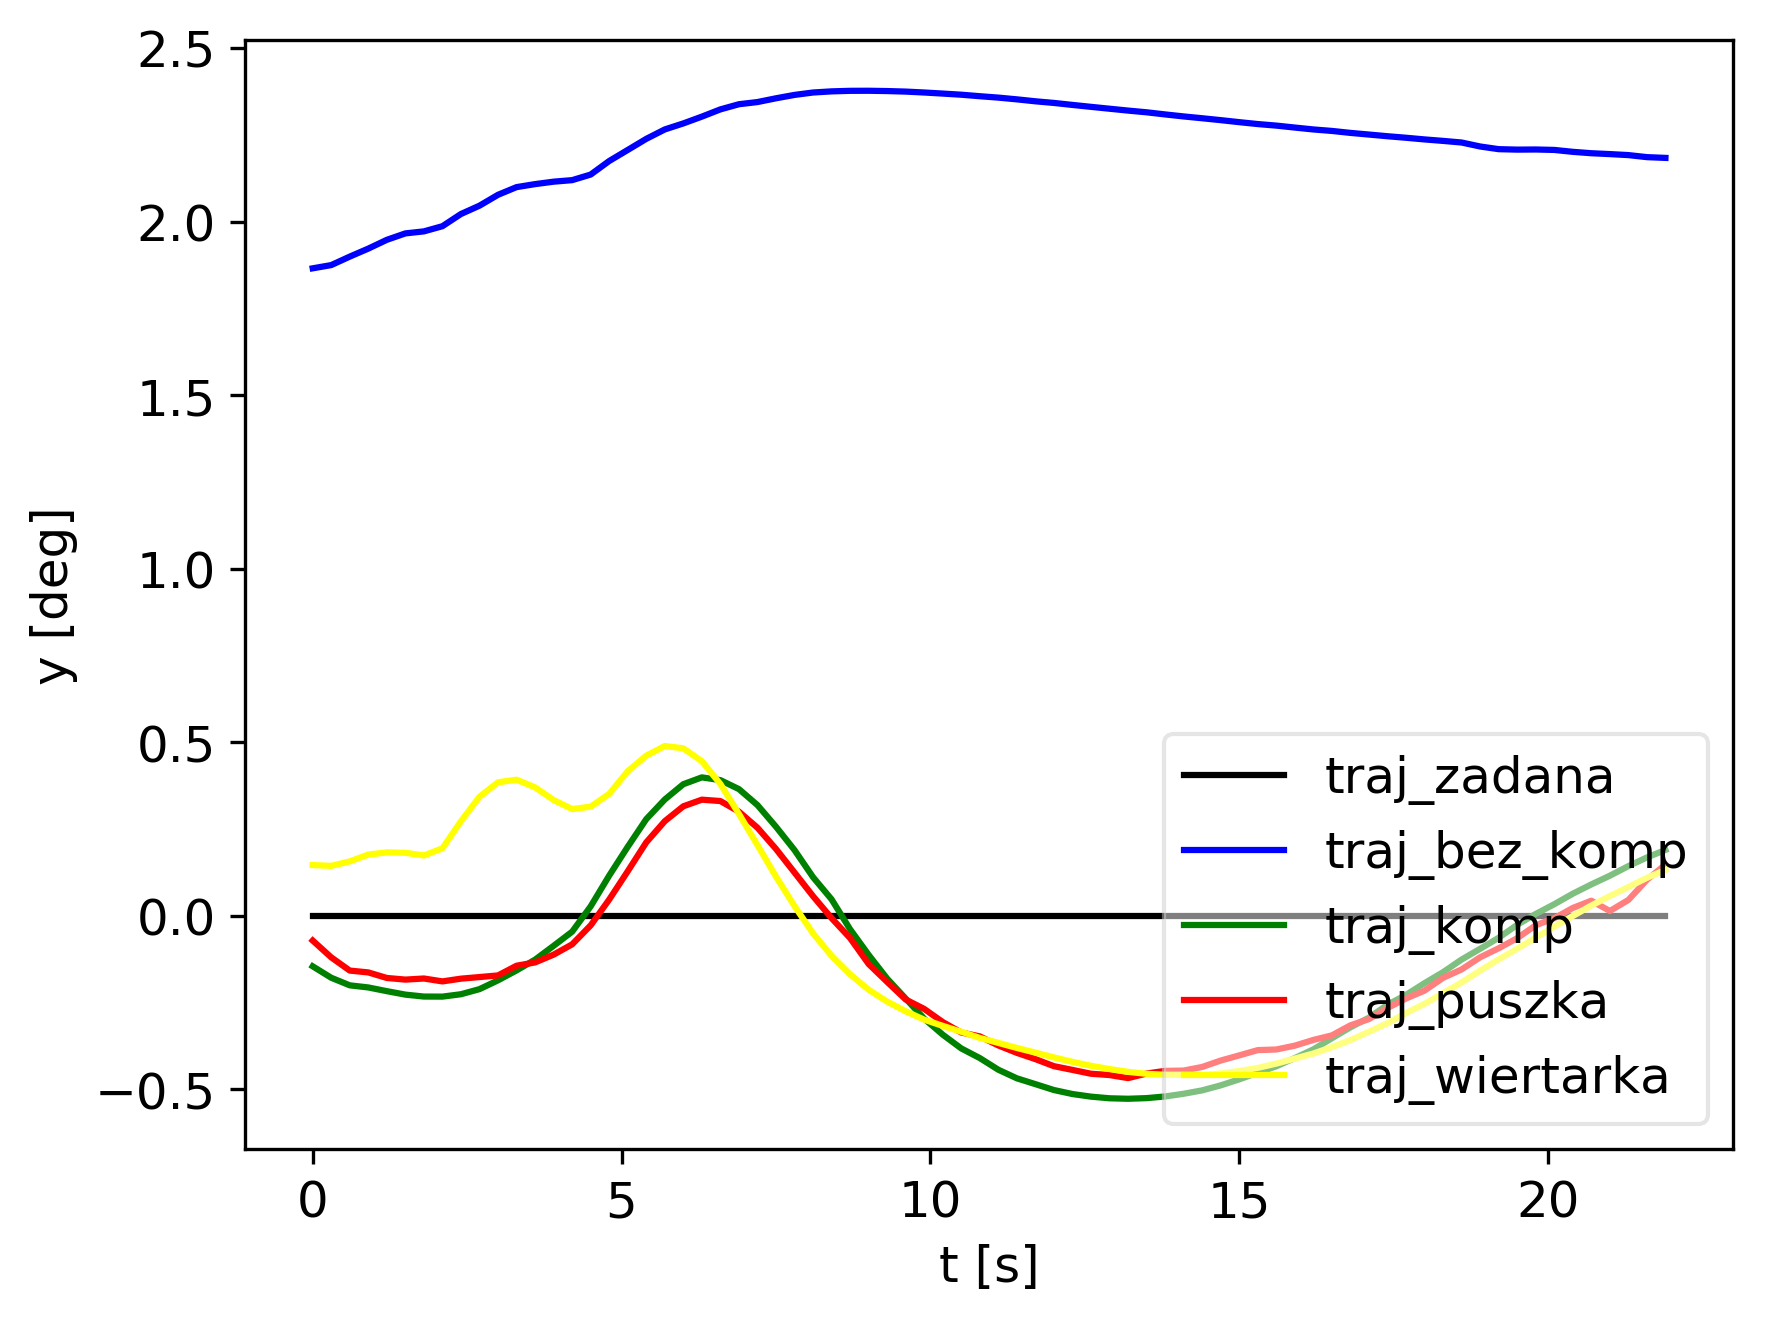
\includegraphics[width=.45\textwidth]{../../velma/przerobione_testy/out/w_bok_miekki/common_roty.png}
	}
	
	\subfigure[Kąt osi $Z$]{
		\label{fig:w_bok_miekki_rotz}
		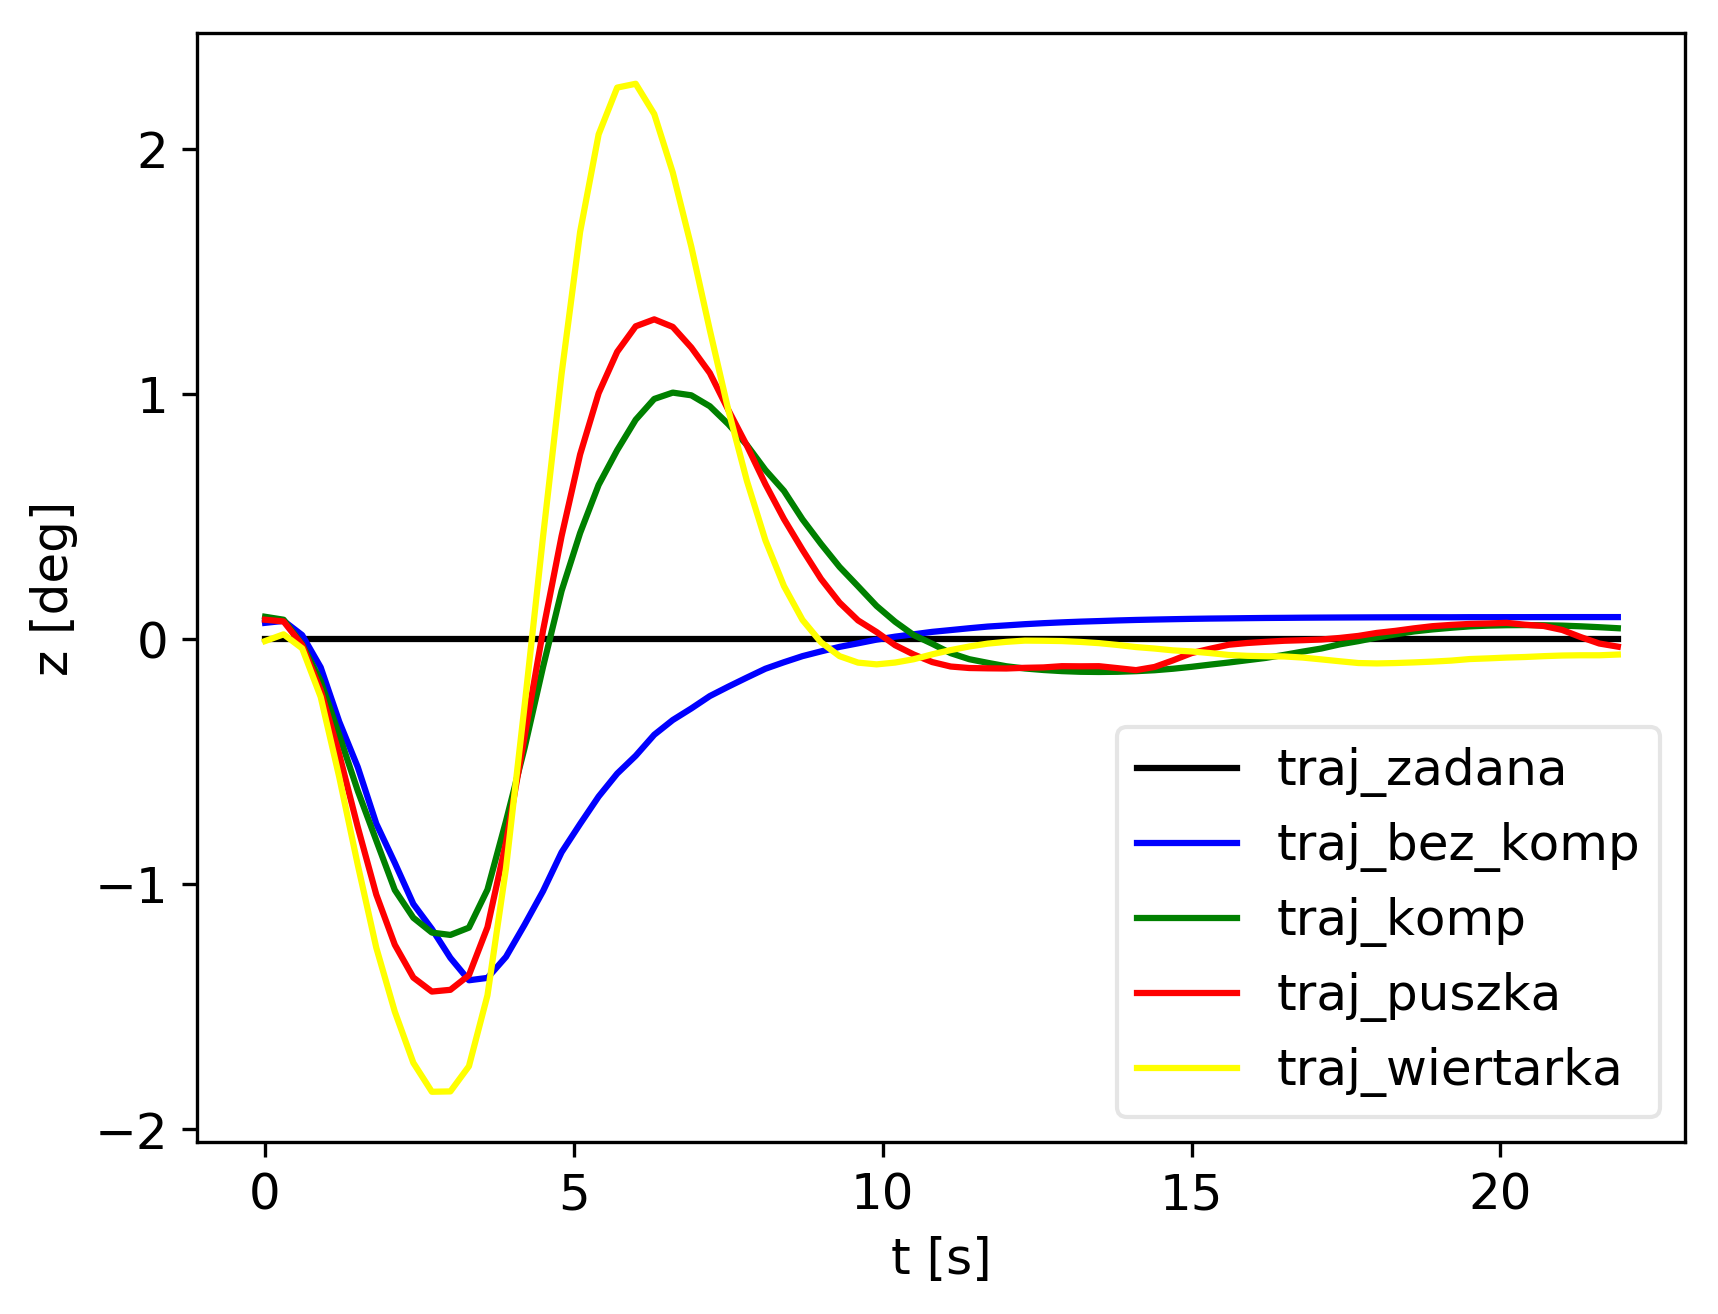
\includegraphics[width=.45\textwidth]{../../velma/przerobione_testy/out/w_bok_miekki/common_rotz.png}
	}

	\caption{Ruch w~bok. Porównanie trajektorii kątów w~notacji Eulera w~zależności od czasu.}
	\label{fig:w_bok_miekki_rot}

\end{figure}



\begin{figure}[H]
	\centering
	\subfigure[Trajektoria z~chwycona puszka]{
		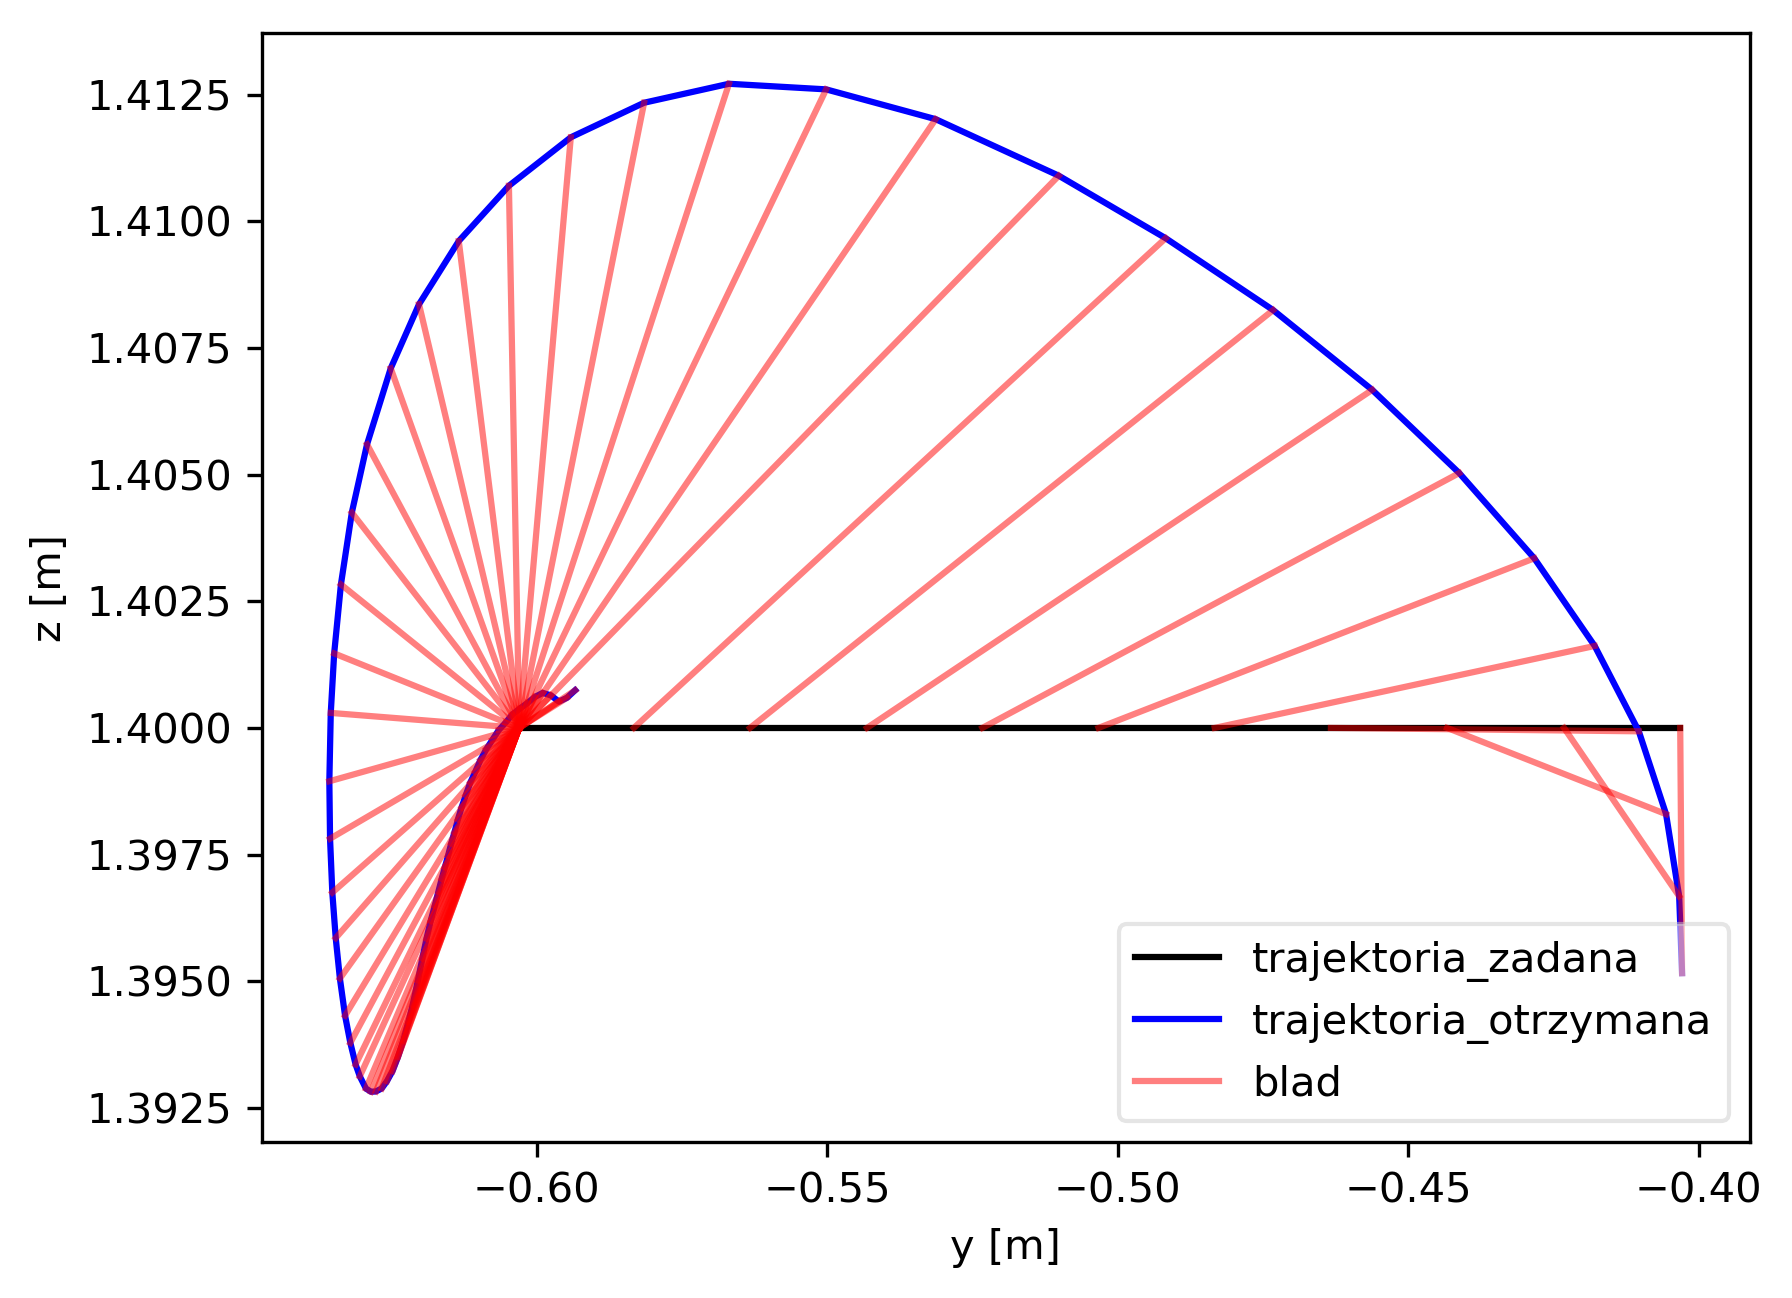
\includegraphics[width=.45\textwidth]{../../velma/przerobione_testy/out/w_bok_miekki/yz_ate_plot_podnoszenie_miekki_komp_piwo.png}
	}
	\hfill
	\subfigure[Trajektoria z~chwycona wiertarka]{
		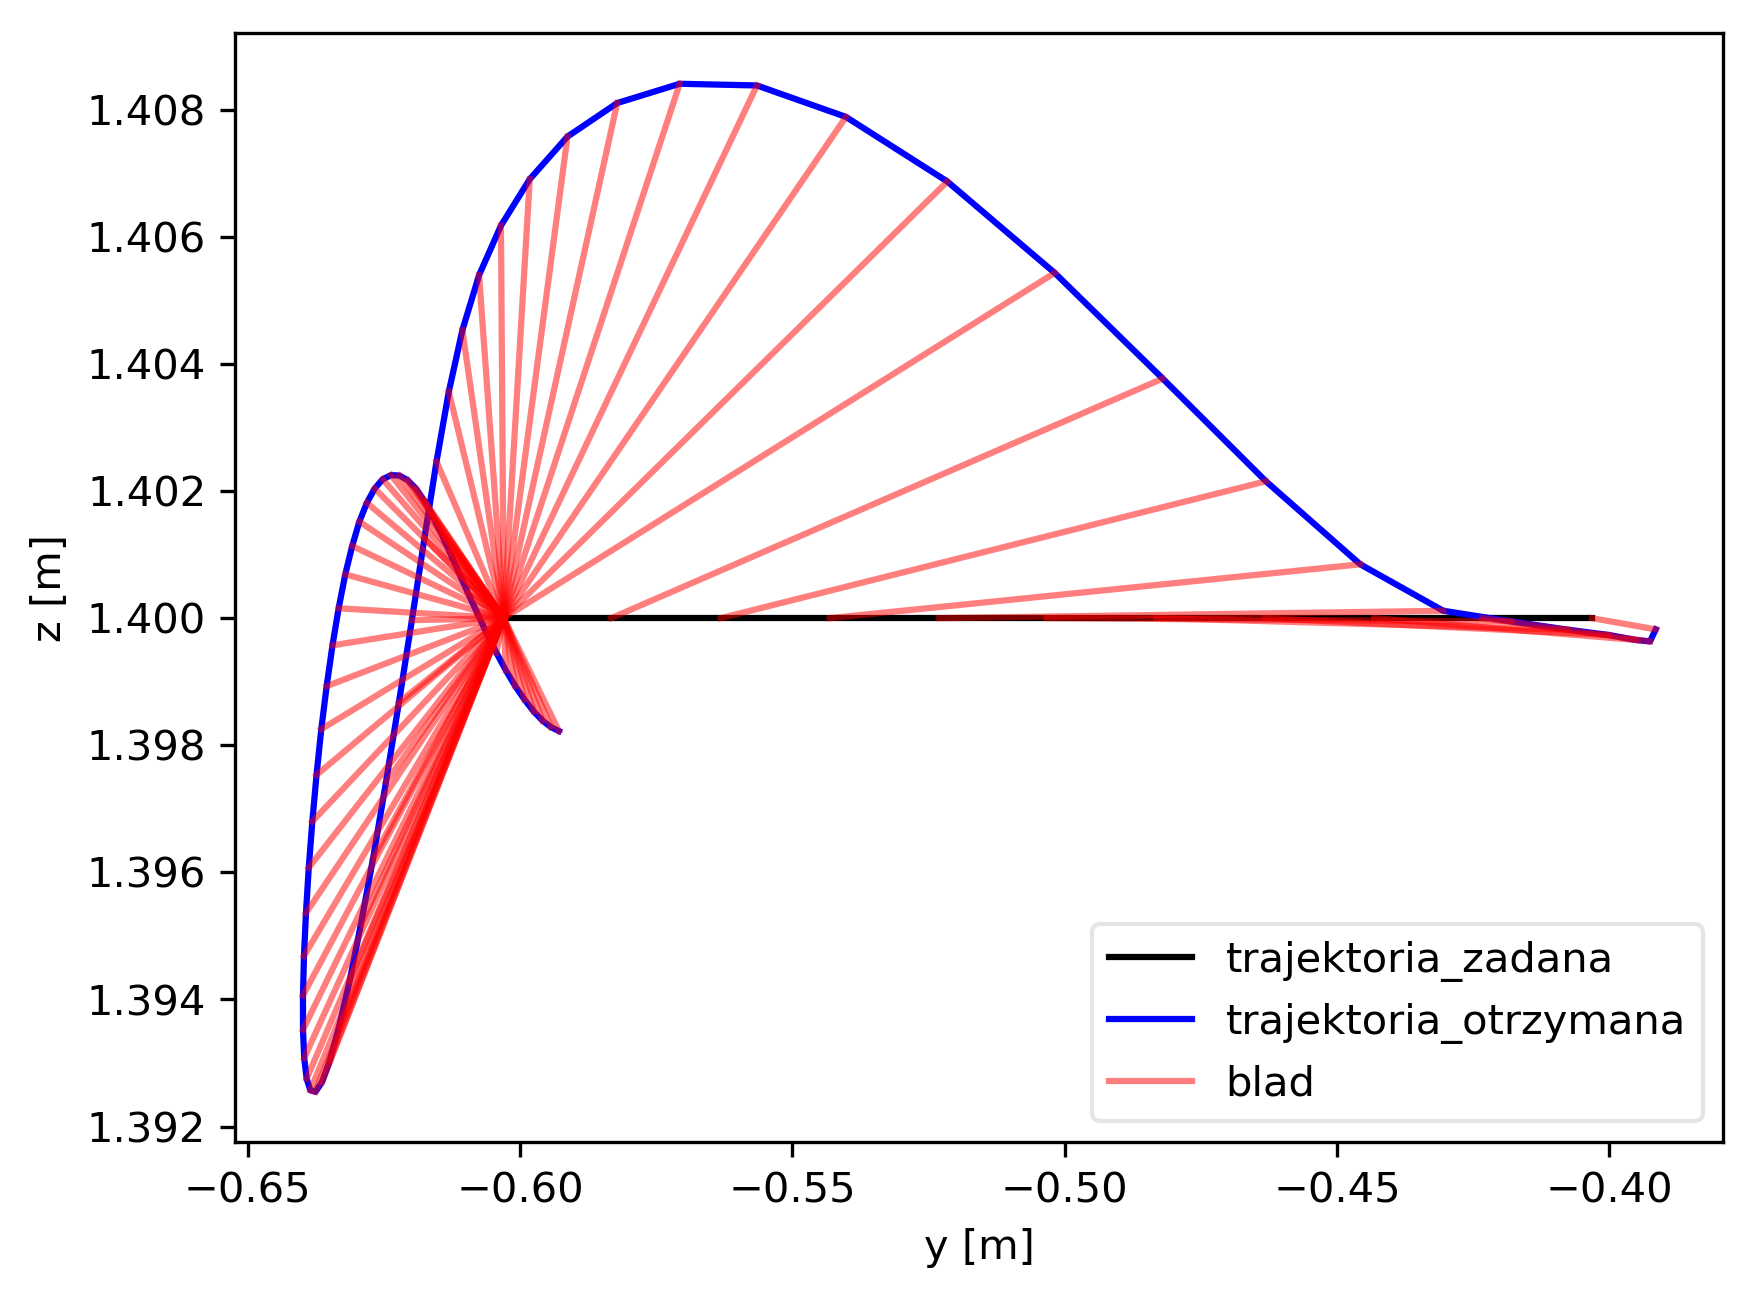
\includegraphics[width=.45\textwidth]{../../velma/przerobione_testy/out/w_bok_miekki/yz_ate_plot_podnoszenie_miekki_komp_wiertarka.png}
	}
	\caption{Ruch w~bok. Porównanie trajektorii chwytaka w~osiach $Y$ i~$Z$}
	\label{fig:w_bok_miekki_porow_przedm}
\end{figure}


% \begin{figure}
% 	\centering
% 	\subfigure[Brak algorytmu kompensacji]{
% 		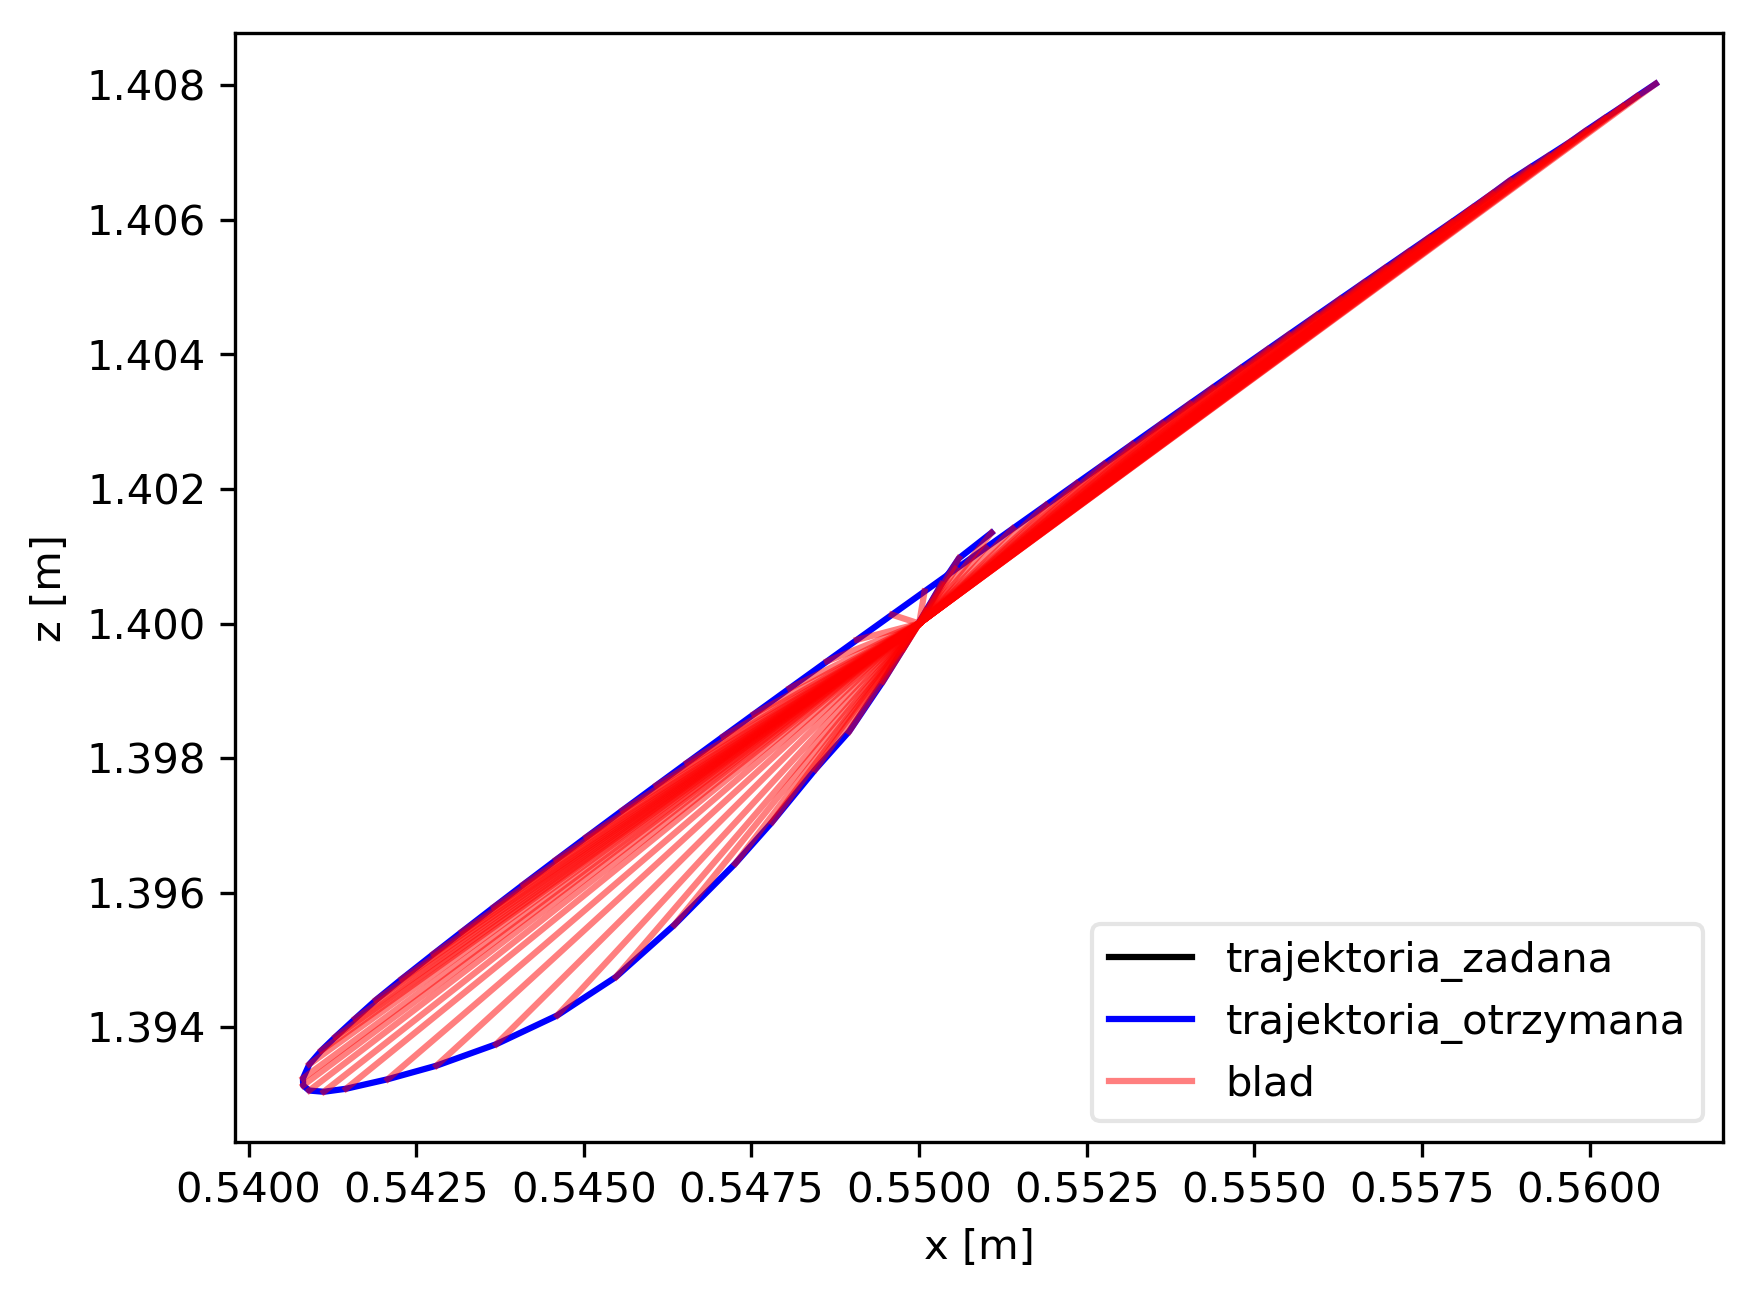
\includegraphics[width=.45\textwidth]{../../velma/przerobione_testy/out/w_bok_miekki/xz_ate_plot_podnoszenie_miekki_bez_brak.png}
% 	}
% 	\hfill
% 	\subfigure[Zalaczony algorytm kompnesacji]{
% 		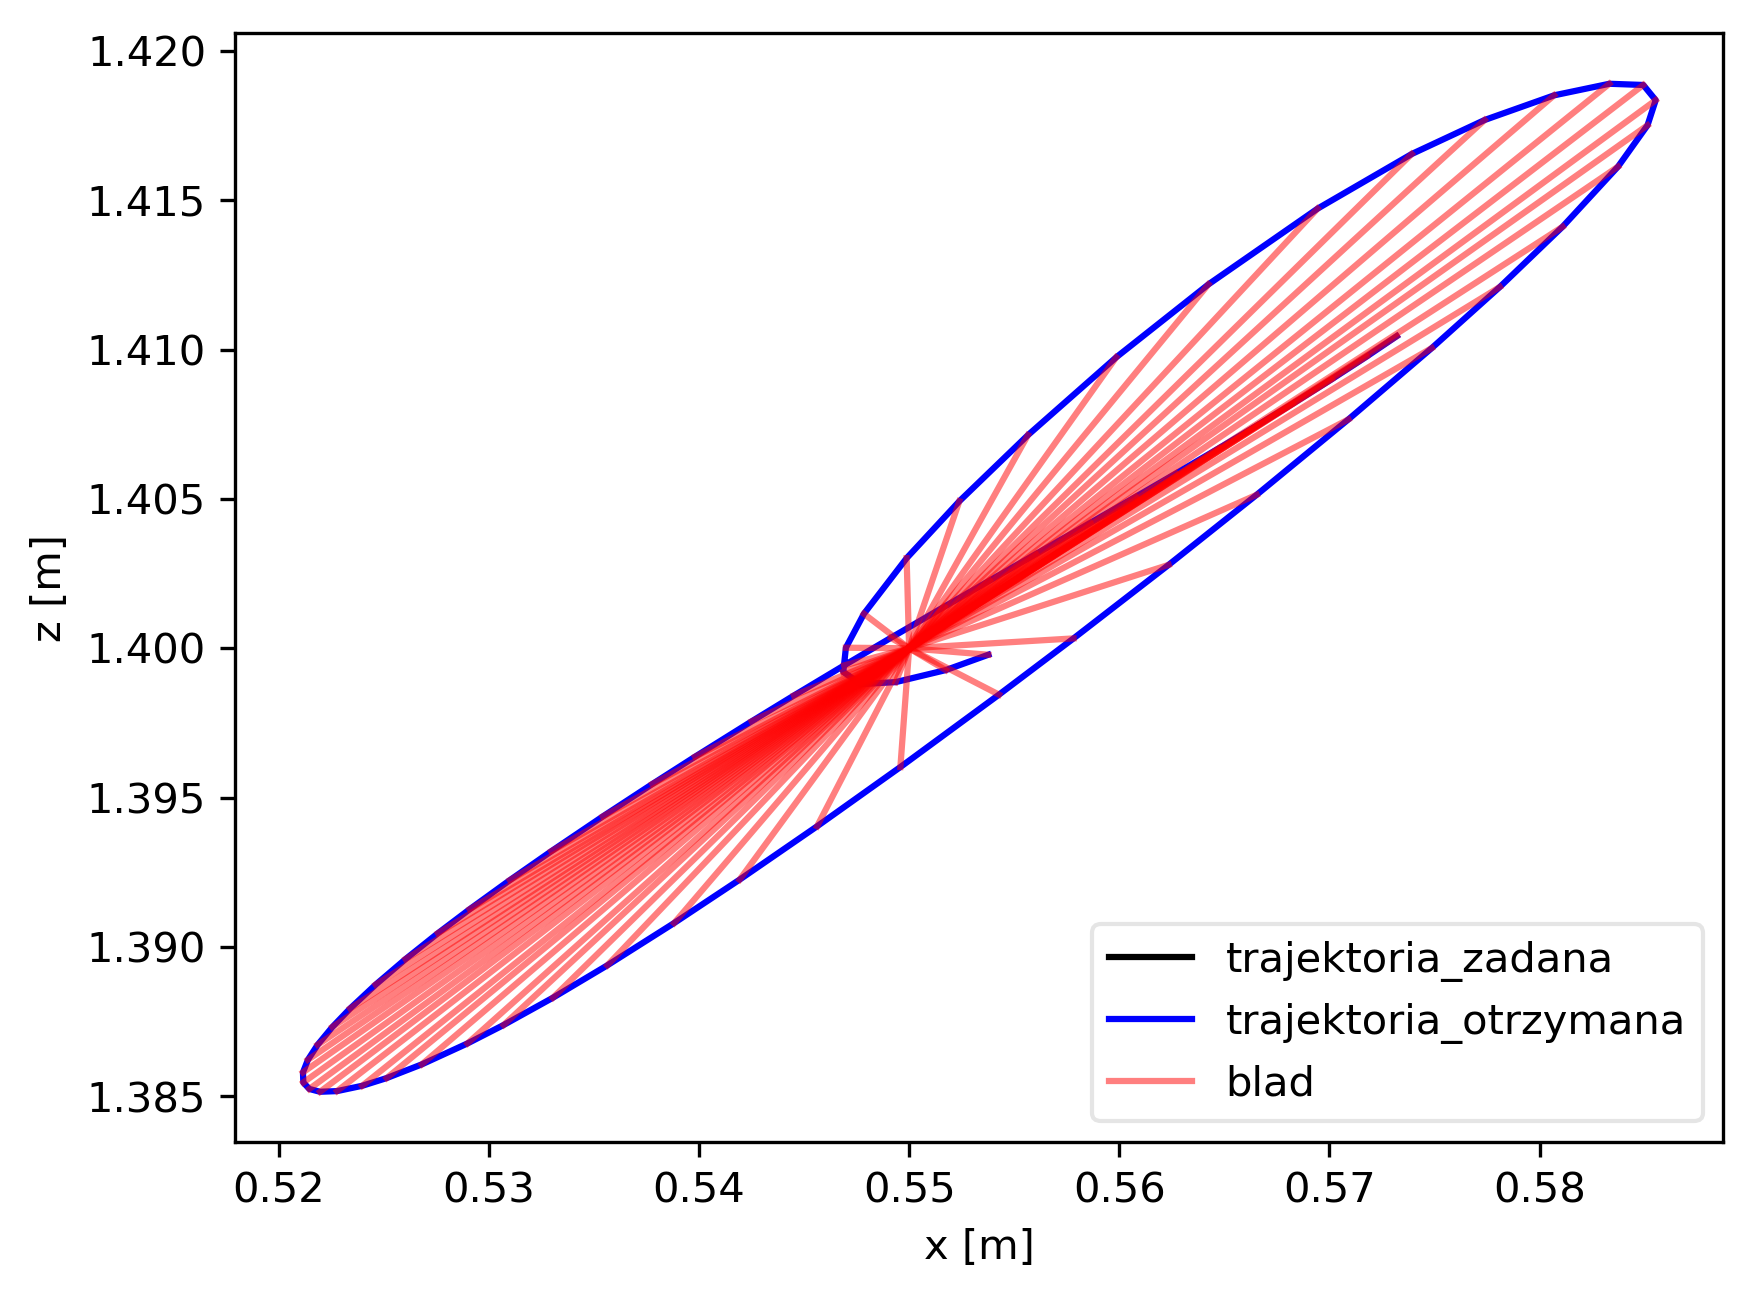
\includegraphics[width=.45\textwidth]{../../velma/przerobione_testy/out/w_bok_miekki/xz_ate_plot_podnoszenie_miekki_komp_brak.png}
% 	}
% 	\caption{Porównanie trajektorii chwytaka w~osiach $X$ i~$Z$}
% 	\label{fig:w_bok_miekki_porow_komp_bok}
% \end{figure}

% \begin{figure}
% 	\centering
% 	\subfigure[Trajektoria z~chwycona puszka]{
% 		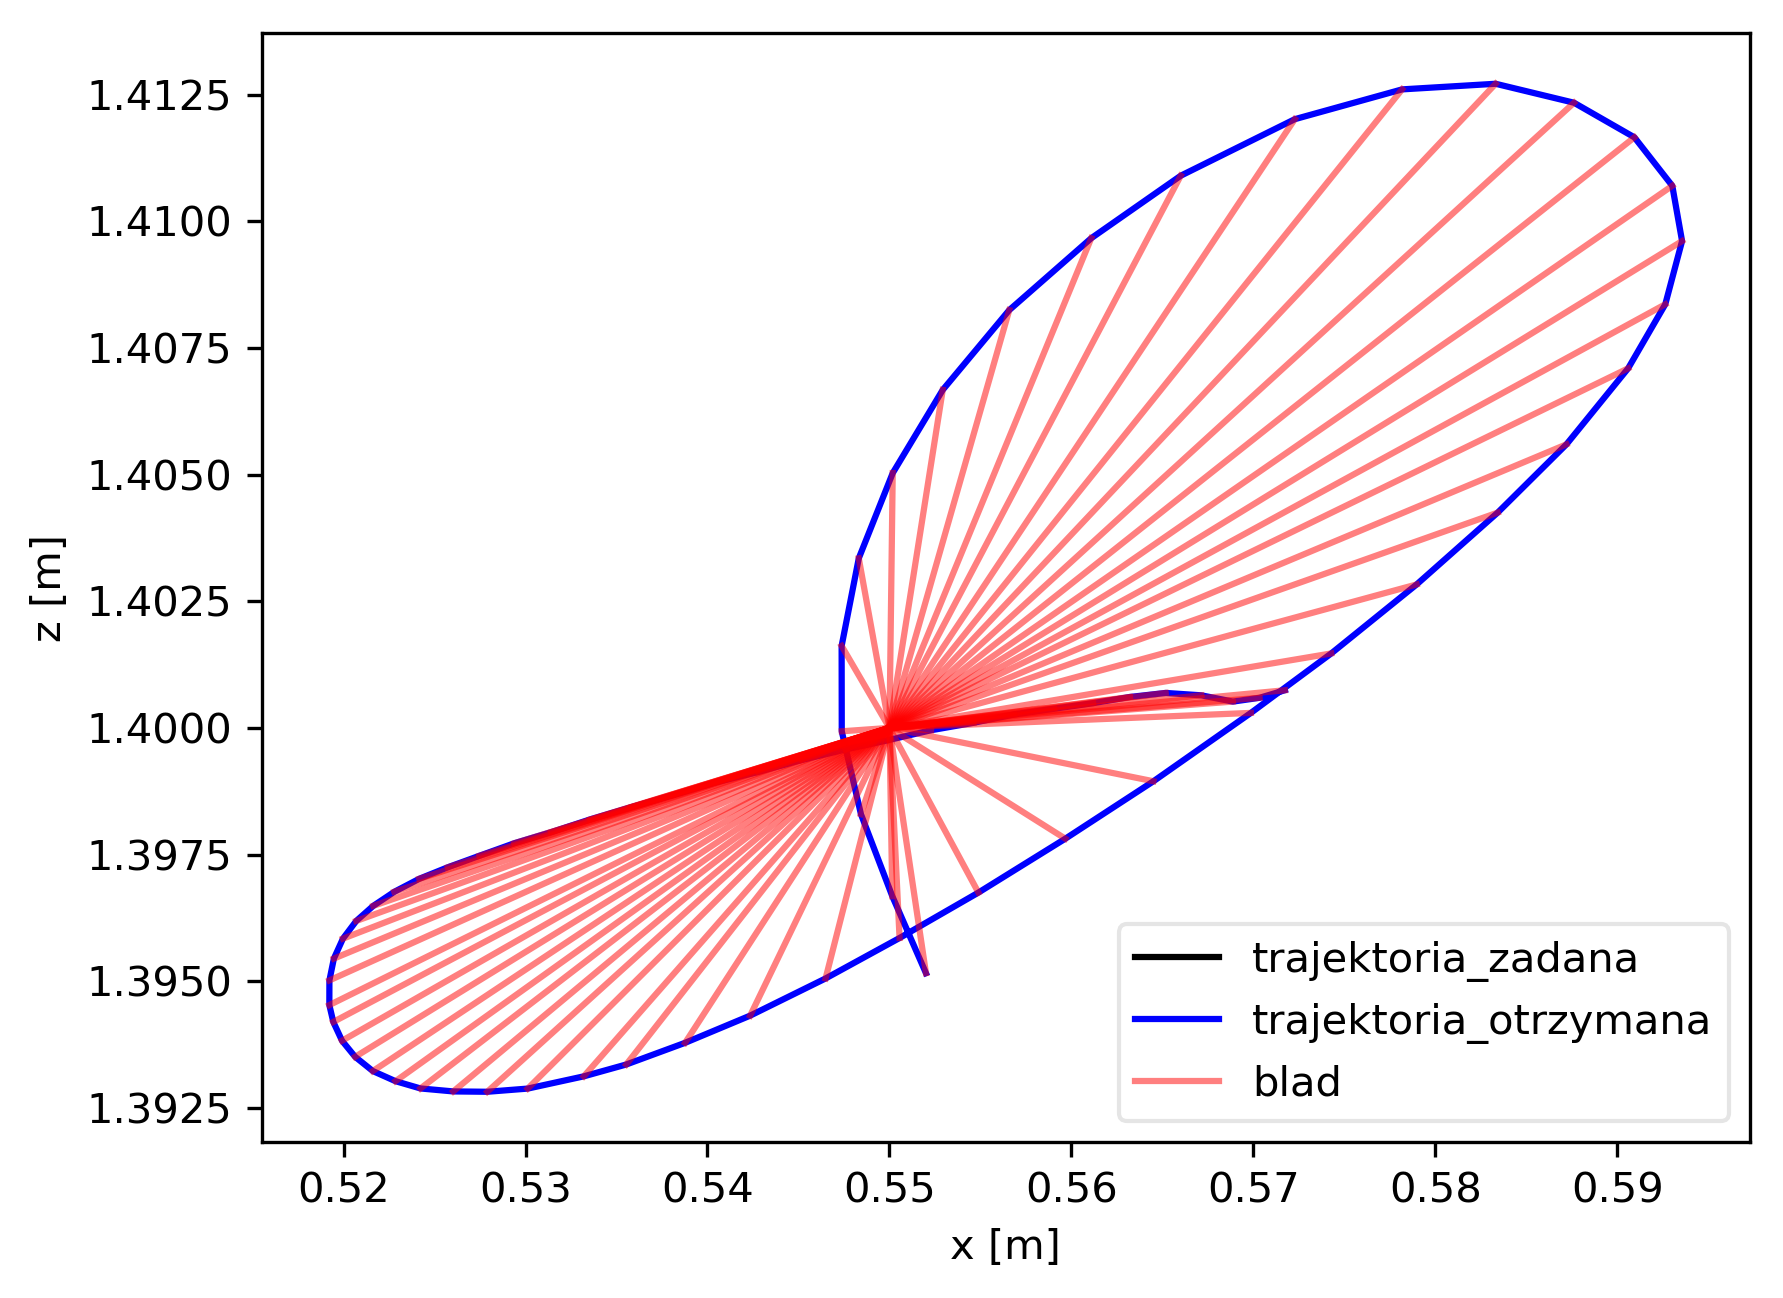
\includegraphics[width=.45\textwidth]{../../velma/przerobione_testy/out/w_bok_miekki/xz_ate_plot_podnoszenie_miekki_komp_piwo.png}
% 	}
% 	\hfill
% 	\subfigure[Trajektoria z~chwycona wiertarka]{
% 		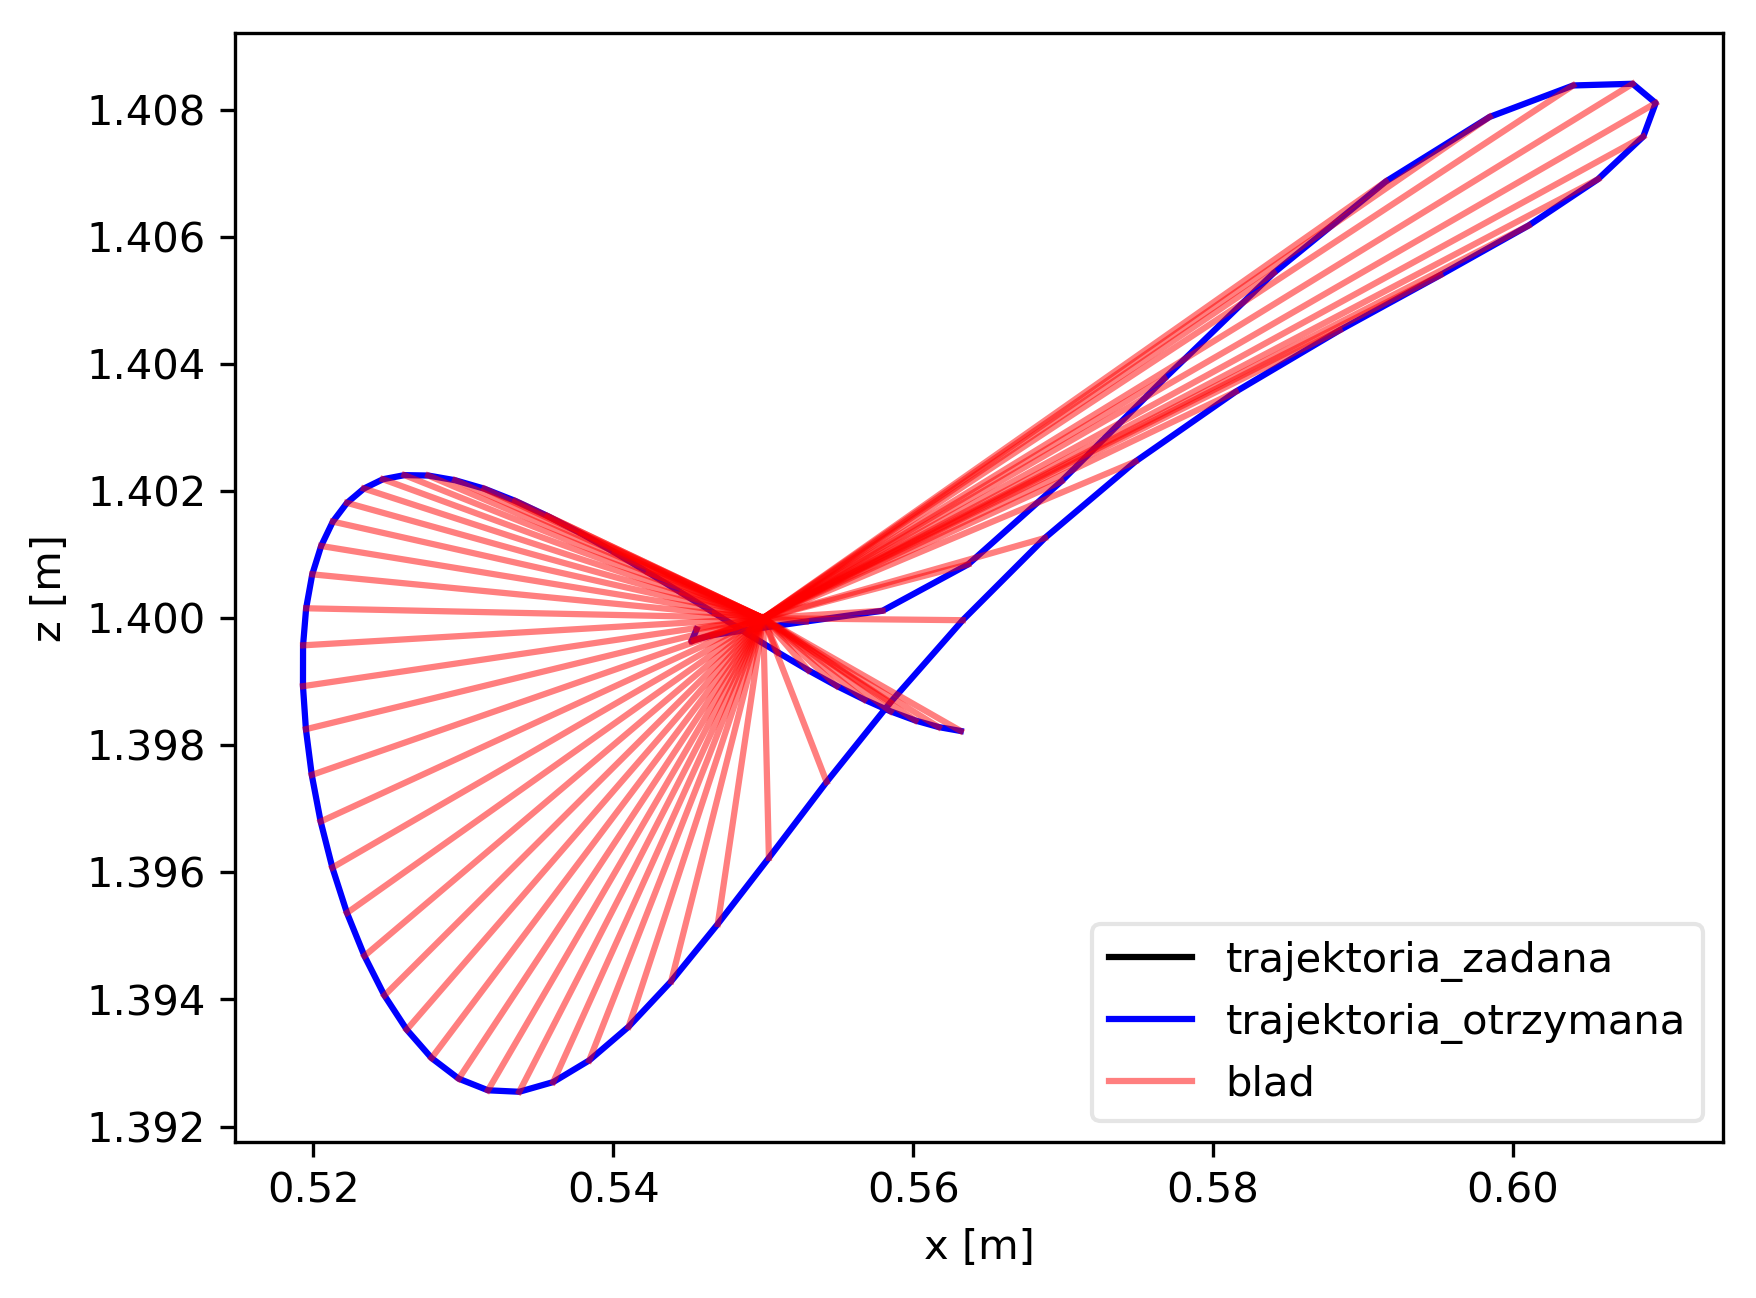
\includegraphics[width=.45\textwidth]{../../velma/przerobione_testy/out/w_bok_miekki/xz_ate_plot_podnoszenie_miekki_komp_wiertarka.png}
% 	}
% 	\caption{Porównanie trajektorii chwytaka w~osiach $X$ i~$Z$}
% 	\label{fig:w_bok_miekki_porow_przedm_bok}
% \end{figure}

% \begin{figure}[H]
% 	\centering
% 	\subfigure[Rzut na wprost]{
% 		\label{fig:w_bok_miekki_porow_zbiorcze_a}
% 		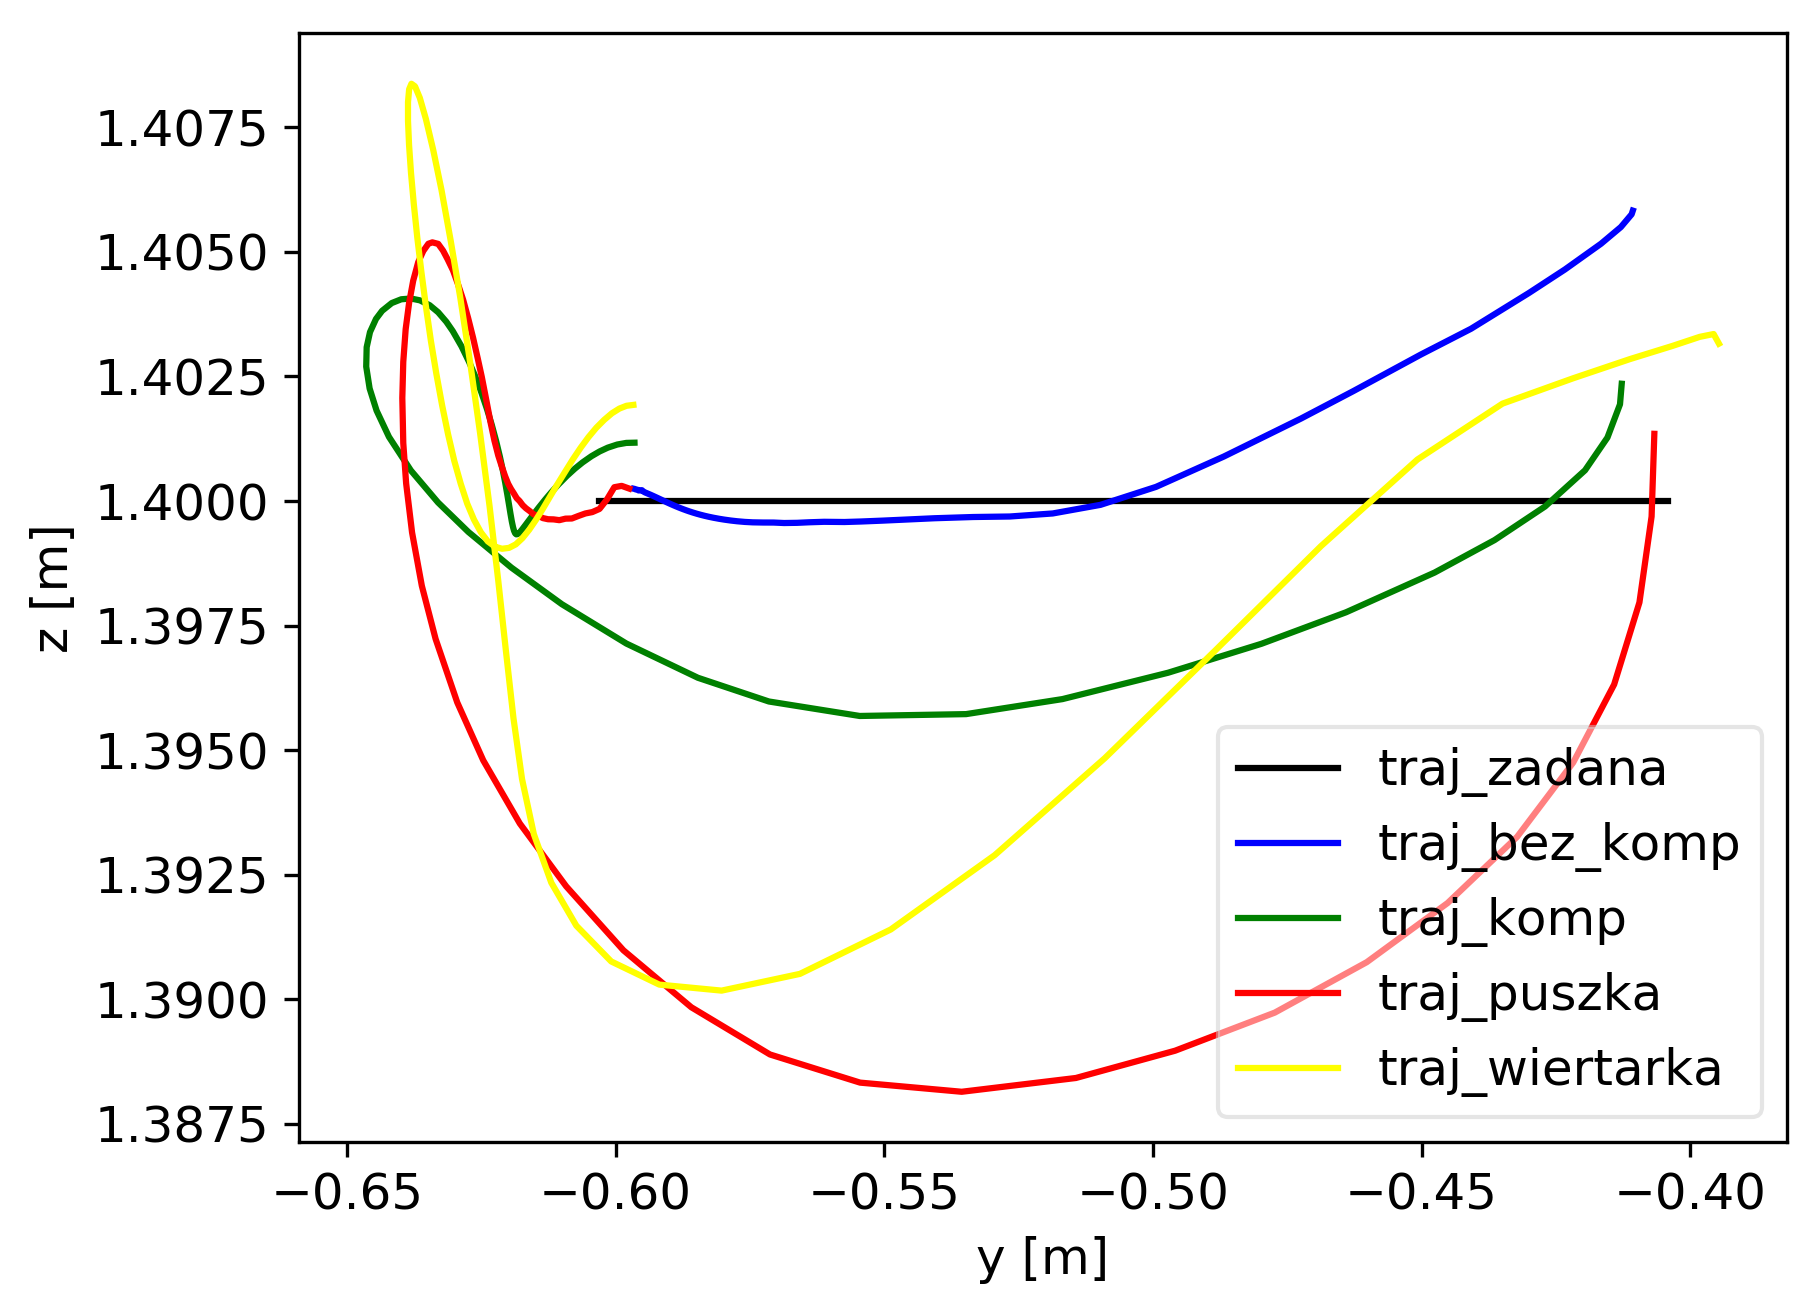
\includegraphics[width=.45\textwidth]{../../velma/przerobione_testy/out/w_bok_miekki/common_yz.png}
% 	}
% 	\hfill
% 	% \subfigure[Rzut z~boku]{
% 	% 	\label{fig:w_bok_miekki_porow_zbiorcze_b}
% 	% 	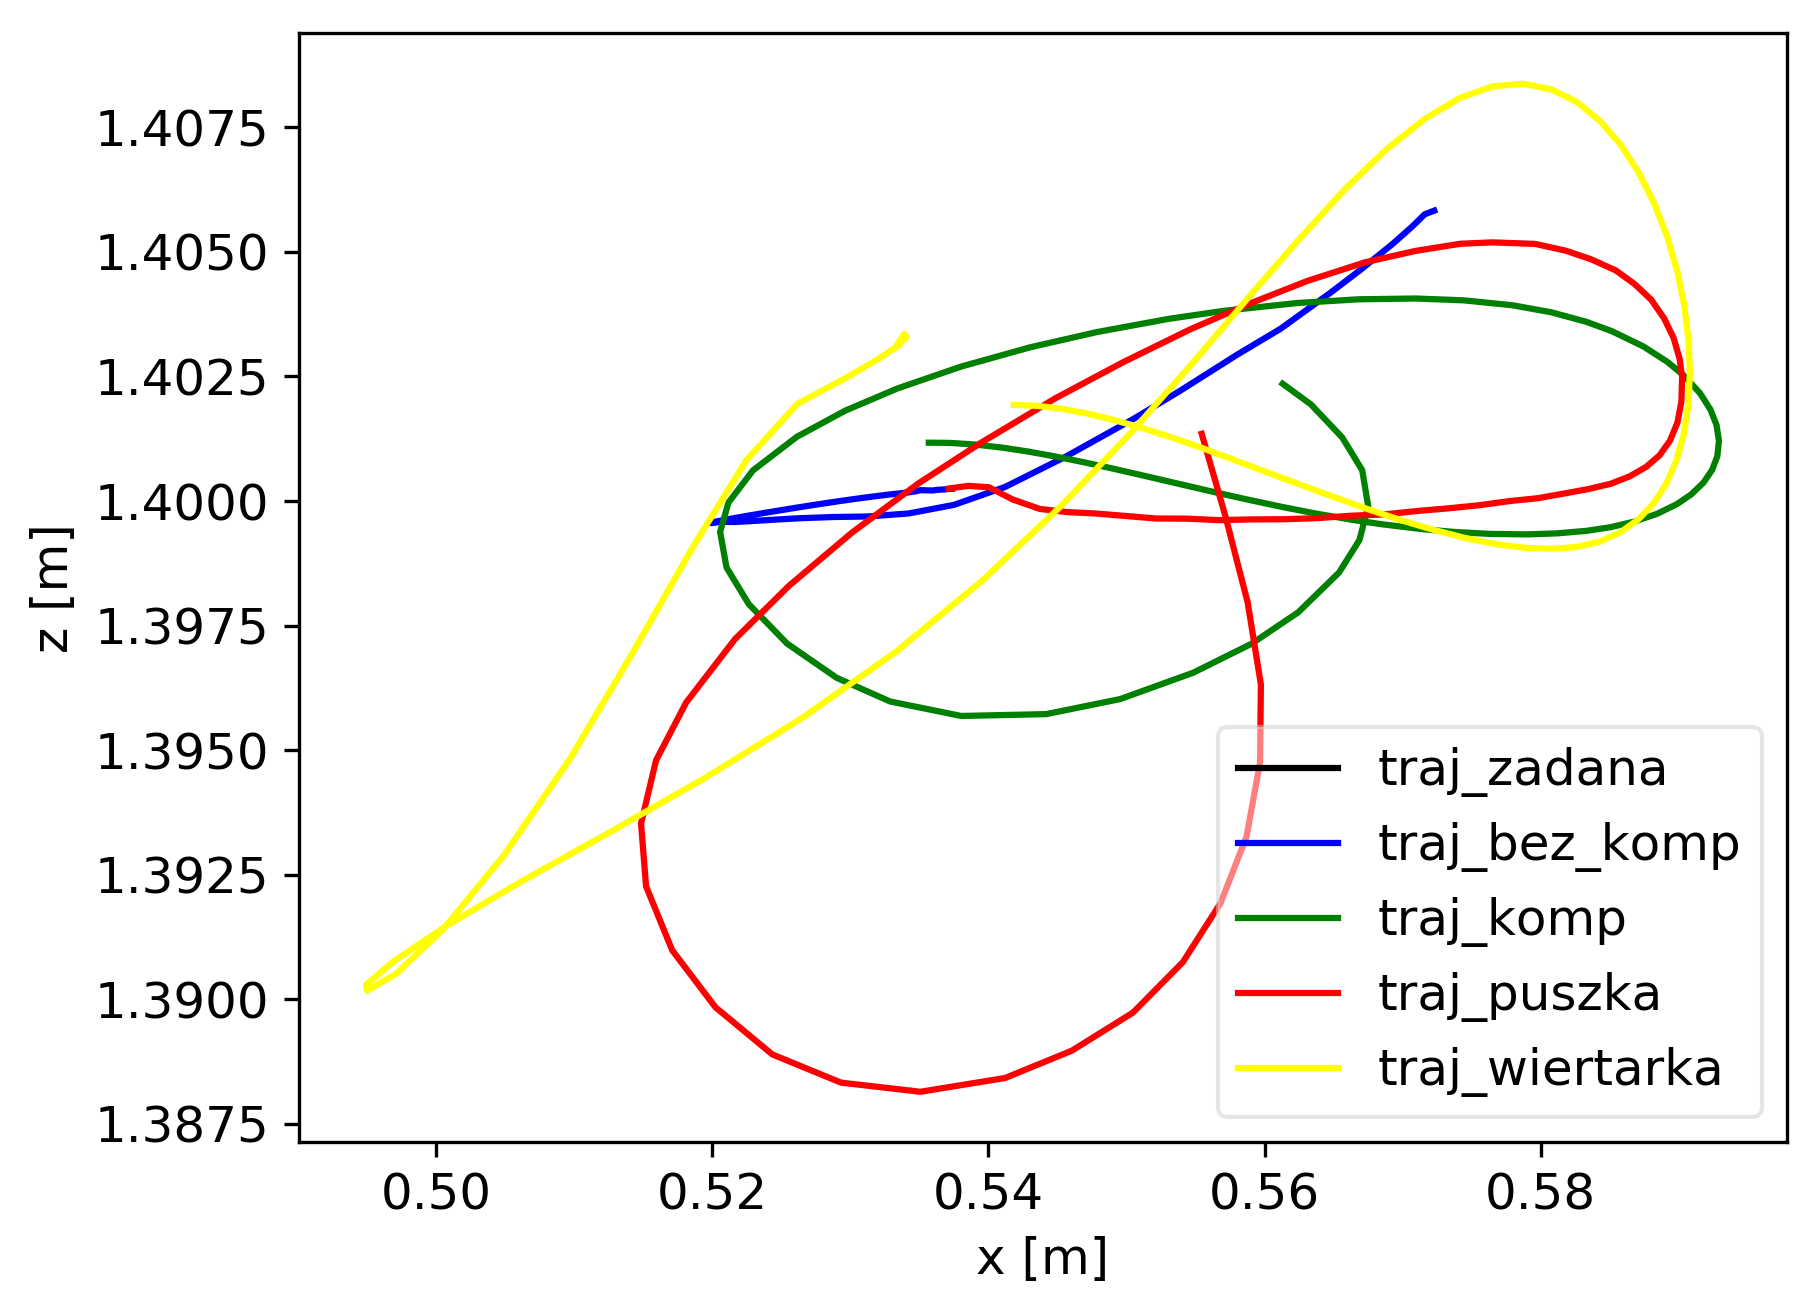
\includegraphics[width=.45\textwidth]{../../velma/przerobione_testy/out/w_bok_miekki/common_xz.png}
% 	% }
% 	\caption{Porównanie wszystkich trajektorii.}
% 	\label{fig:w_bok_miekki_porow_zbiorcze}
% \end{figure}


\section{Ruch do góry}

Eksperyment ma przetestować zachowanie algorytmu kompensacji przy ruchu końcówki do góry (rys. \ref{fig:do_gory_a}, \ref{fig:do_gory_rot}).  Ruch jest interesujący przez działanie siły grawitacji właśnie w~tej osi. Ruch różni się od ruchu podnoszenia przedmiotu, ponieważ grawitacja przedmiotu jest już wstępnie skompensowana. Trajektoria ruchu w~rzucie ATE została zaprezentowana na rys. \ref{fig:do_gory_porow_komp}, \ref{fig:do_gory_porow_przedm}.

\begin{figure}[H]
	\centering
	\subfigure[Oś $X$]{
		\label{fig:do_gory_ax}
		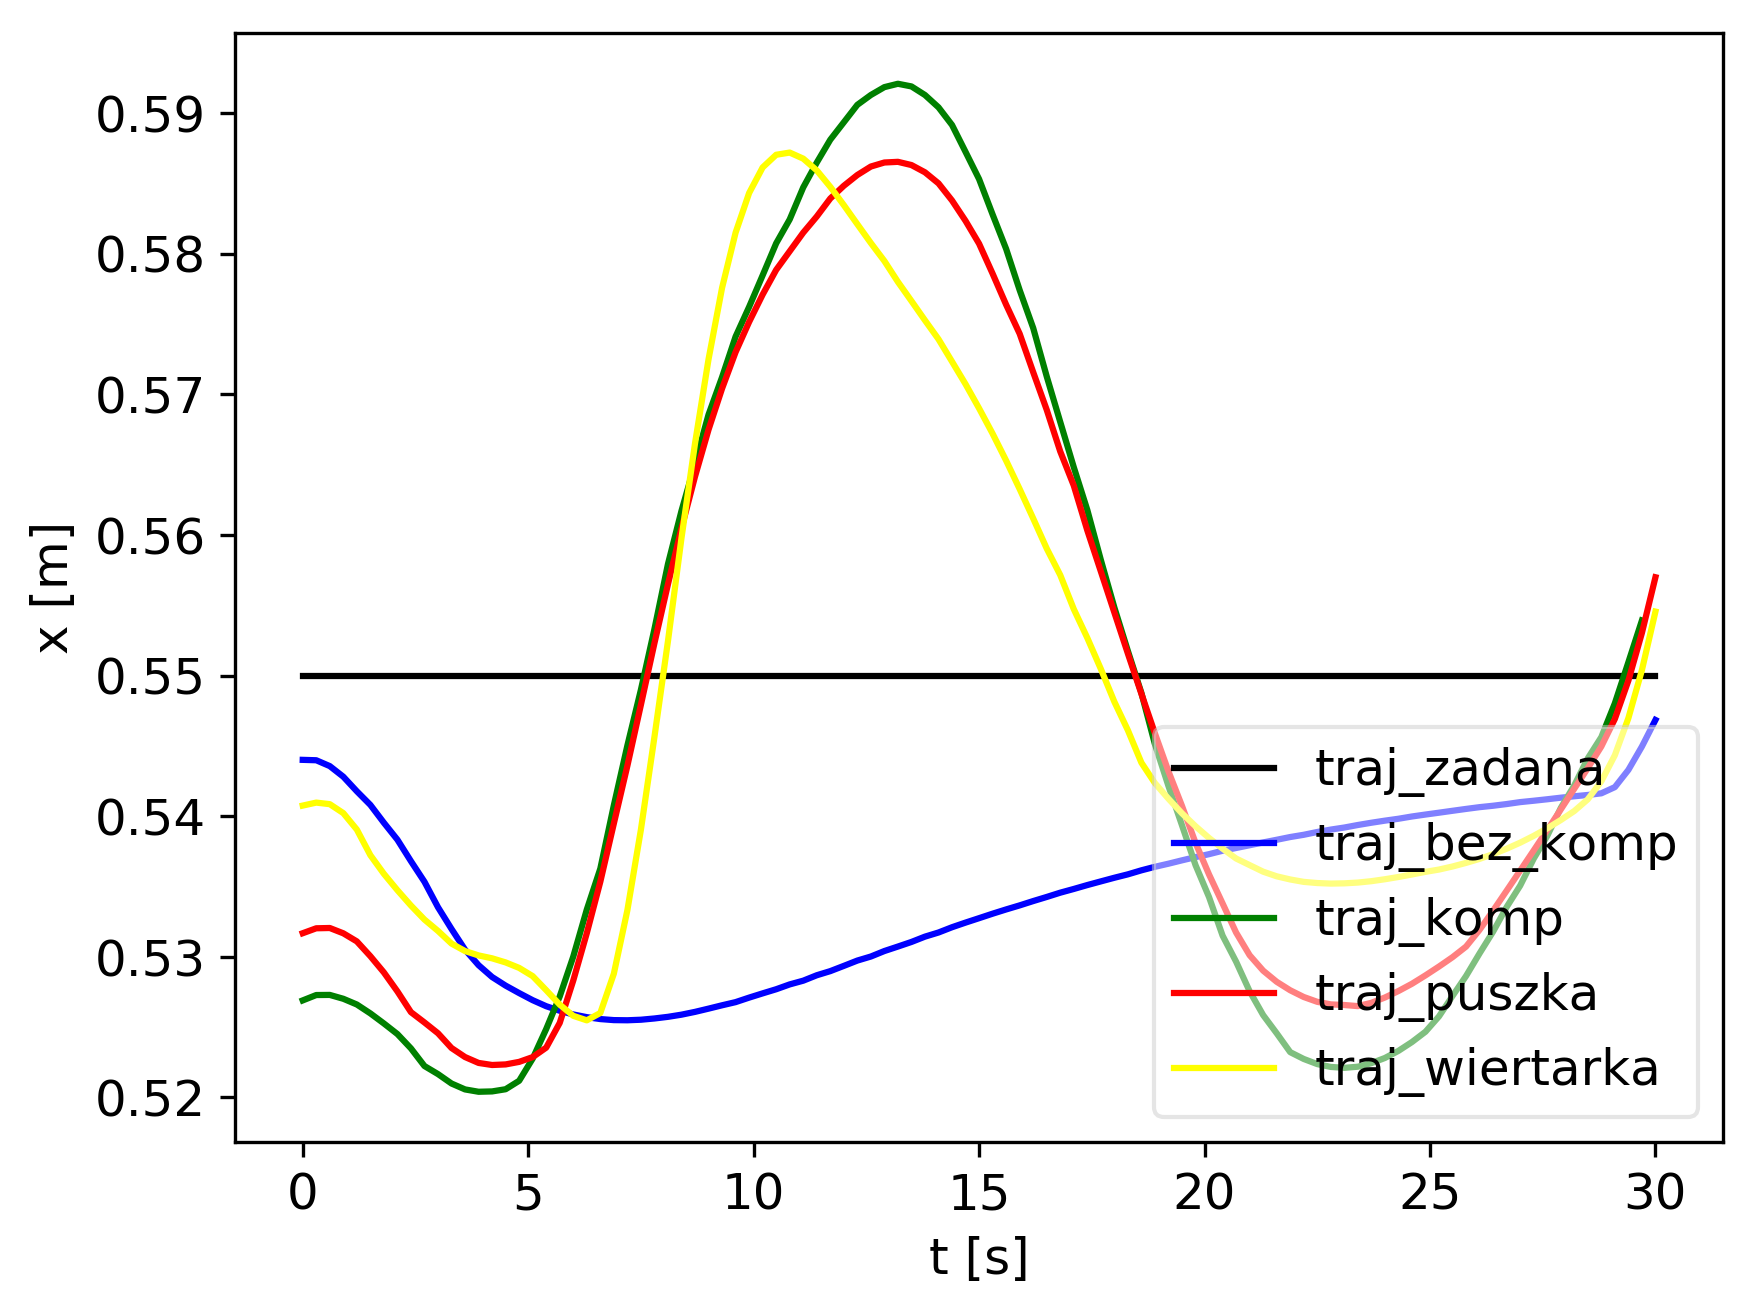
\includegraphics[width=.45\textwidth]{../../velma/przerobione_testy/out/do_gory/common_ax.png}
	}
	\hfill
	\subfigure[Oś $Y$]{
		\label{fig:do_gory_ay}
		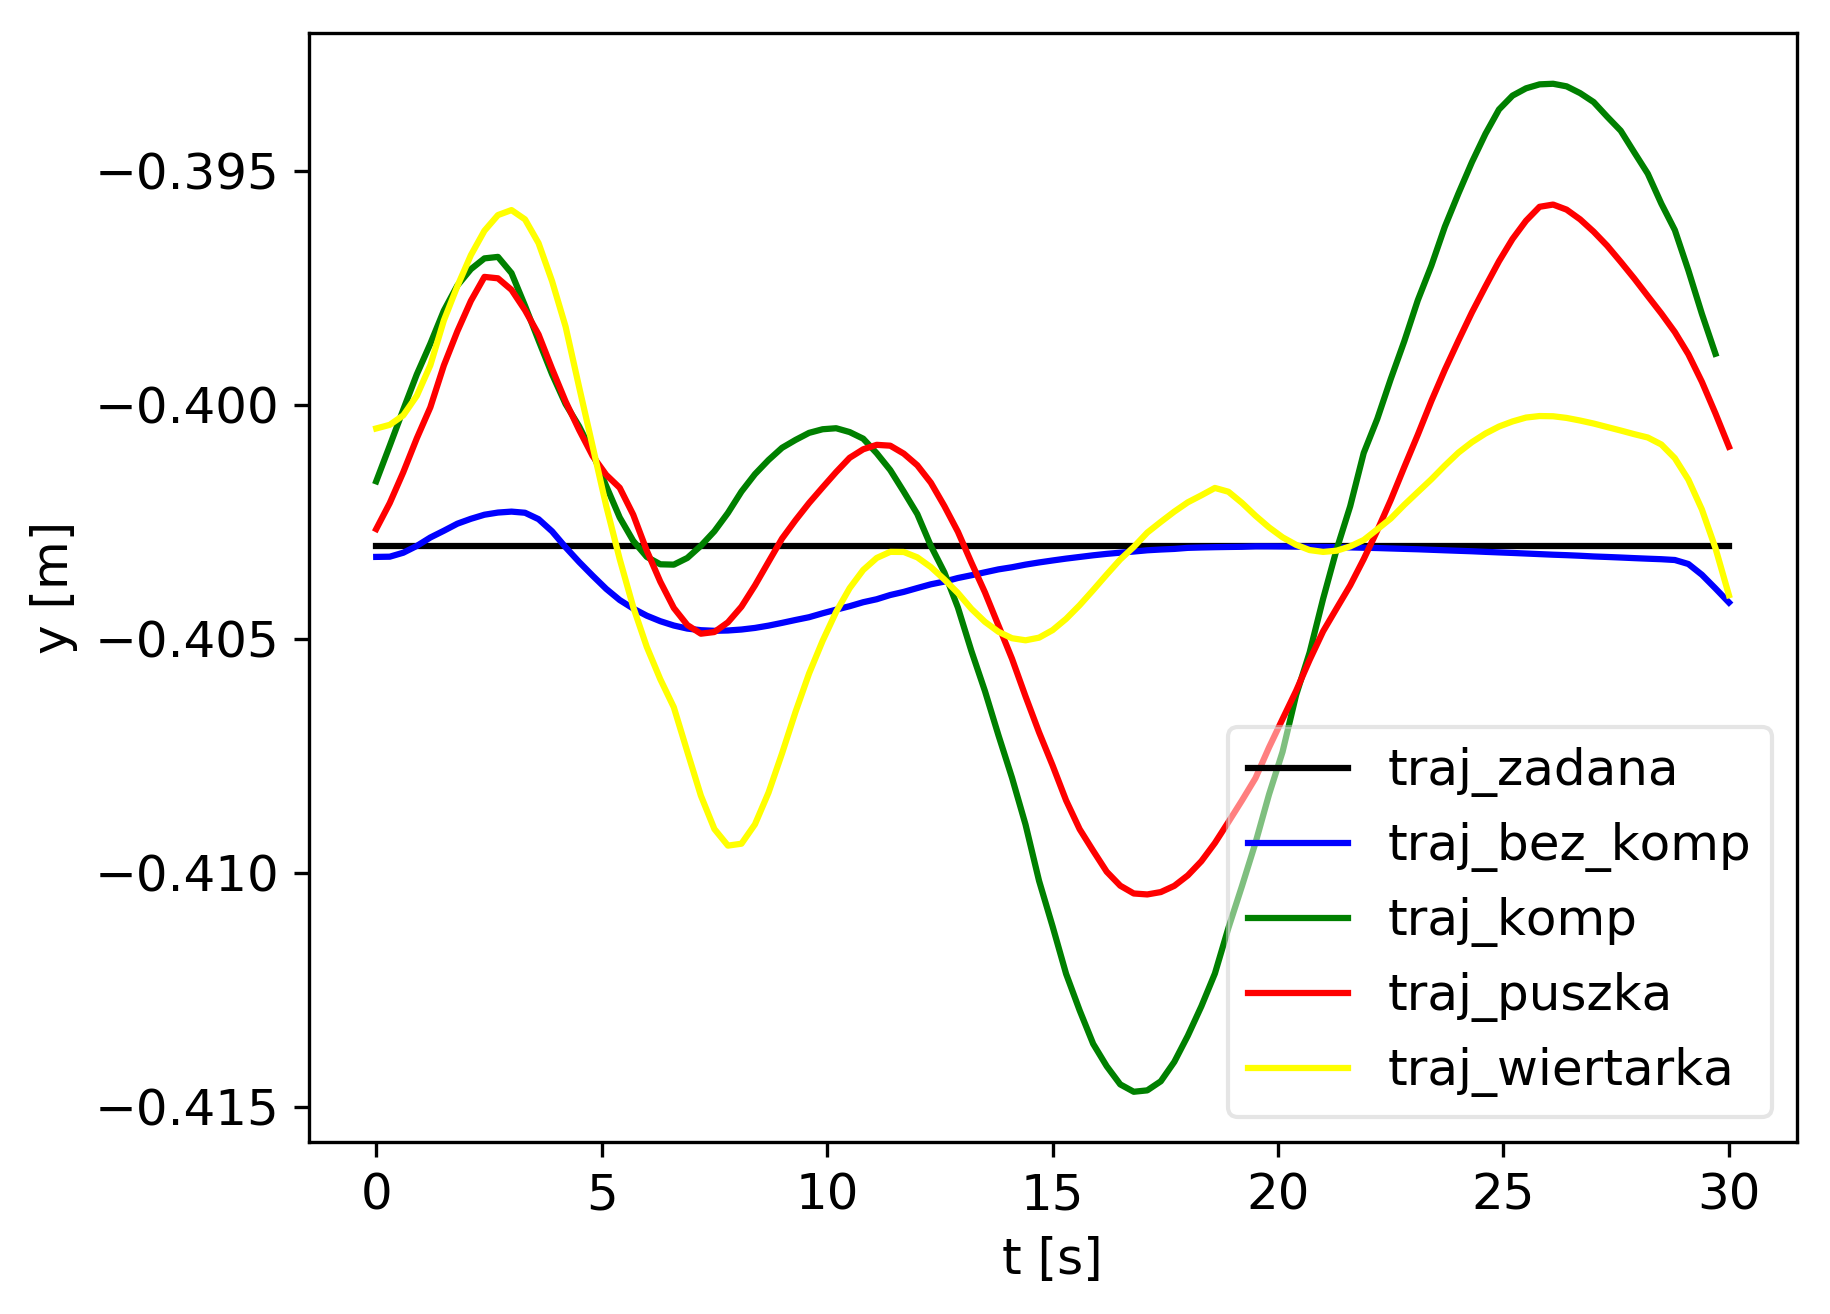
\includegraphics[width=.45\textwidth]{../../velma/przerobione_testy/out/do_gory/common_ay.png}
	}
	
	\subfigure[Oś $Z$]{
		\label{fig:do_gory_az}
		\includegraphics[width=.45\textwidth]{../../velma/przerobione_testy/out/do_gory/common_az.png}
	}

	\caption{Ruch do góry. Porównanie trajektorii pozycji w~zależności od czasu.}
	\label{fig:do_gory_a}

\end{figure}
\begin{figure}[H]
	\centering
	\subfigure[Brak algorytmu kompensacji]{
		\includegraphics[width=.45\textwidth]{../../velma/przerobione_testy/out/do_gory/xz_ate_plot_podnoszenie_miekki_bez_brak.png}
	}
	\hfill
	\subfigure[Zalaczony algorytm kompnesacji]{
		\includegraphics[width=.45\textwidth]{../../velma/przerobione_testy/out/do_gory/xz_ate_plot_podnoszenie_miekki_komp_brak.png}
	}
	\caption{Ruch do góry. Porównanie trajektorii chwytaka w~osiach $X$ i~$Z$}
	\label{fig:do_gory_porow_komp}
\end{figure}


\begin{figure}[H]
	\centering
	\subfigure[Kąt osi $X$]{
		\label{fig:do_gory_rotx}
		\includegraphics[width=.45\textwidth]{../../velma/przerobione_testy/out/do_gory/common_rotx.png}
	}
	\hfill
	\subfigure[Kąt osi $Y$]{
		\label{fig:do_gory_roty}
		\includegraphics[width=.45\textwidth]{../../velma/przerobione_testy/out/do_gory/common_roty.png}
	}
	
	\subfigure[Kąt osi $Z$]{
		\label{fig:do_gory_rotz}
		\includegraphics[width=.45\textwidth]{../../velma/przerobione_testy/out/do_gory/common_rotz.png}
	}

	\caption{Ruch do góry. Porównanie trajektorii kątów w~notacji Eulera w~zależności od czasu.}
	\label{fig:do_gory_rot}

\end{figure}



\begin{figure}[H]
	\centering
	\subfigure[Trajektoria z~chwycona puszka]{
		\includegraphics[width=.45\textwidth]{../../velma/przerobione_testy/out/do_gory/xz_ate_plot_podnoszenie_miekki_komp_piwo.png}
	}
	\hfill
	\subfigure[Trajektoria z~chwycona wiertarka]{
		\includegraphics[width=.45\textwidth]{../../velma/przerobione_testy/out/do_gory/xz_ate_plot_podnoszenie_miekki_komp_wiertarka.png}
	}
	\caption{Ruch do góry. Porównanie trajektorii chwytaka w~osiach $X$ i~$Z$}
	\label{fig:do_gory_porow_przedm}
\end{figure}


% \begin{figure}
% 	\centering
% 	\subfigure[Brak algorytmu kompensacji]{
% 		\includegraphics[width=.45\textwidth]{../../velma/przerobione_testy/out/do_gory/xy_ate_plot_podnoszenie_miekki_bez_brak.png}
% 	}
% 	\hfill
% 	\subfigure[Zalaczony algorytm kompnesacji]{
% 		\includegraphics[width=.45\textwidth]{../../velma/przerobione_testy/out/do_gory/xy_ate_plot_podnoszenie_miekki_komp_brak.png}
% 	}
% 	\caption{Porównanie trajektorii chwytaka w~osiach $X$ i~$Y$}
% 	\label{fig:do_gory_porow_komp_bok}
% \end{figure}

% \begin{figure}
% 	\centering
% 	\subfigure[Trajektoria z~chwycona puszka]{
% 		\includegraphics[width=.45\textwidth]{../../velma/przerobione_testy/out/do_gory/xy_ate_plot_podnoszenie_miekki_komp_piwo.png}
% 	}
% 	\hfill
% 	\subfigure[Trajektoria z~chwycona wiertarka]{
% 		\includegraphics[width=.45\textwidth]{../../velma/przerobione_testy/out/do_gory/xy_ate_plot_podnoszenie_miekki_komp_wiertarka.png}
% 	}
% 	\caption{Porównanie trajektorii chwytaka w~osiach $X$ i~$Y$}
% 	\label{fig:do_gory_porow_przedm_bok}
% \end{figure}

% \begin{figure}[H]
% 	\centering
% 	\subfigure[Rzut na wprost]{
% 		\label{fig:do_gory_porow_zbiorcze_a}
% 		\includegraphics[width=.45\textwidth]{../../velma/przerobione_testy/out/do_gory/common_xz.png}
% 	}
% 	% \hfill
% 	% \subfigure[Rzut z~gory]{
% 	% 	\label{fig:do_gory_porow_zbiorcze_b}
% 	% 	\includegraphics[width=.45\textwidth]{../../velma/przerobione_testy/out/do_gory/common_xy.png}
% 	% }
% 	\caption{Porównanie wszystkich trajektorii.}
% 	\label{fig:do_gory_porow_zbiorcze}
% \end{figure}

\section{Ruch do dołu}

Eksperyment ma przetestować zachowanie algorytmu kompensacji przy ruchu końcówki do dołu (rys. \ref{fig:do_dolu_a}, \ref{fig:do_dolu_rot}). Trajektoria ruchu pokrywa się z osią w której działa siła grawitacji Trajektoria ruchu w~rzucie ATE została zaprezentowana na rys. \ref{fig:do_dolu_porow_komp}, \ref{fig:do_dolu_porow_przedm}.
% Trajektoria widoczna z~boku (w osiach $X$ oraz $Z$) została zaprezentowana na rys. \ref{fig:do_dolu_porow_komp_bok}, \ref{fig:do_dolu_porow_przedm_bok} i~\ref{fig:do_dolu_porow_zbiorcze_b}.

\begin{figure}[H]
	\centering
	\subfigure[Oś $X$]{
		\label{fig:do_dolu_ax}
		\includegraphics[width=.45\textwidth]{../../velma/przerobione_testy/out/do_dolu/common_ax.png}
	}
	\hfill
	\subfigure[Oś $Y$]{
		\label{fig:do_dolu_ay}
		\includegraphics[width=.45\textwidth]{../../velma/przerobione_testy/out/do_dolu/common_ay.png}
	}
	
	\subfigure[Oś $Z$]{
		\label{fig:do_dolu_az}
		\includegraphics[width=.45\textwidth]{../../velma/przerobione_testy/out/do_dolu/common_az.png}
	}

	\caption{Ruch do dołu. Porównanie trajektorii pozycji w~zależności od czasu.}
	\label{fig:do_dolu_a}

\end{figure}

\begin{figure}[H]
	\centering
	\subfigure[Brak algorytmu kompensacji]{
		\includegraphics[width=.45\textwidth]{../../velma/przerobione_testy/out/do_dolu/xz_ate_plot_podnoszenie_miekki_bez_brak.png}
	}
	\hfill
	\subfigure[Zalaczony algorytm kompnesacji]{
		\includegraphics[width=.45\textwidth]{../../velma/przerobione_testy/out/do_dolu/xz_ate_plot_podnoszenie_miekki_komp_brak.png}
	}
	\caption{Ruch do dołu. Porównanie trajektorii chwytaka w~osiach $X$ i~$Z$}
	\label{fig:do_dolu_porow_komp}
\end{figure}

\begin{figure}[H]
	\centering
	\subfigure[Kąt osi $X$]{
		\label{fig:do_dolu_rotx}
		\includegraphics[width=.45\textwidth]{../../velma/przerobione_testy/out/do_dolu/common_rotx.png}
	}
	\hfill
	\subfigure[Kąt osi $Y$]{
		\label{fig:do_dolu_roty}
		\includegraphics[width=.45\textwidth]{../../velma/przerobione_testy/out/do_dolu/common_roty.png}
	}
	
	\subfigure[Kąt osi $Z$]{
		\label{fig:do_dolu_rotz}
		\includegraphics[width=.45\textwidth]{../../velma/przerobione_testy/out/do_dolu/common_rotz.png}
	}

	\caption{Ruch do dołu. Porównanie trajektorii katów w~notacji Eulera w~zależności od czasu.}
	\label{fig:do_dolu_rot}

\end{figure}



\begin{figure}[H]
	\centering
 	\subfigure[Trajektoria z~chwycona puszka]{
 		\includegraphics[width=.45\textwidth]{../../velma/przerobione_testy/out/do_dolu/xz_ate_plot_podnoszenie_miekki_komp_piwo.png}
	}
 	\hfill
 	\subfigure[Trajektoria z~chwycona wiertarka]{
 		\includegraphics[width=.45\textwidth]{../../velma/przerobione_testy/out/do_dolu/xz_ate_plot_podnoszenie_miekki_komp_wiertarka.png}
 	}
 	\caption{Porównanie trajektorii chwytaka w~osiach $X$ i~$Z$}
 	\label{fig:do_dolu_porow_przedm}
 \end{figure}


% \begin{figure}
% 	\centering
% 	\subfigure[Brak algorytmu kompensacji]{
% 		\includegraphics[width=.45\textwidth]{../../velma/przerobione_testy/out/do_dolu/xy_ate_plot_podnoszenie_miekki_bez_brak.png}
% 	}
% 	\hfill
% 	\subfigure[Zalaczony algorytm kompnesacji]{
% 		\includegraphics[width=.45\textwidth]{../../velma/przerobione_testy/out/do_dolu/xy_ate_plot_podnoszenie_miekki_komp_brak.png}
% 	}
% 	\caption{Porównanie trajektorii chwytaka w~osiach $X$ i~$Y$}
% 	\label{fig:do_dolu_porow_komp_bok}
% \end{figure}

% \begin{figure}
% 	\centering
% 	\subfigure[Trajektoria z~chwycona puszka]{
% 		\includegraphics[width=.45\textwidth]{../../velma/przerobione_testy/out/do_dolu/xy_ate_plot_podnoszenie_miekki_komp_piwo.png}
% 	}
% 	\hfill
% 	\subfigure[Trajektoria z~chwycona wiertarka]{
% 		\includegraphics[width=.45\textwidth]{../../velma/przerobione_testy/out/do_dolu/xy_ate_plot_podnoszenie_miekki_komp_wiertarka.png}
% 	}
% 	\caption{Porównanie trajektorii chwytaka w~osiach $X$ i~$Y$}
% 	\label{fig:do_dolu_porow_przedm_bok}
% \end{figure}

% \begin{figure}[H]
% 	\centering
% 	\subfigure[Rzut na wprost]{
% 		\label{fig:do_dolu_porow_zbiorcze_a}
% 		\includegraphics[width=.45\textwidth]{../../velma/przerobione_testy/out/do_dolu/common_xz.png}
% 	}
% 	\hfill
% 	% \subfigure[Rzut z~gory]{
% 	% 	\label{fig:do_dolu_porow_zbiorcze_b}
% 	% 	\includegraphics[width=.45\textwidth]{../../velma/przerobione_testy/out/do_dolu/common_xy.png}
% 	% }
% 	\caption{Porównanie wszystkich trajektorii.}
% 	\label{fig:do_dolu_porow_zbiorcze}
% \end{figure}

\section{Ruch do przodu}

Eksperyment ma przetestować zachowanie algorytmu kompensacji przy ruchu końcówki w~kierunku od robota (rys. \ref{fig:do_przodu_a}, \ref{fig:do_przodu_rot}). Trajektoria ruchu w~rzucie ATE została zaprezentowana na rys. \ref{fig:do_przodu_porow_komp}, \ref{fig:do_przodu_porow_przedm}.
 % i~\ref{fig:do_przodu_porow_zbiorcze_a}. Trajektoria widoczna z~boku (w osiach $X$ oraz $Z$) została zaprezentowana na rys. \ref{fig:do_przodu_porow_komp_bok}, \ref{fig:do_przodu_porow_przedm_bok} i~\ref{fig:do_przodu_porow_zbiorcze_b}.

\begin{figure}[H]
	\centering
	\subfigure[Oś $X$]{
		\label{fig:do_przodu_ax}
		\includegraphics[width=.45\textwidth]{../../velma/przerobione_testy/out/do_przodu/common_ax.png}
	}
	\hfill
	\subfigure[Oś $Y$]{
		\label{fig:do_przodu_ay}
		\includegraphics[width=.45\textwidth]{../../velma/przerobione_testy/out/do_przodu/common_ay.png}
	}
	
	\subfigure[Oś $Z$]{
		\label{fig:do_przodu_az}
		\includegraphics[width=.45\textwidth]{../../velma/przerobione_testy/out/do_przodu/common_az.png}
	}

	\caption{Ruch do przodu. Porównanie trajektorii pozycji w~zależności od czasu.}
	\label{fig:do_przodu_a}

\end{figure}
\begin{figure}[H]
	\centering
	\subfigure[Brak algorytmu kompensacji]{
		\includegraphics[width=.45\textwidth]{../../velma/przerobione_testy/out/do_przodu/xz_ate_plot_podnoszenie_miekki_bez_brak.png}
	}
	\hfill
	\subfigure[Zalaczony algorytm kompnesacji]{
		\includegraphics[width=.45\textwidth]{../../velma/przerobione_testy/out/do_przodu/xz_ate_plot_podnoszenie_miekki_komp_brak.png}
	}
	\caption{Ruch do przodu. Porównanie trajektorii chwytaka w~osiach $X$ i~$Z$}
	\label{fig:do_przodu_porow_komp}
\end{figure}


\begin{figure}[H]
	\centering
	\subfigure[Kąt osi $X$]{
		\label{fig:do_przodu_rotx}
		\includegraphics[width=.45\textwidth]{../../velma/przerobione_testy/out/do_przodu/common_rotx.png}
	}
	\hfill
	\subfigure[Kąt osi $Y$]{
		\label{fig:do_przodu_roty}
		\includegraphics[width=.45\textwidth]{../../velma/przerobione_testy/out/do_przodu/common_roty.png}
	}
	
	\subfigure[Kąt osi $Z$]{
		\label{fig:do_przodu_rotz}
		\includegraphics[width=.45\textwidth]{../../velma/przerobione_testy/out/do_przodu/common_rotz.png}
	}

	\caption{Ruch do przodu. Porównanie trajektorii katów w~notacji Eulera w~zależności od czasu.}
	\label{fig:do_przodu_rot}

\end{figure}



\begin{figure}[H]
	\centering
	\subfigure[Trajektoria z~chwycona puszka]{
		\includegraphics[width=.45\textwidth]{../../velma/przerobione_testy/out/do_przodu/xz_ate_plot_podnoszenie_miekki_komp_piwo.png}
	}
	\hfill
	\subfigure[Trajektoria z~chwycona wiertarka]{
		\includegraphics[width=.45\textwidth]{../../velma/przerobione_testy/out/do_przodu/xz_ate_plot_podnoszenie_miekki_komp_wiertarka.png}
	}
	\caption{Ruch do przodu. Porównanie trajektorii chwytaka w~osiach $X$ i~$Z$}
	\label{fig:do_przodu_porow_przedm}
\end{figure}


% \begin{figure}[H]
% 	\centering
% 	\subfigure[Brak algorytmu kompensacji]{
% 		\includegraphics[width=.45\textwidth]{../../velma/przerobione_testy/out/do_przodu/xy_ate_plot_podnoszenie_miekki_bez_brak.png}
% 	}
% 	\hfill
% 	\subfigure[Zalaczony algorytm kompnesacji]{
% 		\includegraphics[width=.45\textwidth]{../../velma/przerobione_testy/out/do_przodu/xy_ate_plot_podnoszenie_miekki_komp_brak.png}
% 	}
% 	\caption{Porównanie trajektorii chwytaka w~osiach $X$ i~$Y$}
% 	\label{fig:do_przodu_porow_komp_bok}
% \end{figure}

% \begin{figure}[H]
% 	\centering
% 	\subfigure[Trajektoria z~chwycona puszka]{
% 		\includegraphics[width=.45\textwidth]{../../velma/przerobione_testy/out/do_przodu/xy_ate_plot_podnoszenie_miekki_komp_piwo.png}
% 	}
% 	\hfill
% 	\subfigure[Trajektoria z~chwycona wiertarka]{
% 		\includegraphics[width=.45\textwidth]{../../velma/przerobione_testy/out/do_przodu/xy_ate_plot_podnoszenie_miekki_komp_wiertarka.png}
% 	}
% 	\caption{Porównanie trajektorii chwytaka w~osiach $X$ i~$Y$}
% 	\label{fig:do_przodu_porow_przedm_bok}
% \end{figure}

% \begin{figure}[H]
% 	\centering
% 	\subfigure[Rzut na wprost]{
% 		\label{fig:do_przodu_porow_zbiorcze_a}
% 		\includegraphics[width=.45\textwidth]{../../velma/przerobione_testy/out/do_przodu/common_xz.png}
% 	}
% 	\hfill
% 	\subfigure[Rzut z~gory]{
% 		\label{fig:do_przodu_porow_zbiorcze_b}
% 		\includegraphics[width=.45\textwidth]{../../velma/przerobione_testy/out/do_przodu/common_xy.png}
% 	}
% 	\caption{Porównanie wszystkich trajektorii bez zaznaczonego błędu}
% 	\label{fig:do_przodu_porow_zbiorcze}
% \end{figure}


\section{Obrót końcówki}

Eksperyment ma przetestować zachowanie algorytmu kompensacji przy obrocie końcówki. Obserwacje polegają na zmianie położeń kątowych końcówki bez zmiany pozycji. Końcówka ma obrócić się o~zadany kat we wszystkich osiach (rys.\ref{fig:obrt_a}, \ref{fig:obrt_rot}) Trajektoria ruchu (w osiach $X$ oraz $Y$) została zaprezentowana na rys. \ref{fig:obrt_porow_komp} i~\ref{fig:obrt_porow_przedm}. Trajektoria widoczna z~boku (w osiach $X$ oraz $Z$) została zaprezentowana na rys. \ref{fig:obrt_porow_komp_bok}, \ref{fig:obrt_porow_przedm_bok}.

\begin{figure}[H]
	\centering
	\subfigure[Oś $X$]{
		\label{fig:obrt_ax}
		\includegraphics[width=.45\textwidth]{../../velma/przerobione_testy/out/obrt/common_ax.png}
	}
	\hfill
	\subfigure[Oś $Y$]{
		\label{fig:obrt_ay}
		\includegraphics[width=.45\textwidth]{../../velma/przerobione_testy/out/obrt/common_ay.png}
	}
	
	
	\subfigure[Oś $Z$]{
		\label{fig:obrt_az}
		\includegraphics[width=.45\textwidth]{../../velma/przerobione_testy/out/obrt/common_az.png}
	}

	\caption{Porównanie trajektorii pozycji w~zależności od czasu.}
	\label{fig:obrt_a}

\end{figure}

\begin{figure}[H]
	\centering
	\subfigure[Brak algorytmu kompensacji]{
		\includegraphics[width=.45\textwidth]{../../velma/przerobione_testy/out/obrt/xz_ate_plot_podnoszenie_miekki_bez_brak.png}
	}
	\hfill
	\subfigure[Zalaczony algorytm kompnesacji]{
		\includegraphics[width=.45\textwidth]{../../velma/przerobione_testy/out/obrt/xz_ate_plot_podnoszenie_miekki_komp_brak.png}
	}
	\caption{Porównanie trajektorii chwytaka w~osiach $X$ i~$Z$}
	\label{fig:obrt_porow_komp}
\end{figure}

\begin{figure}[H]
	\centering
	\subfigure[Kąt osi $X$]{
		\label{fig:obrt_rotx}
		\includegraphics[width=.45\textwidth]{../../velma/przerobione_testy/out/obrt/common_rotx.png}
	}
	\hfill
	\subfigure[Kąt osi $Y$]{
		\label{fig:obrt_roty}
		\includegraphics[width=.45\textwidth]{../../velma/przerobione_testy/out/obrt/common_roty.png}
	}
	

	\subfigure[Kąt osi $Z$]{
		\label{fig:obrt_rotz}
		\includegraphics[width=.45\textwidth]{../../velma/przerobione_testy/out/obrt/common_rotz.png}
	}

	\caption{Porównanie trajektorii kątów w~notacji Eulera w~zależności od czasu.}
	\label{fig:obrt_rot}

\end{figure}




\begin{figure}[H]
	\centering
	\subfigure[Trajektoria z~chwycona puszka]{
		\includegraphics[width=.45\textwidth]{../../velma/przerobione_testy/out/obrt/xz_ate_plot_podnoszenie_miekki_komp_piwo.png}
	}
	\hfill
	\subfigure[Trajektoria z~chwycona wiertarka]{
		\includegraphics[width=.45\textwidth]{../../velma/przerobione_testy/out/obrt/xz_ate_plot_podnoszenie_miekki_komp_wiertarka.png}
	}
	\caption{Porównanie trajektorii chwytaka w~osiach $X$ i~$Z$}
	\label{fig:obrt_porow_przedm}
\end{figure}


\begin{figure}[H]
	\centering
	\subfigure[Brak algorytmu kompensacji]{
		\includegraphics[width=.45\textwidth]{../../velma/przerobione_testy/out/obrt/xy_ate_plot_podnoszenie_miekki_bez_brak.png}
	}
	\hfill
	\subfigure[Zalaczony algorytm kompnesacji]{
		\includegraphics[width=.45\textwidth]{../../velma/przerobione_testy/out/obrt/xy_ate_plot_podnoszenie_miekki_komp_brak.png}
	}
	\caption{Porównanie trajektorii chwytaka w~osiach $X$ i~$Y$}
	\label{fig:obrt_porow_komp_bok}
\end{figure}

\begin{figure}[H]
	\centering
	\subfigure[Trajektoria z~chwycona puszka]{
		\includegraphics[width=.45\textwidth]{../../velma/przerobione_testy/out/obrt/xy_ate_plot_podnoszenie_miekki_komp_piwo.png}
	}
	\hfill
	\subfigure[Trajektoria z~chwycona wiertarka]{
		\includegraphics[width=.45\textwidth]{../../velma/przerobione_testy/out/obrt/xy_ate_plot_podnoszenie_miekki_komp_wiertarka.png}
	}
	\caption{Porównanie trajektorii chwytaka w~osiach $X$ i~$Y$}
	\label{fig:obrt_porow_przedm_bok}
\end{figure}

%\begin{figure}[H]
%	\centering
%	\subfigure[Rzut na wprost]{
%		\label{fig:obrt_porow_zbiorcze_a}
%		\includegraphics[width=.45\textwidth]{../../velma/przerobione_testy/out/obrt/common_xz.png}
%	}
%	\hfill
%	\subfigure[Rzut z~gory]{
%		\label{fig:obrt_porow_zbiorcze_b}
%		\includegraphics[width=.45\textwidth]{../../velma/przerobione_testy/out/obrt/common_xy.png}
%	}
%	\caption{Porównanie wszystkich trajektorii bez zaznaczonego błędu}
%	\label{fig:obrt_porow_zbiorcze}
%\end{figure}

\begin{figure}[H]
	\centering
	\subfigure[Trajektoria z~chwycona puszka]{
		\includegraphics[width=.45\textwidth]{../../velma/przerobione_testy/out/obrt/xy_ate_plot_podnoszenie_miekki_komp_piwo.png}
	}
	\hfill
	\subfigure[Trajektoria z~chwycona wiertarka]{
		\includegraphics[width=.45\textwidth]{../../velma/przerobione_testy/out/obrt/xy_ate_plot_podnoszenie_miekki_komp_wiertarka.png}
	}
	\caption{Porównanie trajektorii chwytaka w~osiach $X$ i~$Y$}
	\label{fig:obrt_porow_przedm_bok}
\end{figure}


\section{Wnioski}

Metryka APE jest dobrym narzędziem do oceny jakości trajektorii końcówki. Ruchy tego samego typu maja zbliżony do siebie współczynnik RMSE (tab. \ref{tab:}). 
Zaimplementowane prawo sterowania pozwoliło na skuteczną kompensacje siły grawitacji chwyconego przedmiotu. Modyfikacja pozwala na kompensację nie tylko sił grawitacji ale także na ogranicznienie innych niedoskonałości modelu stosowanego w~prawie sterowania. Osiągane błędy średnio-kwadratowe trajektorii wykonywanych trajektorii są rzędu pojedynczych centymetrów i~maksymalnie około dwa razy większe niż w~przypadku braku algorytmu kompensacji (tab. \ref{tab:}). 

W trakcie wszystkich eksperymentów widać, że prawo sterowania osiąga mniejsze błędy dla prostszego obiektu jakim jest puszka z~jednorodnym rozkładem mas. Algorytm kompensacji wprowadza oscylacje zarówno położenia jak i~rotacji. Zjawisko jest najbardziej widoczne gdy prędkość w~końcówce jest wytracana. Przez właściwości zaimplementowanego prawa sterowania podnoszenie przedmiotów trwa długo. 

Empiryczne eksperymenty w~trakcie pracy symulatora wykazały, że wprowadzone modyfikacje nie miały dużego wpływu na uginanie się robota w~trakcie kolizji z~przedmiotami chyba że kolizja trwa bardzo długo. Wytłumaczeniem tego pozytywnego zjawiska może być fakt powolnej kompensacji po chwyceniu przedmiotu. Robot potrzebuje ok 15 s aby dodać do końcówki chwytaka siłę o~wartości odpowiadającej sile ciężkości jednego kilograma. 

{\small
\begin{table}[H]

	\begin{tabular}{||c | c c c c ||}

		\hline

		Opis ruchu --  Błąd [m]  &  Bez alg. komp. & Bez narzędzia & Z~puszką  & Z~wiertarką  \\ [0.5ex]

		\hline\hline

		Podnoszenie & 0.032490 & 0.053853 & 0.090244 & 0.104056 \\
		Ruch ósemkowy &0.102113  & 0.092006 & 0.089532 & 0.095919 \\
		Ruch w~bok & 0.030680 & 0.040400 & 0.041024 &  0.047411\\
		Ruch do góry & 0.035023 & 0.051653 & 0.050177& 0.048357 \\
		Ruch do dołu & 0.038727 & 0.055311 & 0.055371 & 0.057347 \\
		Ruch do przodu & 0.035068 & 0.060216 & 0.058322 & 0.056084 \\
		Obrót końcówki & 0.005984 & 0.007722 & 0.038998 & 0.140615\\
		\hline

	\end{tabular}

	\caption{Porównanie błędu średnio-kwadratowego RMSE w~metryce APE dla poszczególnych ruchów.}

	\label{tab:}

\end{table}
}